% =============================================================================================================
% Environmental Research: Infrastructure and Sustainability (ERIS, IOP Publishing) -- full research article
% Compile: pdflatex main && bibtex main && pdflatex main && pdflatex main
% Double-anonymous build (author, affiliations, acknowledgements, repository URL removed):
%   pdflatex "\def\ANON{1}% =============================================================================================================
% Environmental Research: Infrastructure and Sustainability (ERIS, IOP Publishing) -- full research article
% Compile: pdflatex main && bibtex main && pdflatex main && pdflatex main
% Double-anonymous build (author, affiliations, acknowledgements, repository URL removed):
%   pdflatex "\def\ANON{1}% =============================================================================================================
% Environmental Research: Infrastructure and Sustainability (ERIS, IOP Publishing) -- full research article
% Compile: pdflatex main && bibtex main && pdflatex main && pdflatex main
% Double-anonymous build (author, affiliations, acknowledgements, repository URL removed):
%   pdflatex "\def\ANON{1}% =============================================================================================================
% Environmental Research: Infrastructure and Sustainability (ERIS, IOP Publishing) -- full research article
% Compile: pdflatex main && bibtex main && pdflatex main && pdflatex main
% Double-anonymous build (author, affiliations, acknowledgements, repository URL removed):
%   pdflatex "\def\ANON{1}\input{main}"      (then bibtex / pdflatex as above)
% The IOP class (iopjournal / iopart) is not installed in this build environment, so the manuscript uses a plain
% `article` layout with the same logical front matter. At submission, paste the sections into the IOP journal
% template (Overleaf: "IOP journal article template", option [anonymous] for double-anonymous review).
% Every number in Sections 3-5 is checked by paper_eris/verify_eris_numbers.py against
% DELIVERABLES_DAMARAKUNTA_STAGE_B/ and DELIVERABLES_CONTRIBUTION_3_MULTI_VILLAGE/01_ADILABAD/.
% =============================================================================================================
\documentclass[12pt,a4paper]{article}
\usepackage[margin=2.5cm]{geometry}
\usepackage{setspace}\onehalfspacing
\usepackage{graphicx}
\usepackage{booktabs}
\usepackage{array}
\usepackage{amsmath,amssymb}
\usepackage{url}
\usepackage{xcolor}
\usepackage{algorithm}
\usepackage{algpseudocode}
\usepackage[hidelinks]{hyperref}
\setlength{\emergencystretch}{3em}
\newif\ifanon
\ifdefined\ANON\anontrue\fi
\newcommand{\dinoseg}{StrongDINOv2Seg}
\newcommand{\Lcost}{L_{\mathrm{cost}}}
\newcommand{\pending}[1]{\textcolor{red}{\textit{#1}}}% value not yet computed on the machine that generated paper_comparison_table.tex
\algrenewcommand\algorithmicrequire{\textbf{Input:}}
\algrenewcommand\algorithmicensure{\textbf{Output:}}

\begin{document}

\begin{center}
{\Large\bfseries Smart village infrastructure planning and road network optimization for rural Telangana\par}
\vspace{0.8em}
\ifanon
{\large [Authors withheld for double-anonymous review]\par}
\else
\small\begin{tabular}{@{}p{0.47\textwidth}p{0.47\textwidth}@{}}
\centering\textbf{Ramakrishna Kolikipogu}\par
\centering\textit{Department of Information Technology}\par
\centering\textit{Chaitanya Bharathi Institute of Technology (A)}\par
\centering Hyderabad, India\par
\centering krkrishna.cse@gmail.com\par
&
\centering\textbf{Pendyala Archana}\par
\centering\textit{Department of Information Technology}\par
\centering\textit{Chaitanya Bharathi Institute of Technology (A)}\par
\centering Hyderabad, India\par
\centering pendyalaarchanareddy98@gmail.com\par
\end{tabular}\\[1.4em]
\fi
\end{center}

\begin{abstract}
\noindent Rural road infrastructure planning faces several challenges, including incomplete spatial data, unplanned settlements, difficult terrain, and limited information about suitable road connections to essential public services such as hospitals, schools, and government institutions. Conventional road-planning approaches often rely on manual decision-making and shortest-path algorithms, which may not adequately consider the influence of spatial-data errors, terrain conditions, land-use constraints, and opportunities for sharing road segments. To address these challenges, this work proposes an AI- and GIS-based framework for rural village infrastructure planning and road-network optimization. The proposed framework integrates high-resolution satellite imagery, existing road-network data, village boundary information, land-cover maps, elevation data, and public-service locations. A StrongDINOv2Seg deep-learning model is employed for semantic segmentation, supported by GIS-based feature extraction to identify relevant spatial features. A multi-criteria cost surface is then generated by considering land-cover conditions, terrain slope, and restricted areas to identify suitable movement paths. For road-network planning, a two-stage approach is implemented: in the first stage, alternative least-cost routes are generated using grid-based Dijkstra pathfinding; in the second stage, a greedy shared-network selection strategy evaluates alternative routes based on their marginal cost and gives credit to road segments already included in the selected network, reducing unnecessary route duplication while prioritizing connections to public-service facilities and residential buildings. The framework is demonstrated on Damarakunta village in Siddipet District, Telangana, and evaluated for cross-morphology transferability in Adilabad Urban. On the LoveDA validation benchmark, the segmentation model achieved a mean Intersection over Union (mIoU) of 53.8\% and a mean Dice score of 68.9\%. In the Damarakunta building-access planning experiment, the two-stage network-aware approach produced 5{,}069.0~m of unique route length compared with 6{,}753.1~m for independent least-cost routing, representing a reduction of 24.9\%. Re-applied end to end to Adilabad Urban on Esri imagery, the same cost surface and solver reduced unique route length from 21{,}440.8~m to 18{,}288.7~m (14.7\%) for 345 road-gap targets, and with open Overture Maps footprints from 46{,}419.2~m to 34{,}358.8~m (26.0\%), confirming consistent network-sharing behavior across contrasting settlement densities, although a roads-only shared reference recovered most of the saving in Damarakunta (22.6\%) but little in Adilabad (2.3\% and 2.9\%). Because most StrongDINOv2Seg instances in Adilabad's dense fabric are merged roof blocks, its targets are built-up units rather than counted houses. The proposed framework provides a GIS-based decision-support approach for analyzing rural infrastructure requirements and generating cost-aware road-network alternatives as computational planning suggestions requiring field validation prior to implementation.
\end{abstract}

\noindent\textit{Keywords}: rural roads, building footprint extraction, satellite remote sensing, least-cost path, shared network, spatial transferability, open geospatial data, Telangana

\section{Introduction}
Road building is among the most consequential land-use changes of the coming decades. Global road length is projected to grow by roughly 3.0--4.7 million km by 2050 \cite{meijer2018global}, and new roads open land to clearing, fragmentation and conversion \cite{laurance2014global}. Much of this growth is local. In India the Pradhan Mantri Gram Sadak Yojana (PMGSY) connects habitations through all-weather rural roads \cite{pmgsy}, and planning for such schemes depends on knowing where dwellings and facilities are, what terrain and land cover a corridor must cross, and which connection rule is applied.

Computational support for this planning has matured along three separate lines. Remote sensing now maps buildings and roads at large scale, from continental building inventories \cite{sirko2021openbuildings} to foundation-model segmenters \cite{oquab2023dinov2}, with recent work addressing small and isolated rural buildings, uncertainty, and domain shift \cite{r62,r63,r64,r65,r66,r67,r68,r69,r70}. Multi-criteria and least-cost analysis translates terrain and land cover into route costs \cite{r06,r53,r54,collischonn2000lcp}. Network-design formulations connect many demand points at low total cost, including Steiner-tree heuristics \cite{kou1981steiner,mehlhorn1988steiner,hwang1992steiner,r51}, rural road design models \cite{r41,r43,r44} and recent analogues for power and transport networks \cite{r45,r46,r47,r50}. These lines are rarely joined: detectors are judged by pixel overlap \cite{r01}, planners assume an error-free inventory, and each house is often connected independently, so neighbouring houses re-trace the same corridor.

We join them in a single reproducible pipeline and test it at two settlement densities. Our contributions are:
\begin{enumerate}
\item \textbf{End-to-end pipeline.} A pipeline from satellite imagery to a shared access network: StrongDINOv2Seg segmentation, OpenCV/NumPy distance-transform instance extraction with an explicit merge flag, a multi-criteria cost surface with a footprint penalty, and a two-stage shared-network planner (Section~\ref{sec:methods}).
\item \textbf{Error propagation.} Controlled omission and addition scenarios that propagate building-inventory errors through the planner, measuring their effect on unique length, coverage and exposure of dwellings (Sections~\ref{sec:damar}--\ref{sec:adilabad}).
\item \textbf{Multi-settlement spatial transferability and open-data scalability.} The rural Damarakunta workflow is re-applied, with the same cost-surface definition and solver, to the Adilabad Urban mandal (urban and peri-urban): end to end on Esri imagery (StrongDINOv2Seg and instance extraction) and, as an independent check, on open Overture Maps footprints, with a road-gap rule for targets and robustness examined over penalty settings, road-gap thresholds and synthetic omissions (Section~\ref{sec:adilabad}).
\end{enumerate}
Two scope limits apply. Only these two settlements were evaluated; a semi-urban and a second rural window are planned but not yet run, so we make no claim about a full rural--semi-urban--urban gradient. And the Adilabad segmentation results are unvalidated: no reference building mask exists, and in the dense fabric most detected instances are merged roof blocks (Section~\ref{sec:adilabad}), so the Adilabad targets are built-up units rather than counted houses.

\section{Related work}
\textbf{Building extraction.} Reviews of building extraction from remote sensing \cite{r01} document the shift from fully convolutional networks \cite{ji2019whu} to transformer and foundation-model encoders. Recent studies target isolated small buildings \cite{r63}, weak supervision \cite{r62}, uncertainty-guided refinement \cite{r64,r65}, and domain generalisation or adaptation across imagery sources \cite{r02,r66,r67,r68,r69,r70}. Road extraction has followed the same path, with width-adaptive, topology-preserving and foundation-model-based networks for rural and arid scenes \cite{r56,r57,r58,r59,r60}, and topological analysis has been used to detect informal settlements worldwide \cite{r48}. Evaluation is overwhelmingly through overlap scores on benchmark data \cite{foody2002status}; the effect of detection errors on downstream infrastructure decisions is rarely quantified, although error propagation in GIS models is long established \cite{heuvelink1998error}.

\textbf{Route and network planning.} Multi-criteria GIS analysis \cite{r06} and least-cost path methods \cite{collischonn2000lcp,r53,r54} underlie corridor selection for roads, with dedicated treatments of slope \cite{r54}, route alternatives \cite{r53} and travel-time uncertainty \cite{r61}, and GIS route reconstruction has been applied to historical transport routes \cite{r55}. Rural road design has been addressed with improved network-design models \cite{r41}, algorithmic planning under constrained capacities in India \cite{r43} and facility-based methodology \cite{r44}. Steiner-tree formulations \cite{hwang1992steiner} and their shortest-path-based heuristics \cite{kou1981steiner,mehlhorn1988steiner} connect many terminals at low total length and are applied to sub-network identification \cite{r51}, multi-terminal routing \cite{r52}, cable routing \cite{r45}, minimum spanning trees of road networks \cite{r46}, rural grids \cite{r47} and least-cost electrification \cite{r50}.

\textbf{Gap.} To our knowledge no cited work combines (i) satellite-derived building instances, (ii) a land-cover- and slope-based cost surface with building avoidance, (iii) a shared-network planner whose marginal cost credits built corridors, and (iv) a systematic test of how inventory omissions and the settlement setting change the result. This paper addresses that combination for rural Telangana and treats the comparison between two settlements as an explicit transferability test.

\section{Study areas and data}
\subsection{Damarakunta (rural)}
Damarakunta is a rural revenue village in Markook mandal, Siddipet district, Telangana ($\approx 17.707^{\circ}$N, $78.753^{\circ}$E). Its boundary, from the Telangana State Remote Sensing Application Centre (TGRAC), encloses 18.47~km$^2$ (UTM zone 44N, EPSG:32644; figure~\ref{fig:flow}). Settlement is dispersed, with small house clusters separated by farmland. A 0.6~m, three-band mosaic (11{,}296 $\times$ 7{,}171 px) was assembled from Esri World Imagery exports. Building candidates are model outputs: 278 polygons, 165 inside the boundary, of which 163 are used as routing targets. They carry a quality class: \textsc{Plausible} (71), \textsc{Review} (32) and \textsc{Unresolved\_Merge} (62), the last denoting blobs that merge adjacent roofs and could not be split. Five TGRAC facilities (schools, a health sub-centre and the gram-panchayat headquarters points) are planned in a separate phase. No ground-truth building mask exists for Damarakunta.

\subsection{Adilabad Urban (urban and peri-urban)}\label{sec:adilabad_data}
The second window is the Adilabad Urban mandal, Adilabad district (geoBoundaries ADM3 polygon; centroid $19.682^{\circ}$N, $78.528^{\circ}$E), 17.75~km$^2$, close to Damarakunta in area. The 10~m grid has 424 $\times$ 564 cells, 177{,}533 of them inside the polygon, 0.62\% blocked (water or slope $>25^{\circ}$). About 60\% of cells are not WorldCover built-up, so the window holds an urban core and a peri-urban fringe. The boundary layer is the 2018 release and may differ from current municipal limits.

Two sets of building footprints are used. (i)~\emph{Segmentation footprints (primary, end to end).} A 0.6~m Esri World Imagery mosaic of the window (7{,}248 $\times$ 9{,}590~px, EPSG:32644) was exported with the Damarakunta recipe (1{,}800~m tiles). \dinoseg{} was applied to 391 tiles of $560\times560$~px (stride 420~px, margin 70~px, the Damarakunta tiling; Damarakunta: 459 tiles) and the same instance extraction. This yields 2{,}769 instances, of which 2{,}690 have an area of at least 30~m$^2$ and form the penalty layer; their quality classes are \textsc{Plausible} (1{,}033), \textsc{Review} (77) and \textsc{Unresolved\_Merge} (1{,}580), the last with a median area of 1{,}125.5~m$^2$ (\textsc{Plausible}: 207.4~m$^2$). Of 83 Overture place candidates inside the window, 68 are verified with the Damarakunta rule (a detected footprint within 20~m): 44 schools, 20 health and 4 government. (ii)~\emph{Open footprints (independent check).} Overture release 2026-10-21.0 \cite{overture2026} supplies 4{,}850 road segments, 24{,}924 building polygons (18{,}846 from OpenStreetMap, 6{,}078 from Google Open Buildings v3 \cite{sirko2021openbuildings}) and 738 places; footprints with area $\ge 30$~m$^2$ and confidence $\ge 0.7$ (18{,}242 polygons) form the penalty layer, and 71 of the 83 facility candidates are verified (44 schools, 20 health, 7 government) after manual removal of mis-geocoded records. Roads are Overture/OSM segments in both variants (table~\ref{tab:data}). Neither footprint set has been field-verified. Figure~\ref{fig:flow} shows the study window, the detected footprints and the verified facilities of every study area.

\begin{table}[t]
\caption{Input data and licence status. ``Not re-verified'' marks Overture licences taken from the provider documentation, which could not be opened from the execution environment.}
\label{tab:data}
\centering
\footnotesize
\begin{tabular}{@{}>{\raggedright\arraybackslash}p{3.0cm}>{\raggedright\arraybackslash}p{5.9cm}>{\raggedright\arraybackslash}p{5.5cm}@{}}
\toprule
Layer & Damarakunta / Adilabad source & Licence status \\
\midrule
Boundary & TGRAC polygon / geoBoundaries ADM3 \cite{runfola2020geoboundaries} & TGRAC: not stated / ODbL 1.0 \\
Roads, facilities & TGRAC (43 road features, 5 facilities) / Overture Maps 2026-10-21.0 \cite{overture2026} & TGRAC: not stated / ODbL 1.0 (roads), CDLA-Permissive-2.0 (places); not re-verified \\
Buildings & StrongDINOv2Seg instances (0.6~m Esri imagery; both windows) / Overture footprints (Adilabad check; OSM, Google Open Buildings v3 \cite{sirko2021openbuildings}) & Esri academic-use terms, tiles not redistributed / ODbL 1.0 and CC BY 4.0; not re-verified \\
Land cover & ESA WorldCover v200, 10~m \cite{zanaga2021worldcover} & CC BY 4.0 \\
Terrain & $\sim$30~m DEM (source not recorded) / Copernicus GLO-30 \cite{esa2022copdem}; Sobel slope, bilinear to 10~m & Not stated / Copernicus Open Access Licence \\
Training benchmark & LoveDA \cite{wang2021loveda} & Source domain only \\
\bottomrule
\end{tabular}
\end{table}

\section{Methods}\label{sec:methods}
The framework is a seven-step chain (figure~\ref{fig:arch}): (1)~multi-source open-data ingestion (Esri World Imagery, ESA WorldCover, Copernicus GLO-30, Overture / OSM / TGRAC roads, the study polygon); (2)~\dinoseg{} semantic segmentation in 560~px tiles; (3)~distance-transform extraction of building footprints and road-gap targets; (4)~a four-pass multi-source facility audit that snaps every facility onto a roof; (5)~a multi-criteria cost surface with a 5~m zero-crossing building clearance; (6)~Stage~A and Stage~B Dijkstra shared-network routing; and (7)~connectivity and PMGSY-based cost evaluation. Steps 1 to 7 are identical for all four study areas; the settlements differ only in their inputs. The ten-metre soft-penalty planner of the earlier experiments is kept as a comparison baseline (section~\ref{sec:damar}), and the clearance network is the proposed plan (section~\ref{sec:four}).

\begin{figure}[t]
\centering
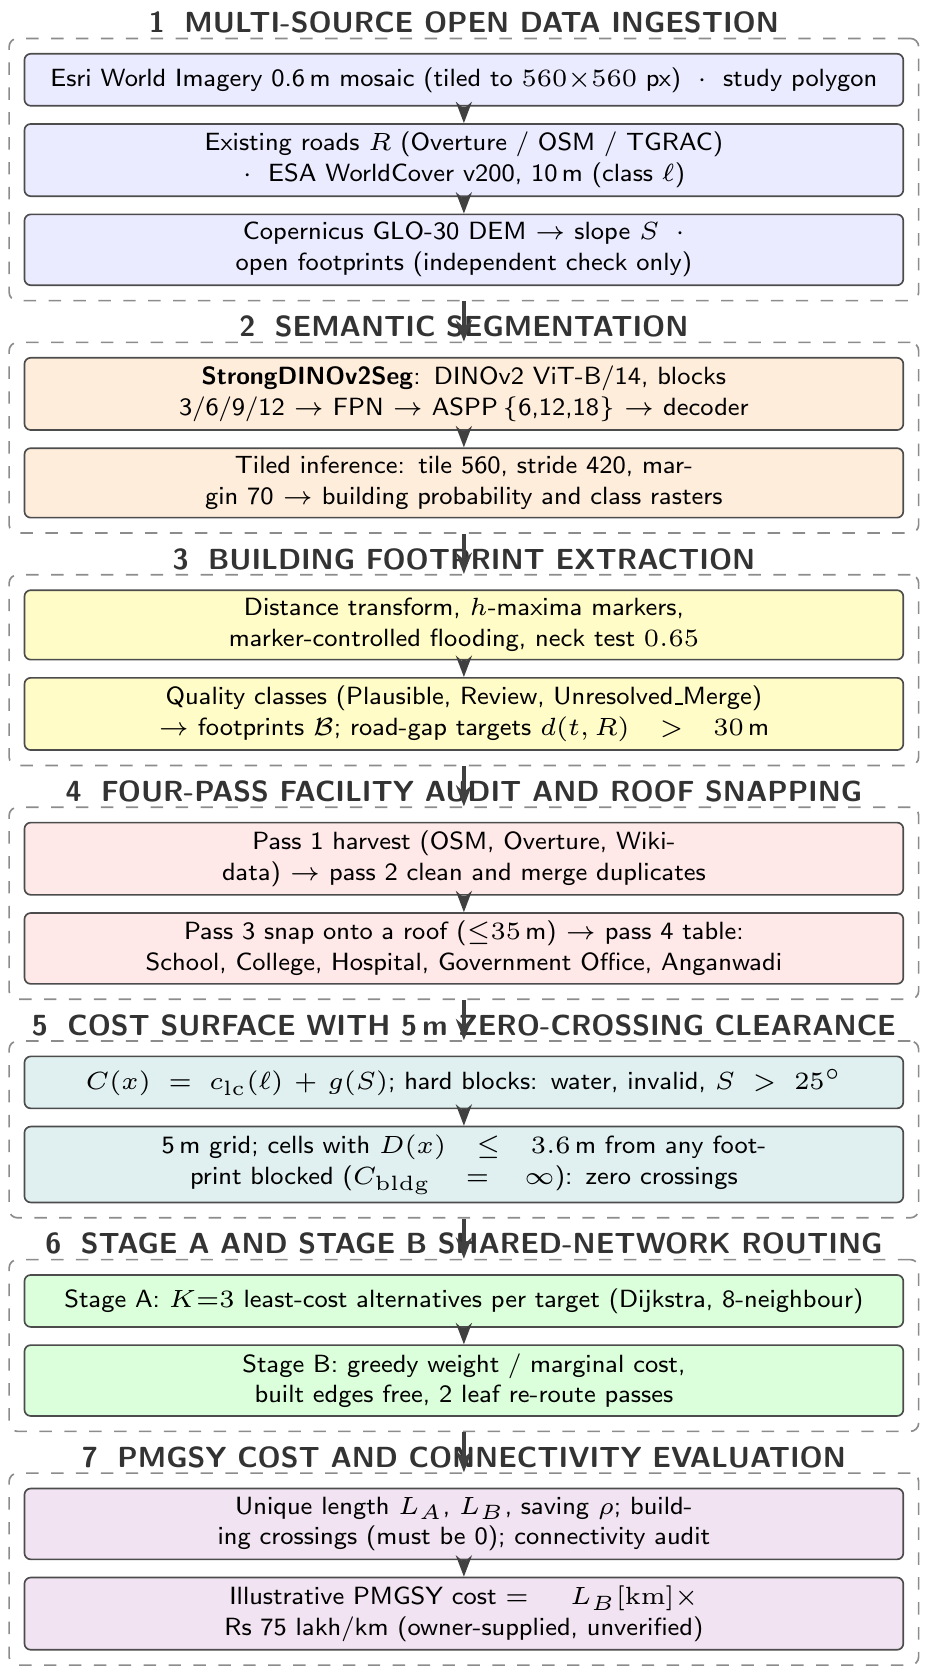
\includegraphics[width=0.5\textwidth]{figures/fig_architecture.png}
\caption{Seven-step architecture: (1)~multi-source open-data ingestion, (2)~\dinoseg{} semantic segmentation (tile 560, stride 420, margin 70), (3)~distance-transform building footprint extraction (neck ratio 0.65), (4)~four-pass multi-source facility audit and roof snapping (School, College, Hospital, Government Office, Anganwadi), (5)~cost surface with a 5~m zero-crossing clearance (3.6~m), (6)~Stage~A independent and Stage~B shared-network Dijkstra routing, (7)~PMGSY cost and connectivity evaluation.}
\label{fig:arch}
\end{figure}

\subsection{Building extraction}
\dinoseg{} is a fully fine-tuned DINOv2 ViT-B/14 encoder \cite{oquab2023dinov2}. Tokens from blocks 3, 6, 9 and 12 are projected to 256 channels, fused (FPN-style \cite{lin2017fpn}), passed through an ASPP neck (rates 6, 12, 18) \cite{chen2018deeplabv3plus} and a four-stage decoder with auxiliary heads for deep supervision \cite{lee2015dsn}. Training used LoveDA \cite{wang2021loveda} at 560~px for a scheduled 10 epochs (AdamW, cosine schedule to $10^{-7}$, encoder learning rate $\times 0.1$) with loss $0.5\,\mathrm{CE}+0.4\,\mathrm{Dice}+0.1\,\mathrm{edge}$ \cite{milletari2016vnet} and auxiliary weight 0.4. The epoch-4 checkpoint was used; the file used for the Adilabad run has SHA-256 \texttt{2e7c4646dc77ceb2\allowbreak a357f44f11cb3f7f\allowbreak f84e636871d70ba4\allowbreak c31e194e5ec00cf3}. Building instances are extracted from the predicted mask with OpenCV and NumPy: h-maxima of the distance transform give markers, a neck test (ratio 0.65) decides whether touching blobs are split, and blobs that cannot be split are flagged \textsc{Unresolved\_Merge}.

\subsection{Road-gap targets and Adilabad footprint sources}
For Adilabad the same imagery-to-footprint chain is run on Esri imagery (Section~\ref{sec:adilabad_data}), and Overture footprints serve as an independent check. Because connecting every footprint is meaningless in a built-up fabric already served by roads, only houses more than 30~m (the planner snap distance) from an existing road are routed. Planner cost grows roughly quadratically with the number of targets, which further motivates the filter; the threshold is varied (20, 30, 50~m) in Section~\ref{sec:adilabad}.

\subsection{Cost surface}
Let $\mathcal{B}$ be blocked cells (water, invalid cells, slope $>25^{\circ}$) and $\mathcal{P}$ the cells whose centre lies inside a footprint. The graph has the unblocked 10~m cells as nodes and 8-neighbour edges with no diagonal corner-cutting. The cell cost is
\begin{equation}
c(x)=\bigl[c_{\mathrm{lc}}(\ell(x))+g(s(x))\bigr]\,m(x),\qquad m(x)=\begin{cases}\mu & x\in\mathcal{P}\\ 1 & \text{otherwise,}\end{cases}
\label{eq:cell}
\end{equation}
where $\ell$ is the WorldCover class with resistance $c_{\mathrm{lc}}=8,5,3,6,2,4$ for trees, shrubland, grassland, cropland, built-up and bare/sparse land respectively (classes 10--60 in the order 10, 20, 30, 40, 50, 60), $g(s)=4\,\mathrm{clip}(s,0,10)/10$ with $s$ the slope in degrees, and $\mu=4$ is the footprint penalty. Edge weights are the mean end-cell cost times step length. Costs are ordinal planning units, not currency. In Damarakunta the penalty is lifted within a 20~m disc around the health sub-centre,  The land-cover, slope, cost and blocked-cell rasters are the inputs of the cost surface of every study area (figure~\ref{fig:flow}).whose point lies on the edge of its own footprint.

\subsection{Shared-network planner}
For each target, Stage~A computes a least-cost path to the existing road cells with Dijkstra's algorithm \cite{dijkstra1959note,hart1968astar,collischonn2000lcp} and alternatives by inflating costs along earlier paths ($K=3$ alternatives in total). Stage~B greedily selects the (target, alternative) pair with the highest weight per marginal cost
\begin{equation}
\Delta\Lcost\bigl(\pi\mid S\bigr)=\sum_{e\in\pi\setminus E_S}w(e),
\label{eq:marginal}
\end{equation}
where $E_S$ is the set of already selected edges, so built edges are free and a route may end on another route. This is the shortest-path heuristic for Steiner trees \cite{kou1981steiner,mehlhorn1988steiner} on a penalised, land-cover-weighted graph with the road network as a free sub-tree; it carries no optimality guarantee. Two passes of leaf re-routing follow. Snap distance is 30~m, search limit 1{,}500~m and attachment tolerance 15~m. Facilities are planned in a separate phase.

\subsection{Facility audit and roof snapping}
Overture Places alone mislocated or missed colleges, hospitals, offices and anganwadis, so the facilities of each area come from a four-pass audit (\texttt{scripts/audit\_facilities.py}). Pass~1 harvests candidates inside and within 500~m of the polygon from OpenStreetMap (Overpass and the Photon geocoder), Overture Places, Wikidata and Wikipedia (and, for Damarakunta, the TGRAC layers); LGD, UDISE+ and the district directories have no open query interface and were not used. Pass~2 assigns one of five categories (School, College, Hospital, Government Office, Anganwadi), removes closed or commercial records (pharmacies, laboratories, coaching centres, banks, cooperative societies), religious sites, foreign place names, placeholder coordinates shared by several differently named records, and merges duplicates of one campus across sources; every removal is logged with its reason. Pass~3 moves each survivor onto the footprint that contains it or, failing that, the nearest footprint of at least 25~m$^2$ within 35~m (a compound building up to 25~m away for a school, college or hospital), and removes facilities with no building in range. Pass~4 writes the verified table with the sources, the snap distance and a confidence label; records with a single source and a snap of more than 12~m are kept with \texttt{use\_in\_analysis}${}=$\,False and are not routed.

\subsection{Zero-crossing building clearance}
The soft footprint penalty $\mu$ in equation~\ref{eq:cell} lets a route cross a roof when the detour costs more. The proposed plan therefore uses a hard barrier on a finer grid. Each 10~m cost cell is refined to $2\times2$ cells of cell size $\Delta=5$~m with the same cost per metre, and every cell whose centre lies within $r_c=3.6$~m of any footprint is blocked (equation~\ref{eq:bldg}). Because $r_c>\Delta\sqrt2/2=3.54$~m, no step between two free cell centres can touch a footprint: a point of the step lies within $\Delta\sqrt2/2$ of one of its end points, and that end point would then have been blocked. A target sits inside its own building, so each route starts at the edge of that building and reaches the nearest free cell that is connected to the road network by a straight lane of at most the snap distance that touches no other footprint; a target with no such lane (a house enclosed by other buildings) is reported as unrouted, never routed over a roof. Lengths are measured from the building edge. Every drawn route (lane, path and attachment to a road) is finally intersected with all footprints other than its own.

\subsection{Mathematical formulation}
\paragraph{Segmentation loss.} With logits $\mathbf z$, labels $y$, class probabilities $p_{ic}$ and one-hot targets $t_{ic}$ at pixel $i$ (class 0 is ignored),
\begin{equation}
\mathcal L(\mathbf z,y)=0.5\,\mathcal L_{\mathrm{CE}}+0.4\,\mathcal L_{\mathrm{Dice}}+0.1\,\mathcal L_{\mathrm{edge}},\qquad
\mathcal L_{\mathrm{total}}=\mathcal L(\mathbf z^{\mathrm{main}},y)+0.4\sum_{j=1}^{3}\mathcal L(\mathbf z^{(j)},y),
\label{eq:loss}
\end{equation}
\begin{equation}
\mathcal L_{\mathrm{Dice}}=\frac1{|\mathcal C|}\sum_{c\in\mathcal C}\Bigl(1-\frac{2\sum_i p_{ic}t_{ic}+\varepsilon}{\sum_i p_{ic}+\sum_i t_{ic}+\varepsilon}\Bigr),\qquad
\mathcal L_{\mathrm{edge}}=\frac1{|\Omega|}\sum_{i\in\Omega}(1+4e_i)\,\mathrm{CE}_i,\quad e_i=\min\{1,\,|(K_x{*}y)_i|+|(K_y{*}y)_i|\}.
\label{eq:diceedge}
\end{equation}
Here $\mathcal C$ is the set of scored classes, $\varepsilon$ a small smoothing constant, $K_x,K_y$ the Sobel kernels, so that the edge term up-weights the cross-entropy of pixels on label boundaries by up to five; the three auxiliary heads $\mathbf z^{(j)}$ provide deep supervision.

\paragraph{Evaluation metrics.} From the confusion matrix, with $TP_c,FP_c,FN_c$ the true positives, false positives and false negatives of class $c$ and $N$ the number of labelled pixels,
\begin{equation}
\mathrm{OA}=\frac{\sum_c TP_c}{N},\quad P_c=\frac{TP_c}{TP_c+FP_c},\quad R_c=\frac{TP_c}{TP_c+FN_c},\quad F_{1,c}=\frac{2P_cR_c}{P_c+R_c}=\frac{2TP_c}{2TP_c+FP_c+FN_c},\quad \mathrm{IoU}_c=\frac{TP_c}{TP_c+FP_c+FN_c},
\label{eq:metrics}
\end{equation}
and $P$, $R$, $F_1$ (the Dice coefficient) and $\mathrm{mIoU}=|\mathcal C|^{-1}\sum_{c\in\mathcal C}\mathrm{IoU}_c$ are the macro averages over the scored classes. Because $F_{1,c}$ equals the per-class Dice score, the reported F1-score is the mean Dice.

\paragraph{Terrain.} Slope is taken from the Copernicus GLO-30 elevation $z$ with the Sobel gradient at the DEM spacing $\Delta_z=30$~m, resampled bilinearly to the planning grid:
\begin{equation}
\partial_x z\approx\frac{(K_x{*}z)}{8\Delta_z},\quad \partial_y z\approx-\frac{(K_y{*}z)}{8\Delta_z},\quad S=\arctan\sqrt{(\partial_x z)^2+(\partial_y z)^2},\quad p_S=100\tan S,
\label{eq:slope}
\end{equation}
with $S$ the slope in degrees and $p_S$ the equivalent percentage slope reported in the comparison table. The cost uses the linear ramp $g(S)=w_s\min(S,S_{\mathrm{ref}})/S_{\mathrm{ref}}$ with $w_s=4$ and $S_{\mathrm{ref}}=10^{\circ}$, and cells with $S>S_{\lim}=25^{\circ}$ are blocked; no separate IRC slope-penalty factor is applied.

\paragraph{Composite cost and clearance barrier.} With $c_{\mathrm{lc}}(\ell)$ the WorldCover resistance (equation~\ref{eq:cell}, so the land-cover weight is $w_{\mathrm{lc}}=1$) and $D(x)$ the Euclidean distance from the centre of cell $x$ to the nearest footprint (zero inside a footprint),
\begin{equation}
C(x)=c_{\mathrm{lc}}(\ell(x))+g(S(x))+C_{\mathrm{bldg}}(x),\qquad C_{\mathrm{bldg}}(x)=\begin{cases}\infty & D(x)\le r_c\\ 0 & \text{otherwise,}\end{cases}\qquad r_c=3.6\ \mathrm{m},\ \Delta=5\ \mathrm{m}.
\label{eq:bldg}
\end{equation}
The ten-metre comparison baseline instead multiplies the cost of cells whose centre lies in a footprint by $\mu=4$ (equation~\ref{eq:cell}).

\paragraph{Graph and routing objectives.} The graph has the free cells as nodes and 8-neighbour edges, a diagonal step being allowed only if both orthogonal neighbours are free. The weight of an edge $(u,v)$ is
\begin{equation}
w(u,v)=d(u,v)\,\frac{C(u)+C(v)}{2},\qquad d(u,v)=\begin{cases}\Delta&\text{cardinal step}\\ \sqrt2\,\Delta&\text{diagonal step.}\end{cases}
\label{eq:edge}
\end{equation}
Stage~A gives every target $t$ the independent least-cost path $\pi_t^{A}=\arg\min_{\pi:\,t\to R}\sum_{e\in\pi}w(e)$ to the existing road cells $R$ (Dijkstra), and two further alternatives that multiply $w(e)$ by $\lambda\in\{3,8\}$ on cells within $20$~m of the earlier paths and overlap them by at most 80\%. Stage~B starts from $E_S=\emptyset$ and repeatedly serves the target and route with the highest weight per marginal cost,
\begin{equation}
(t^\star,\pi^\star)=\arg\max_{t\in U,\ \pi\in\Pi_t\cup\{\pi_t^{\mathrm{net}}\}}\frac{\omega_t}{\Delta\Lcost(\pi\mid S)},\qquad
\Delta\Lcost(\pi\mid S)=\sum_{e\in\pi\setminus E_S}w(e),
\label{eq:stageb}
\end{equation}
where $U$ is the set of unserved targets, $\Pi_t$ the Stage~A alternatives, $\pi_t^{\mathrm{net}}$ the least-cost path to the roads together with the routes already selected, and $\omega_t$ the priority weight ($4$ for hospitals and health centres, $3$ for schools, colleges and anganwadis, $2$ for government offices, $1$ for houses). A built edge $e\in E_S$ thus costs nothing again, which is a discount factor $\alpha=0$ on $E_S$; no intermediate $\alpha\in(0,1)$ is used. With $L(\cdot)$ the total length of the unique edges of a route set (shared edges once),
\begin{equation}
\rho=\frac{L_A-L_B}{L_A}\times100\%,\qquad L_A=L\bigl(\{\pi_t^A\}\bigr),\quad L_B=L(E_S),\qquad X=\sum_{r}\Bigl|r\cap\bigcup_{b\ne b_r}b\Bigr|=0,
\label{eq:saving}
\end{equation}
where $X$ is the length of routes inside footprints other than the route's own building $b_r$ (zero by construction under equation~\ref{eq:bldg}).

\paragraph{Illustrative cost.} The capital cost is
\begin{equation}
\mathrm{Cost}_{\mathrm{INR\ lakh}}=L_B[\mathrm{km}]\times c_{\mathrm{PMGSY}},\qquad c_{\mathrm{PMGSY}}=75\ \text{lakh/km}\ (\text{range }60\text{--}90),
\label{eq:cost}
\end{equation}
with 1 lakh $=10^{5}$~INR. The rate was supplied by the project owner as PMGSY-based and has not been verified against a PMGSY document or a State Schedule of Rates, so the cost is illustrative and not an engineering estimate.

\subsection{Algorithms}
\begin{algorithm}[t]
\caption{Tiled \dinoseg{} inference and distance-transform building extraction (\texttt{run\_tiled\_inference.py}, \texttt{extract\_buildings\_v8.py})}
\label{alg:extract}
\begin{algorithmic}[1]
\Require mosaic $I$ (0.6~m), checkpoint $\theta$, tile $T=560$, stride $s=420$, margin $m=70$, neck ratio $\eta=0.65$, seed height $h=0.3$~m
\Ensure footprints $\mathcal B$ with quality classes
\State \textbf{assert} $s\le T-2m$ \Comment{no gaps between tile centres}
\For{each tile of size $T\times T$ at stride $s$}
  \State $p\gets\mathrm{softmax}(f_\theta(\text{tile}))$; write class $\arg\max p$ and $p_{\mathrm{bldg}}$ for the tile centre (drop $m$ px at inner edges)
\EndFor
\State $M\gets(\text{class}=\text{building})\wedge\lnot\text{no-data}$; drop components smaller than 6~m$^2$
\For{each connected component $K$ of $M$}
  \State $D\gets\mathrm{EDT}(K)$ (smoothed, $\sigma=1$ px); markers $\gets$ $h$-maxima of $D$ with height $h$
  \State pieces $\gets$ marker-controlled flooding of $-D$ (only if area $\ge 40$~m$^2$)
  \For{each adjacent piece pair $(a,b)$}
    \State $r_{ab}\gets D_{\mathrm{saddle}}/\min(D_a^{\max},D_b^{\max})$
    \If{$r_{ab}>\eta$ \textbf{or} a piece is smaller than 12~m$^2$} merge $a,b$ \Comment{no real neck}
    \EndIf
  \EndFor
\EndFor
\State polygonise; flag \textsc{Unresolved\_Merge} if area $>4\times$ the median compact roof; assign \textsc{Plausible} / \textsc{Review} / \textsc{Small} by confidence and shape
\State \Return $\mathcal B$
\end{algorithmic}
\end{algorithm}

\begin{algorithm}[t]
\caption{Cost surface with zero-crossing clearance and two-stage routing (\texttt{clearance.py}, \texttt{plan\_network\_v2.py})}
\label{alg:route}
\begin{algorithmic}[1]
\Require land cover $\ell$, DEM $z$, roads $R$, footprints $\mathcal B$, targets $\mathcal T$ (road-gap houses and verified facilities with weights $\omega_t$), $\Delta=5$~m, $r_c=3.6$~m, $K=3$
\Ensure route sets $\{\pi_t^A\}$, $E_S$ and lengths $L_A$, $L_B$, saving $\rho$, cost
\State $S\gets$ slope of $z$ (equation~\ref{eq:slope}); $C_0(x)\gets c_{\mathrm{lc}}(\ell(x))+g(S(x))$; block water, invalid cells and $S>25^{\circ}$
\State refine $C_0$ from 10~m to $\Delta=5$~m (same cost per metre); $D\gets\mathrm{EDT}(\mathcal B)$; $C(x)\gets\infty$ where $D(x)\le r_c$
\State keep the free cells connected to a road cell; edge weights $w$ by equation~\ref{eq:edge}
\For{each target $t\in\mathcal T$}
  \State entrance $e_t\gets$ point of the target's building edge nearest to a free cell $s_t$; require a lane $e_t\to s_t$ of at most 30~m that touches no other footprint, else mark $t$ unrouted
  \State $\Pi_t\gets K$ Dijkstra alternatives from $s_t$ to $R$ (corridor inflation $\lambda\in\{3,8\}$, 20~m, overlap $\le 80\%$); $\pi_t^A\gets$ first alternative
\EndFor
\State $L_A\gets L(\{\pi_t^A\})$; $U\gets$ routed targets; $E_S\gets\emptyset$
\While{$U\ne\emptyset$}
  \For{each $t\in U$} add the least-cost path $\pi_t^{\mathrm{net}}$ to $R\cup E_S$ to the candidates $\Pi_t$ \EndFor
  \State $(t^\star,\pi^\star)\gets\arg\max\ \omega_t/\Delta\Lcost(\pi\mid S)$ (equation~\ref{eq:stageb}); $E_S\gets E_S\cup\pi^\star$; $U\gets U\setminus\{t^\star\}$
\EndWhile
\State two leaf re-route passes: replace a route that no other route uses if it has become cheaper given the others
\State verify $X=0$ (equation~\ref{eq:saving}); $L_B\gets L(E_S)$; $\rho\gets 100(L_A-L_B)/L_A$; cost by equation~\ref{eq:cost}
\end{algorithmic}
\end{algorithm}

\subsection{Baselines, scenarios and metrics}
Four baselines are compared: straight lines, independent least-cost routes, a length-only control (cost surface replaced by distance) and a roads-only shared reference (routes may share edges only with the existing road network). The saving against independent routing is $\rho=(L_{\mathrm{ind}}-L)/L_{\mathrm{ind}}$, with $L$ the unique network length (shared edges counted once). The exposure metrics are the number of routes crossing another house's footprint and the route length inside other footprints. The footprint penalty is varied ($\mu\in\{1,4,20,100\}$, with a variant in which footprints are buffered by 7.1~m). For omissions, a target set $M$ is removed from the targets and from the penalty layer (a missed detection is absent from both), and the planner is re-run; random draws use seeds 1--5. Coverage, unserved households, change in unique length and length per routed target are reported.

\section{Results: Damarakunta}\label{sec:damar}
\subsection{Detection}
On the 1{,}669-image LoveDA validation split (560~px, seven scored classes) the epoch-4 checkpoint reached 53.8\% mIoU, 68.9\% Dice and 71.3\% pixel accuracy, with 72.4\% macro precision and 66.9\% macro recall; for the Building class IoU is 54.0\%, precision 62.1\% and recall 80.6\% (table~\ref{tab:seg}). These are source-domain figures, not accuracy on Damarakunta. Against Google Open Buildings v3 as a proxy (not ground truth), 118 of the 165 in-boundary candidates agree (71.5\%).

\begin{table}[t]
\caption{Detection evaluation. Top: LoveDA validation (source domain); precision and recall are macro-averages over the seven scored classes. Bottom: agreement of the 165 Damarakunta candidates with Open Buildings v3 (a proxy, not accuracy).}
\label{tab:seg}
\centering
\small
\begin{tabular}{@{}lrrrrr@{}}
\toprule
\multicolumn{6}{@{}l}{\textit{LoveDA validation split (\%)}}\\
 & mIoU & Dice & Pixel acc. & Precision & Recall\\
\midrule
StrongDINOv2Seg & 53.8 & 68.9 & 71.3 & 72.4 & 66.9\\
\quad Building class & 54.0 & 70.1 & --- & 62.1 & 80.6\\
\midrule
\multicolumn{6}{@{}l}{\textit{Damarakunta candidates vs.\ Open Buildings v3}}\\
Class & Candidates & Agree & Disagree & \multicolumn{2}{c}{Agreement (\%)}\\
\midrule
All & 165 & 118 & 47 & \multicolumn{2}{c}{71.5}\\
\textsc{Plausible} & 71 & 51 & 20 & \multicolumn{2}{c}{71.8}\\
\textsc{Review} & 32 & 14 & 18 & \multicolumn{2}{c}{43.8}\\
\textsc{Unresolved\_Merge} & 62 & 53 & 9 & \multicolumn{2}{c}{85.5}\\
\bottomrule
\end{tabular}
\end{table}

\subsection{Shared network and footprint penalty}
Independent least-cost routes for the 163 houses total 10{,}045~m, but because neighbouring houses re-trace the same corridors the unique built length is 6{,}753~m (table~\ref{tab:routing}, figure~\ref{fig:routing}a). The two-stage plan reduces this to 5{,}069~m, a saving of 24.9\%; all 163 houses and five facilities are connected. The length-only control is 3.4\% \emph{longer} in unique length than independent cost-surface routing, and the roads-only shared reference saves 22.6\%, so most of the saving comes from sharing and a further 2.3 percentage points from sharing between new routes.

The penalty trades length for exposure (figure~\ref{fig:routing}b). With $\mu=1$ the plan is shortest (4{,}705~m) but 56 routes pass through other houses (660~m inside footprints). With $\mu=4$ it is 7.7\% longer while crossings halve to 28 routes and 209~m. Buffering footprints by 7.1~m with $\mu=20$ or 100 lowers crossings further (19 routes) at 6{,}190--6{,}238~m.

\begin{table}[t]
\caption{Damarakunta routing, 163 houses ($\mu=4$ unless stated). Total length counts every route; unique length counts shared edges once; $\rho$ is the saving in unique length against independent routes.}
\label{tab:routing}
\centering
\footnotesize
\begin{tabular}{@{}>{\raggedright\arraybackslash}p{4.3cm}rrrrr@{}}
\toprule
Strategy & Total (m) & Unique (m) & $\rho$ (\%) & Routes crossing & In footprints (m)\\
\midrule
Straight line (2 targets infeasible) & 8{,}092.3 & --- & --- & 60 & 1{,}453.2\\
Independent least-cost routes & 10{,}045.4 & 6{,}753.1 & 0.0 & 46 & 328.3\\
Length-only control & 9{,}166.3 & 6{,}979.8 & $-3.4$ & 64 & 1{,}615.8\\
Roads-only shared reference & 5{,}229.3 & 5{,}229.3 & 22.6 & 29 & 216.1\\
\textbf{Two-stage plan (proposed)} & \textbf{5{,}069.0} & \textbf{5{,}069.0} & \textbf{24.9} & \textbf{28} & \textbf{209.1}\\
\midrule
\multicolumn{6}{@{}l}{\textit{No footprint penalty ($\mu=1$)}}\\
Independent least-cost routes & 9{,}595.9 & 6{,}921.3 & 0.0 & 63 & 1{,}423.1\\
Two-stage plan & 4{,}705.5 & 4{,}705.4 & 32.0 & 56 & 660.1\\
\midrule
\multicolumn{6}{@{}l}{\textit{Buffered footprints (7.1~m), two-stage plan}}\\
Penalty $\mu=20$ & --- & 6{,}238.1 & 18.5 & 19 & 147.9\\
Penalty $\mu=100$ & --- & 6{,}190.3 & 18.9 & 19 & 144.8\\
\bottomrule
\end{tabular}
\end{table}

\begin{figure}[t]
\centering
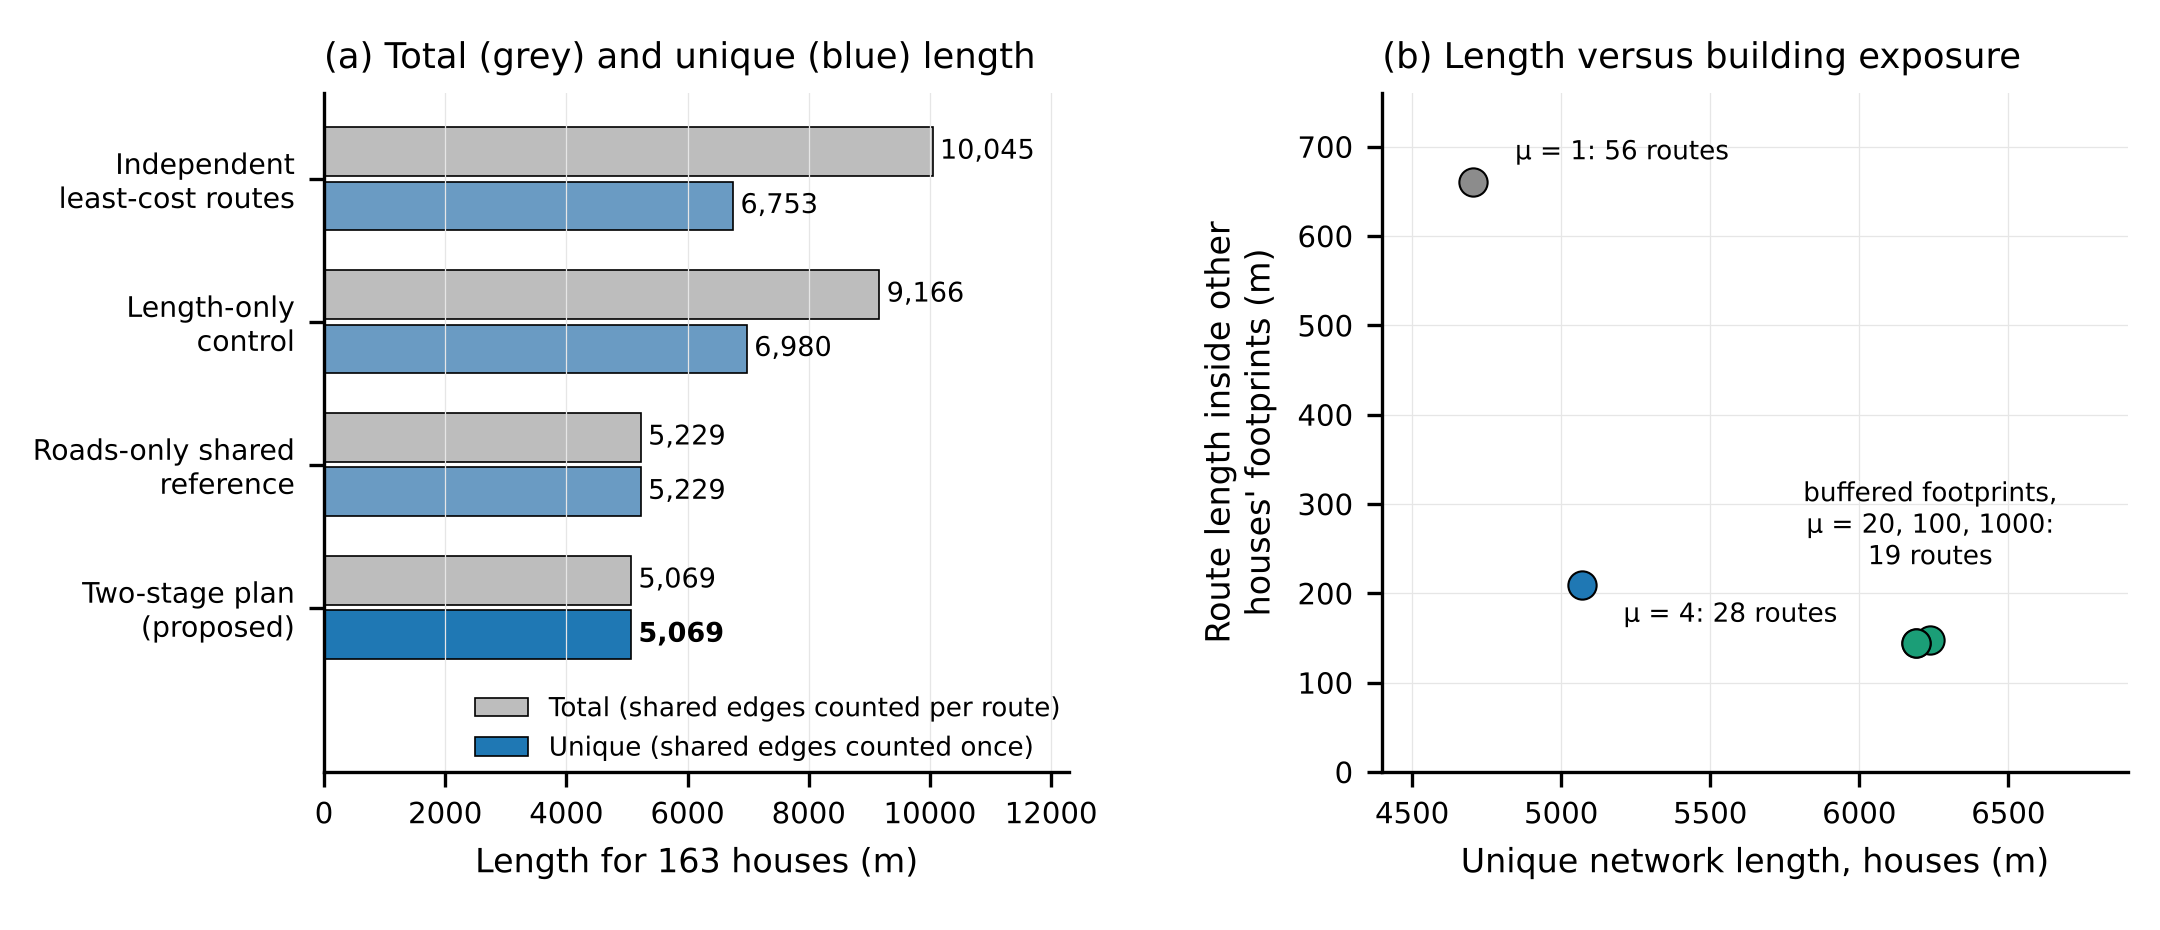
\includegraphics[width=\textwidth]{figures/fig3_routing.png}
\caption{Damarakunta routing results for 163 houses. (a)~Total and unique corridor length by strategy. (b)~Unique network length against route length inside other houses' footprints for $\mu=1$, $\mu=4$ and buffered footprints with large penalties.}
\label{fig:routing}
\end{figure}

\subsection{Impact of building omissions}
Table~\ref{tab:omission} and figure~\ref{fig:omission} summarise the omission analysis against the 5{,}069~m baseline. Missing buildings make the plan \emph{shorter}: 10\% random omission (16 houses) understates length by 7.6\%, 20\% by 16.9\%, omission of the smallest quarter by 25.1\% and omission of all merged blobs by 29.4\%. At the same time $U$ households lose access: 16 and 33 for random 10\% and 20\% omission, 41 for the smallest quarter and 62 (38.0\%) for merged blobs. A planner reading only total length would therefore underfund the scheme. Random additions lengthen the plan by 8.6\% and 15.8\%. The saving $\rho$ stays within 24.9--26.6\% across omissions, so the benefit of sharing is robust to inventory error.

\begin{table}[t]
\caption{Impact of simulated omissions and additions, Damarakunta. Baseline 5{,}069.0~m, 163 routed. Random scenarios are means of five draws. $U$: households without a route; $\kappa$: coverage; $\delta_L$: change in unique length; $\bar\ell$: length per routed target; $\rho$: saving against independent routing.}
\label{tab:omission}
\centering
\small
\begin{tabular}{@{}lrrrrrrr@{}}
\toprule
Scenario & Routed & $U$ & $\kappa$ (\%) & $L$ (m) & $\delta_L$ (\%) & $\bar\ell$ (m) & $\rho$ (\%)\\
\midrule
Baseline & 163 & 0 & 100.0 & 5{,}069.0 & 0.0 & 31.1 & 24.9\\
Omit 10\% (random) & 147.0 & 16 & 90.2 & 4{,}684.4 & $-7.6$ & 31.9 & 25.1\\
Omit 20\% (random) & 130.0 & 33 & 79.8 & 4{,}211.5 & $-16.9$ & 32.4 & 24.9\\
Omit smallest 10\% & 146 & 17 & 89.6 & 4{,}648.6 & $-8.3$ & 31.8 & 24.9\\
Omit smallest 25\% & 122 & 41 & 74.8 & 3{,}798.3 & $-25.1$ & 31.1 & 25.6\\
Omit merged blobs & 101 & 62 & 62.0 & 3{,}579.0 & $-29.4$ & 35.4 & 26.6\\
\midrule
Add 10\% (random) & 177.4 & --- & --- & 5{,}502.4 & $+8.6$ & 31.0 & 25.6\\
Add 20\% (random) & 190.6 & --- & --- & 5{,}868.3 & $+15.8$ & 30.8 & 25.4\\
\bottomrule
\end{tabular}
\end{table}

\begin{figure}[t]
\centering
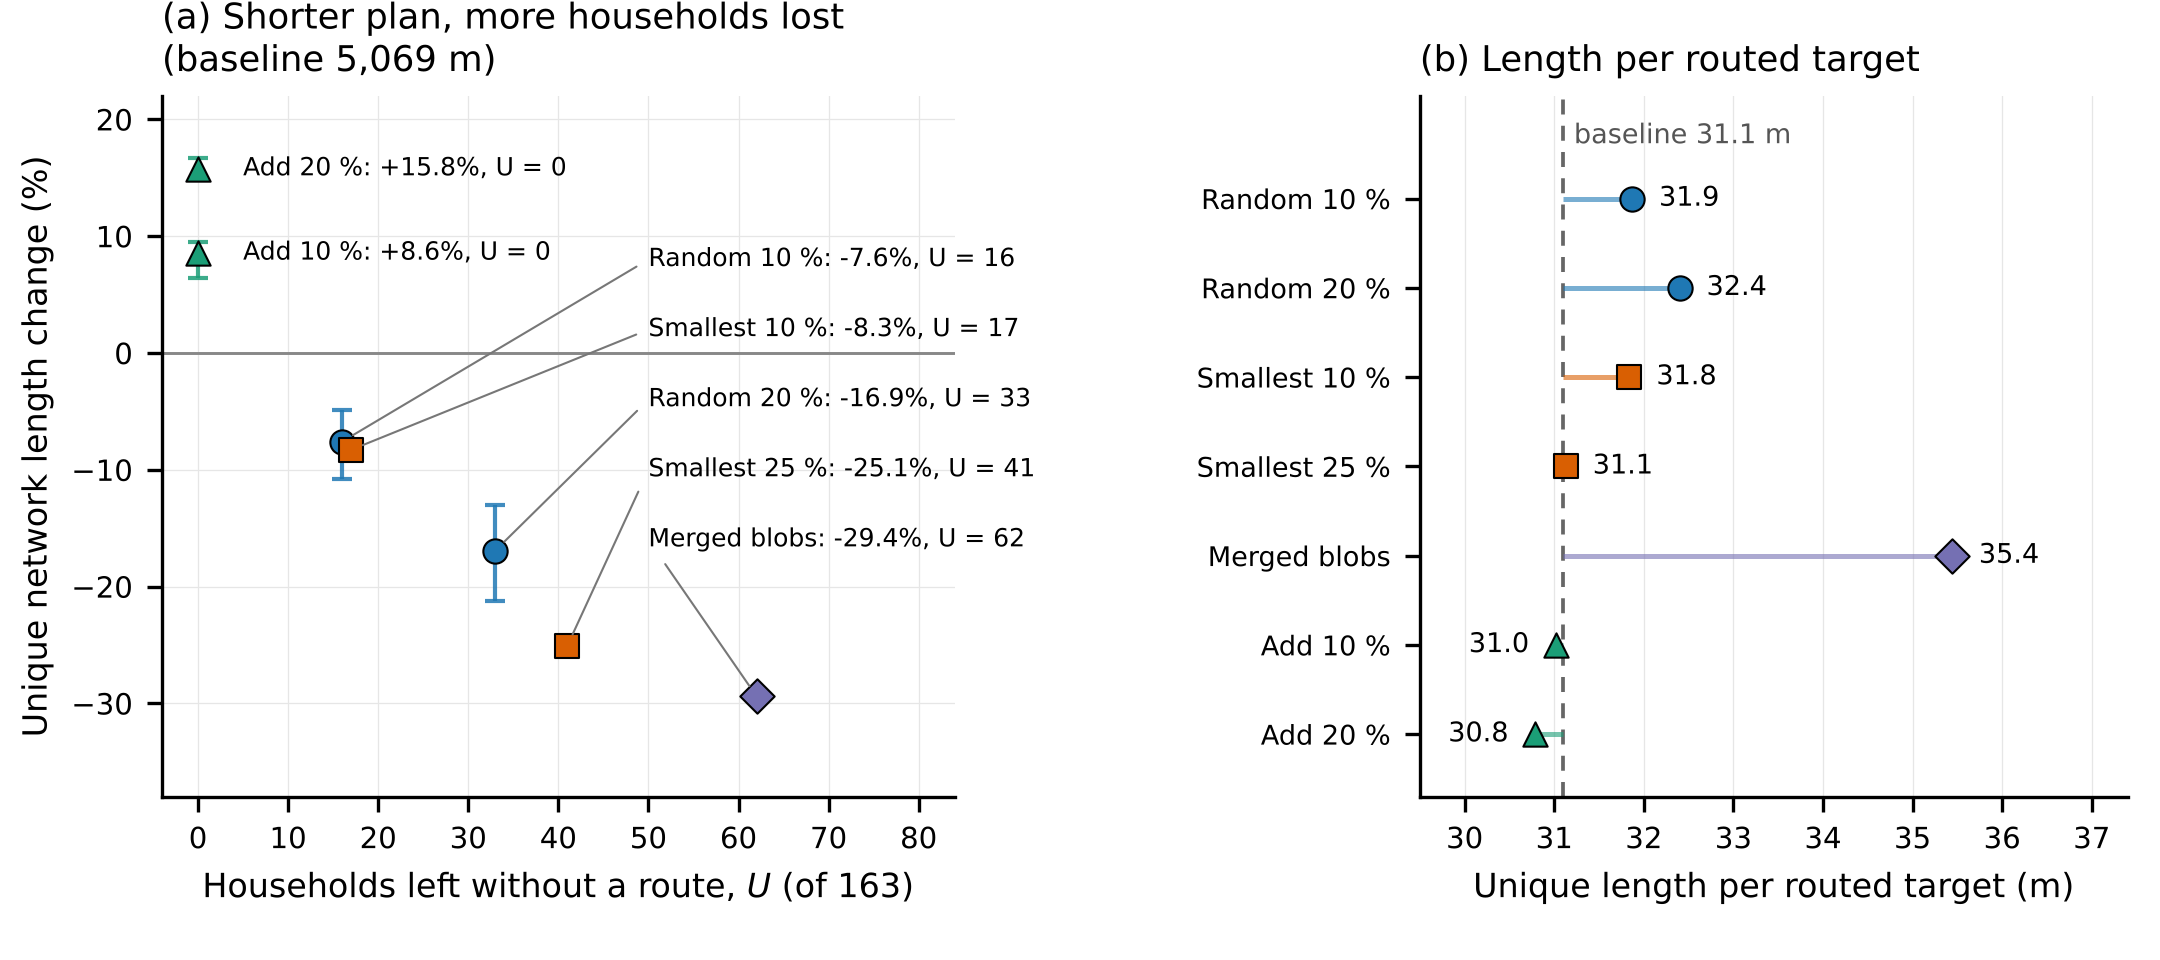
\includegraphics[width=\textwidth]{figures/fig4_omission.png}
\caption{Damarakunta omission sensitivity (163 baseline targets, 5{,}069~m; random scenarios are five draws with min--max bars). (a)~Change in unique length against households left without a route. (b)~Unique length per routed target.}
\label{fig:omission}
\end{figure}

\section{Results: transfer to Adilabad Urban}\label{sec:adilabad}
\subsection{Road-gap targets and routing}
\emph{End-to-end run (\dinoseg{} footprints).} Of the 2{,}690 footprints of at least 30~m$^2$, 345 lie more than 30~m from a road and form the targets (Damarakunta: 163). The planner routes all 345. Independent least-cost routes total 23{,}312.5~m (unique 21{,}440.8~m); the two-stage plan needs 18{,}288.7~m, a saving of 14.7\% (table~\ref{tab:adilabad}; the routes are drawn in figure~\ref{fig:flow}). The roads-only shared reference saves 2.3\% and the length-only control 6.9\%, so almost all of the saving comes from sharing among new routes. Exposure: 54 of 345 routes (15.7\%) cross another footprint (398.0~m), against 28 of 163 (17\%) in Damarakunta.

These numbers must be read with the extraction quality in mind. More than half of the instances (1{,}580 of 2{,}769) are \textsc{Unresolved\_Merge} blobs with a median area of 1{,}125.5~m$^2$: in the dense fabric the segmenter merges neighbouring roofs, so the 345 targets are built-up units rather than houses, and the footprint penalty acts on merged blocks. No reference mask exists for Adilabad, so detection accuracy there is not known.

\emph{Open-footprint check.} With 874 road-gap targets (873 routed) among 18{,}242 Overture footprints (median footprint 139.6~m$^2$, median distance to the nearest road 42.3~m), independent routes total 56{,}308.0~m (unique 46{,}419.2~m) and the two-stage plan 34{,}358.8~m, a saving of 26.0\%; the roads-only reference saves 2.9\% and the length-only control 5.7\%; 332 of 873 routes (38\%) cross another footprint (2{,}041.1~m). The facility phase connects 71 verified facilities with 1{,}090.1~m of unique corridor.

Both Adilabad variants agree that sharing helps (14.7\% and 26.0\%) and that a roads-only reference does not (2.3\% and 2.9\%, against 22.6\% in Damarakunta), but they differ in the size of the saving. This is consistent with fewer, more widely spaced targets (345 against 874) offering less opportunity to share, an explanation that was not tested. The comparison is between two footprint sources, not a validation of either.

\begin{table}[t]
\caption{Cross-settlement comparison under the same cost surface and solver. ``Seg.'' = \dinoseg{} footprints on Esri imagery; ``open'' = Overture footprints. Targets are defined by different rules (all candidates in Damarakunta, road-gap houses in Adilabad).}
\label{tab:adilabad}
\centering
\footnotesize
\begin{tabular}{@{}>{\raggedright\arraybackslash}p{5.6cm}rrr@{}}
\toprule
Metric & Damarakunta & Adilabad seg. & Adilabad open\\
\midrule
Study area (km$^2$) & 18.47 & 17.75 & 17.75\\
Targets / routed & 163 / 163 & 345 / 345 & 874 / 873\\
Independent routes, unique (m) & 6{,}753.1 & 21{,}440.8 & 46{,}419.2\\
Length-only control, unique (m) & 6{,}979.8 & 19{,}961.2 & 43{,}787.2\\
Roads-only shared reference, unique (m) & 5{,}229.3 & 20{,}947.0 & 45{,}058.9\\
\textbf{Two-stage plan, unique (m)} & \textbf{5{,}069.0} & \textbf{18{,}288.7} & \textbf{34{,}358.8}\\
Saving vs.\ independent (\%) & 24.9 & 14.7 & 26.0\\
Roads-only shared saving (\%) & 22.6 & 2.3 & 2.9\\
Unique length per routed house (m) & 31.1 & 53.0 & 39.4\\
Routes crossing other footprints & 28 of 163 & 54 of 345 & 332 of 873\\
Length inside other footprints (m) & 209.1 & 398.0 & 2{,}041.1\\
$\mu=1\rightarrow4$: unique length change (\%) & $+7.7$ & $+9.2$ & $+13.3$\\
$\mu=1\rightarrow4$: routes crossing & 56 $\rightarrow$ 28 & 138 $\rightarrow$ 54 & 618 $\rightarrow$ 332\\
10\% random omission: change (\%) / unserved & $-7.6$ / 16 & $-8.8$ / 34 & $-7.6$ / 88\\
20\% random omission: change (\%) / unserved & $-16.9$ / 33 & $-18.3$ / 69 & $-15.0$ / 176\\
Smallest-25\% omission: change (\%) / unserved & $-25.1$ / 41 & $-21.2$ / 87 & $-21.2$ / 220\\
\bottomrule
\end{tabular}
\end{table}
\subsection{Robustness}
\emph{Footprint penalty.} Raising $\mu$ from 1 to 4 lengthens the unique network by 9.2\% and removes 84 crossing routes (138 to 54); $\mu=20$ and 100 give 19{,}777.0~m and 19{,}924.5~m with 49 and 48 routes crossing, and buffered footprints give 22{,}757.0~m and 23{,}475.5~m with 7 crossing each (table~\ref{tab:sens}, figure~\ref{fig:adilsens}a). The saving against independent routing stays between 10.1\% and 17.7\% across all settings (open footprints: 17.8\% to 30.8\%, table~\ref{tab:sens_open}).

\emph{Road-gap threshold.} Targets defined as houses more than 20, 30 or 50~m from a road number 750, 345 and 129 and give savings of 10.6\%, 14.7\% and 18.5\% (open footprints: 2{,}190, 874 and 296 targets; 21.9\%, 26.0\% and 29.5\%). The saving therefore depends on the target definition, which should be reported with any such result.

\emph{Omissions.} Random omission of 10\% and 20\% (five seeds) changes unique length by $-8.8\%$ (range $-11.7$ to $-6.5$) and $-18.3\%$ ($-21.9$ to $-15.8$), leaving 34 and 69 targets unserved; single-run smallest-10\% and smallest-25\% omissions give $-8.0\%$ and $-21.2\%$ (35 and 87 unserved). As in Damarakunta and in the open-footprint check, missing buildings shorten the plan while stranding households, and the saving stays at 12.6--14.1\%. With open footprints the same scenarios give $-7.6\%$, $-15.0\%$, $-7.9\%$ and $-21.2\%$ and a saving of 23.8--25.2\%. Merged-blob and addition scenarios were not defined for Adilabad.

\begin{table}[t]
\caption{Adilabad sensitivity, \dinoseg{} footprints (345 targets unless stated). Top: footprint-penalty settings. Bottom: road-gap threshold.}
\label{tab:sens}
\centering
\footnotesize
\begin{tabular}{@{}lrrrrr@{}}
\toprule
Setting & Unique (m) & $\rho$ (\%) & Crossing routes & In footprints (m) & Targets\\
\midrule
Centre-in-footprint, $\mu=1$ & 16{,}740.5 & 17.7 & 138 & 1{,}479.8 & 345\\
Centre-in-footprint, $\mu=4$ & 18{,}288.7 & 14.7 & 54 & 398.0 & 345\\
Centre-in-footprint, $\mu=20$ & 19{,}777.0 & 12.5 & 49 & 356.4 & 345\\
Centre-in-footprint, $\mu=100$ & 19{,}924.5 & 12.2 & 48 & 343.2 & 345\\
Buffered 7.1~m, $\mu=20$ & 22{,}757.0 & 10.1 & 7 & 57.9 & 345\\
Buffered 7.1~m, $\mu=100$ & 23{,}475.5 & 10.6 & 7 & 55.7 & 345\\
\midrule
Gap $>20$~m & 30{,}621.7 & 10.6 & 69 & 442.8 & 750\\
Gap $>30$~m (primary) & 18{,}288.7 & 14.7 & 54 & 398.0 & 345\\
Gap $>50$~m & 9{,}155.2 & 18.5 & 28 & 251.9 & 129\\
\bottomrule
\end{tabular}
\end{table}

\begin{table}[t]
\caption{Adilabad sensitivity, open Overture footprints (874 targets, 873 routed). Top: footprint-penalty settings. Bottom: road-gap threshold.}
\label{tab:sens_open}
\centering
\footnotesize
\begin{tabular}{@{}lrrrrr@{}}
\toprule
Setting & Unique (m) & $\rho$ (\%) & Crossing routes & In footprints (m) & Targets\\
\midrule
Centre-in-footprint, $\mu=1$ & 30{,}335.7 & 30.8 & 618 & 4{,}893.0 & 874\\
Centre-in-footprint, $\mu=4$ & 34{,}358.8 & 26.0 & 332 & 2{,}041.1 & 874\\
Centre-in-footprint, $\mu=20$ & 37{,}024.1 & 22.8 & 271 & 1{,}687.4 & 874\\
Centre-in-footprint, $\mu=100$ & 37{,}513.9 & 21.7 & 275 & 1{,}744.8 & 874\\
Buffered 7.1~m, $\mu=20$ & 42{,}071.9 & 20.1 & 231 & 1{,}397.2 & 874\\
Buffered 7.1~m, $\mu=100$ & 44{,}094.6 & 17.8 & 221 & 1{,}310.5 & 874\\
\midrule
Gap $>20$~m & 65{,}204.4 & 21.9 & 815 & 4{,}543.9 & 2{,}190\\
Gap $>30$~m (primary) & 34{,}358.8 & 26.0 & 332 & 2{,}041.1 & 874\\
Gap $>50$~m & 15{,}880.9 & 29.5 & 126 & 809.9 & 296\\
\bottomrule
\end{tabular}
\end{table}

\begin{figure}[t]
\centering
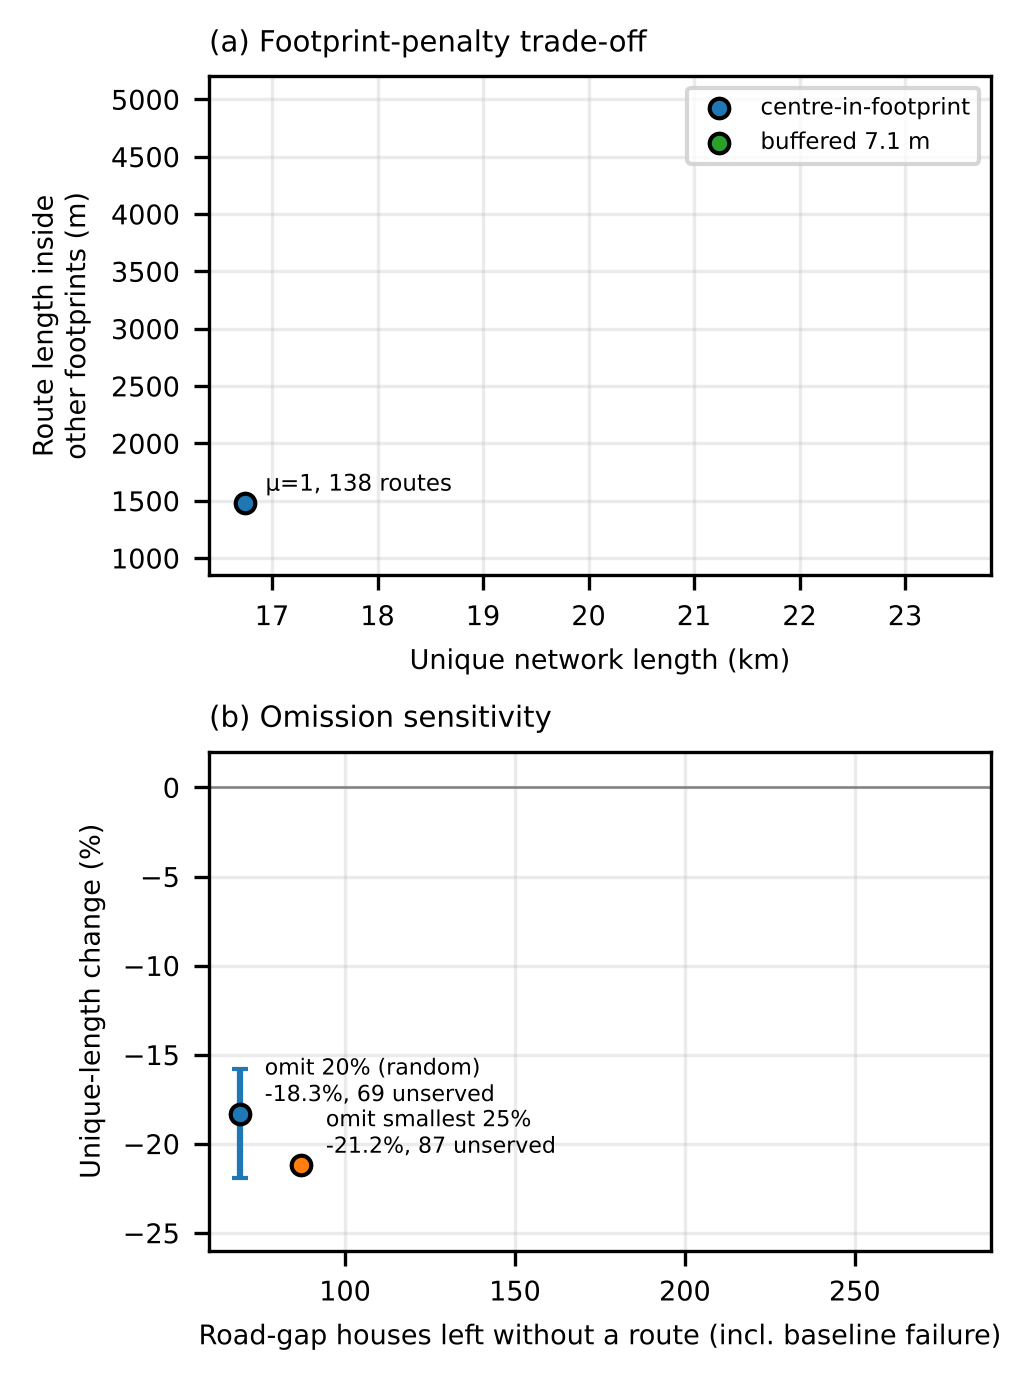
\includegraphics[width=0.5\textwidth]{figures/adilabad_seg_sens_col.png}
\caption{Adilabad sensitivity (\dinoseg{} footprints). (a)~Footprint-penalty trade-off between unique network length and route length inside other footprints. (b)~Omission sensitivity (random: mean and min--max over five seeds; smallest-$q$: single run).}
\label{fig:adilsens}
\end{figure}

\section{Results: four study areas with zero-crossing clearance}\label{sec:four}
Figure~\ref{fig:flow} follows the chain of figure~\ref{fig:arch} for the four study areas, from the Telangana locator through the input imagery and roads, the extracted footprints and verified facilities, to the planned network. Table~\ref{tab:four} collects every metric of the four areas in one place; it is regenerated by \texttt{scripts/run\_village\_pipeline.py --compare-all}, and a red \pending{value} marks a number not yet computed on the machine that wrote the table. The Adilabad column uses the updated settlement boundary (a derived built-up extent of Adilabad town) and the segmentation footprints of that boundary, so it is not the 2018 mandal experiment of the preceding sections.

On the 5~m clearance grid, Stage~B shortens the unique network relative to the independent Stage~A routes by Damarakunta 21.0\%, Adilabad 12.2\%, Aswaraopeta 25.3\%, Alampur 16.2\%. Building crossings are zero in every area by construction and were verified by intersecting every drawn route with all footprints, whereas the ten-metre soft-penalty plan ($\mu=4$) still leaves routes across other footprints (Damarakunta 28, Adilabad 99, Aswaraopeta 157, Alampur 5 routes, respectively). Targets with no free lane to the road network are reported as unrouted rather than routed over a roof, so the routed counts in table~\ref{tab:four} are below the target counts where buildings enclose a house. The segmentation rows are model-level: they are the LoveDA validation scores of the one checkpoint used for all four areas, not accuracy on any of the four areas, for which no surveyed reference exists. Costs use the owner-supplied, unverified PMGSY-based rate of Rs 75 lakh/km and are illustrative.

\begin{figure*}[p]
\centering
\IfFileExists{figures/fig_flow_study_areas.png}{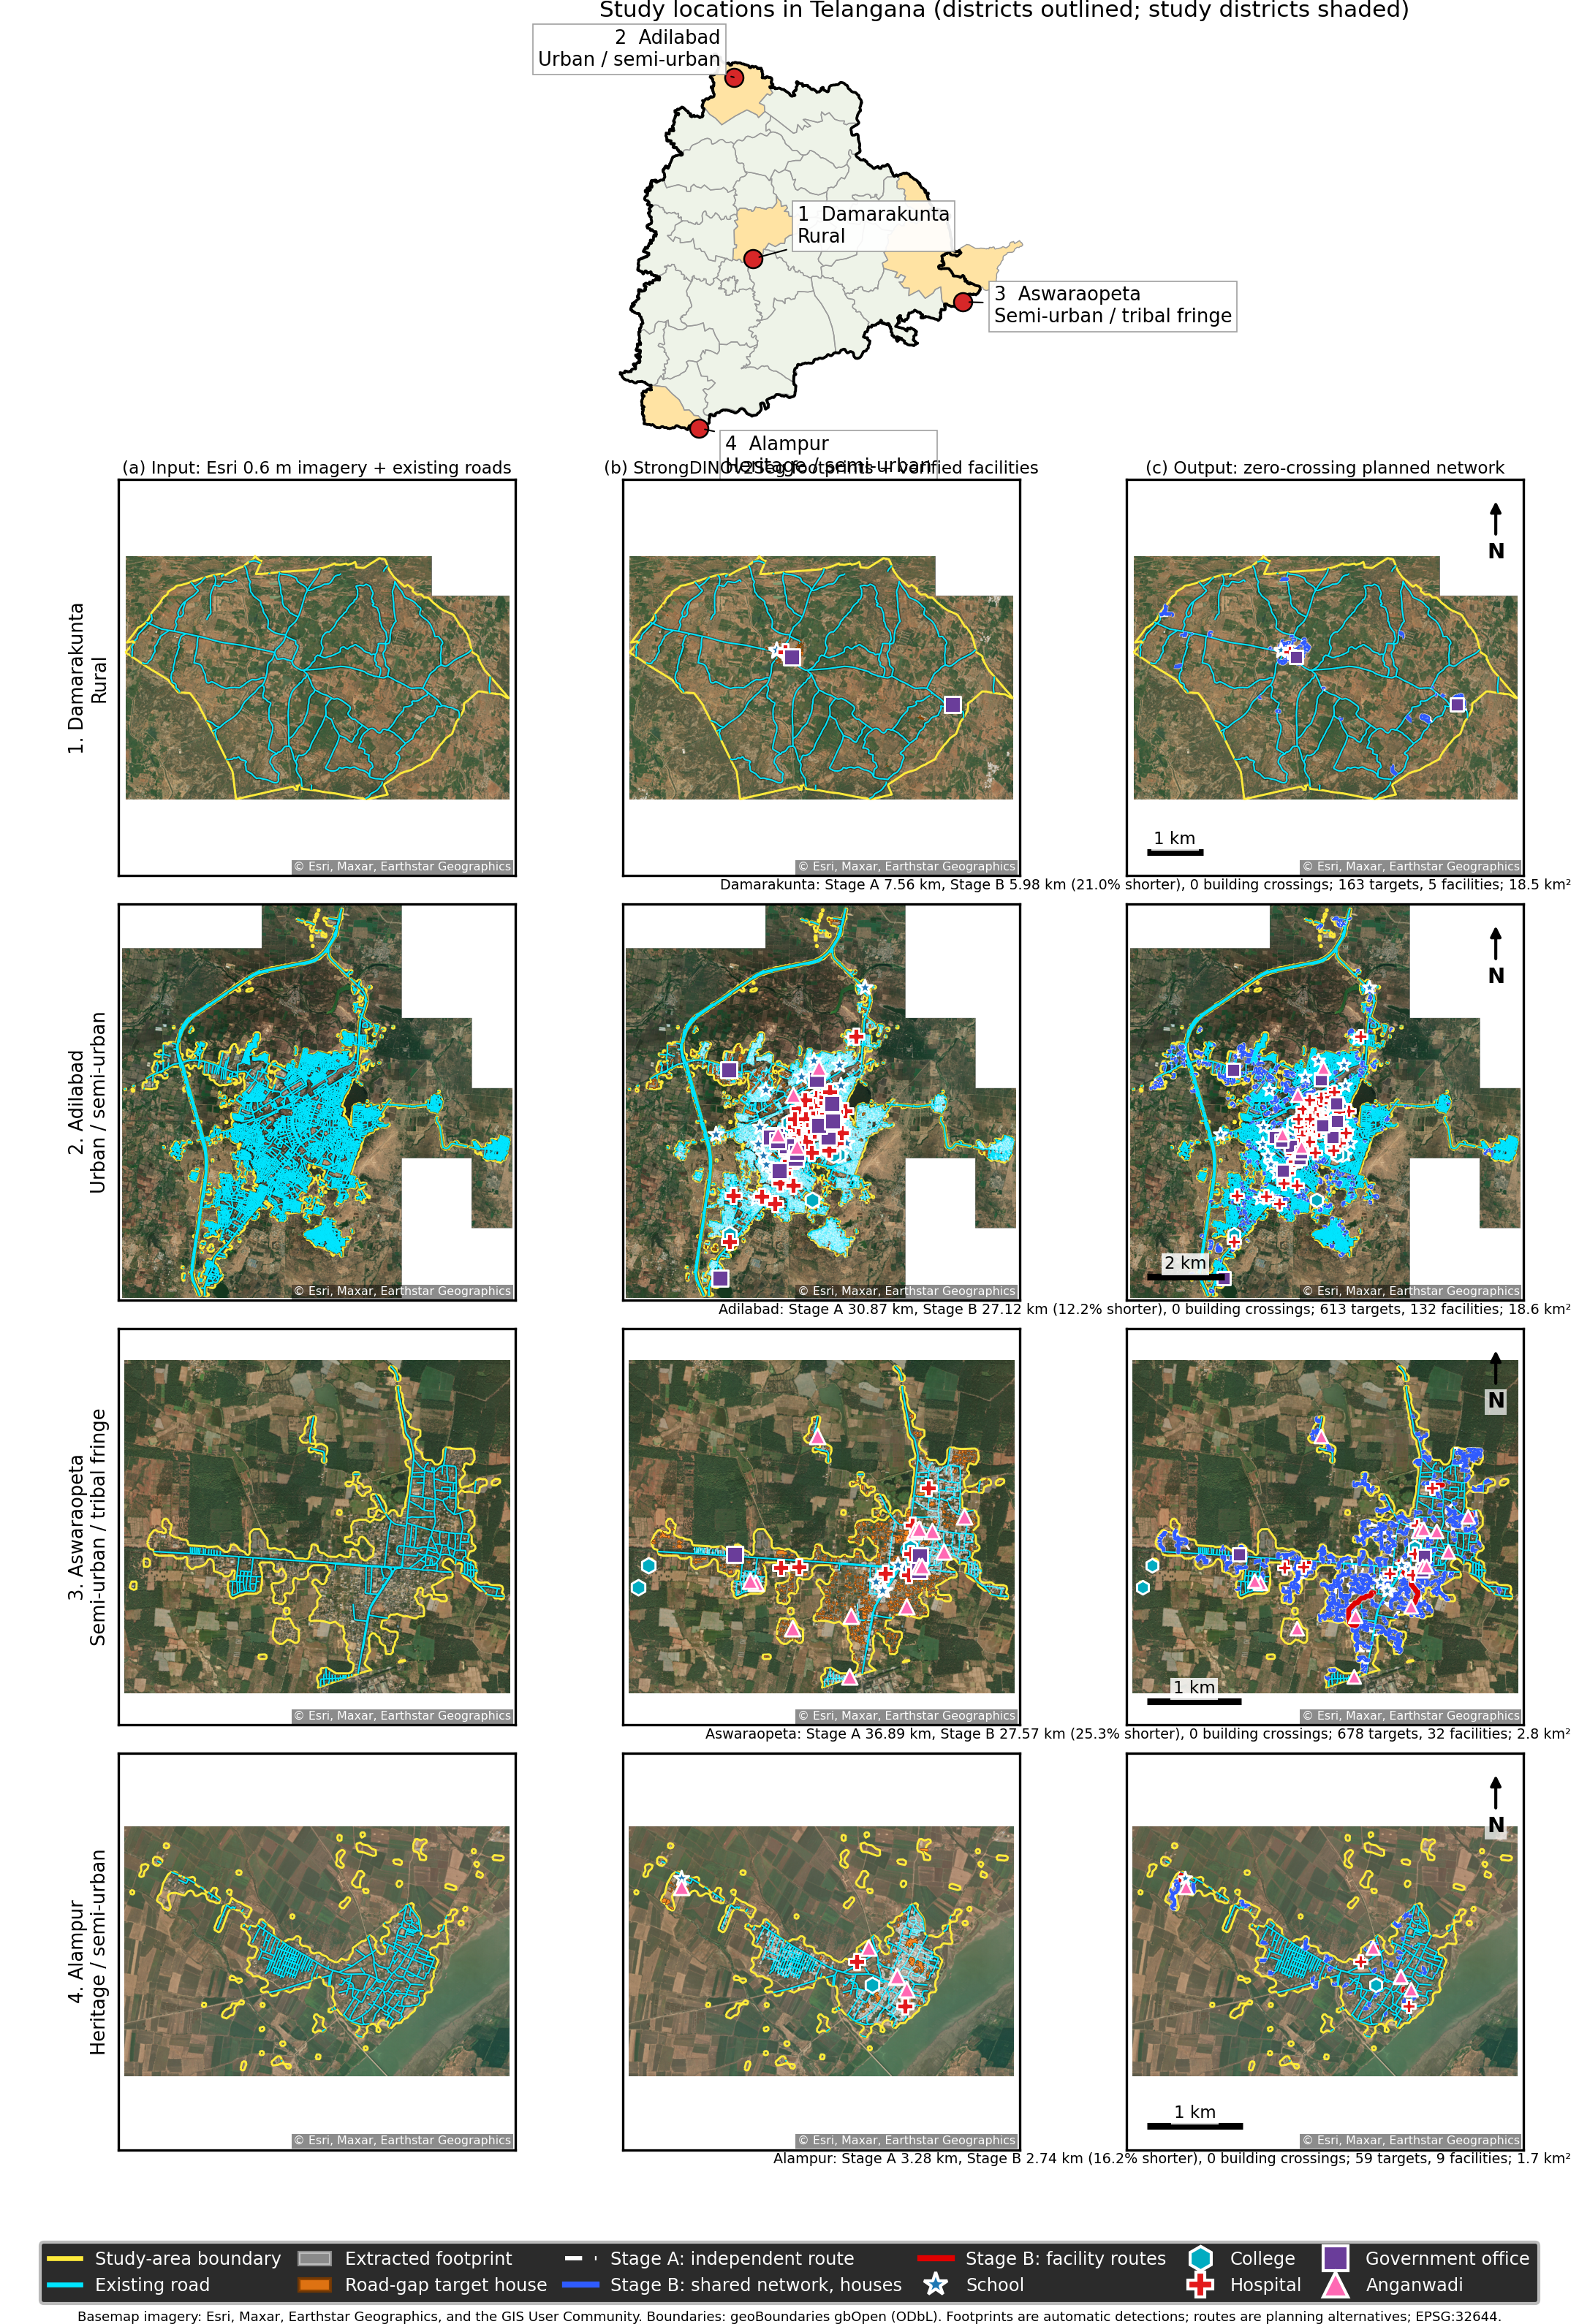
\includegraphics[width=0.93\textwidth]{figures/fig_flow_study_areas.png}}{\fbox{\parbox{0.8\textwidth}{\centering\pending{Figure not generated yet: run \texttt{python scripts/build\_paper\_flow\_figure.py --source segmentation} on the PC that holds the segmentation results.}}}}
\caption{Study areas and end-to-end flow. Top: Telangana with district outlines and the four study locations (1~Damarakunta, rural; 2~Adilabad, urban / semi-urban; 3~Aswaraopeta, semi-urban / tribal fringe; 4~Alampur, heritage / semi-urban). Rows 1--4: (a)~input, Esri World Imagery (0.6~m) with the existing road network; (b)~\dinoseg{} footprints (road-gap target houses in orange) with the verified facilities (School, College, Hospital, Government Office, Anganwadi); (c)~output, existing roads, Stage~A independent routes (white dashed) and Stage~B shared network (blue: houses; red: facilities) with the 5~m zero-crossing clearance, scale bar and north arrow. Basemap imagery: Esri, Maxar, Earthstar Geographics, and the GIS User Community. Footprints are automatic detections and routes are planning alternatives, not engineered roads.}
\label{fig:flow}
\end{figure*}

\begin{table*}[t]
\caption{Four study areas side by side. Segmentation rows: LoveDA validation of the single \dinoseg{} checkpoint (macro averages; F1-score equals the mean Dice). Routing rows: unique lengths on the 5~m zero-crossing grid (Stage~A independent, Stage~B shared network, shared edges once); building crossings are routes inside another building's footprint; the cost is the Stage~B length times Rs 75 lakh per km (range 60--90), an owner-supplied, unverified PMGSY-based rate, so it is illustrative and not an engineering estimate.}
\label{tab:four}
\centering
\scriptsize
\resizebox{\textwidth}{!}{\input{paper_comparison_table.tex}}
\end{table*}

\section{Discussion}
\subsection{What transfers and what does not}
The planning stages transferred without modification: the same cost surface, solver parameters and metrics produced connected plans in a dense window, both from \dinoseg{} footprints on Esri imagery (345 targets) and from open footprints (874 targets). The qualitative findings were reproduced in all three settings: sharing saves unique length (24.9\%, 14.7\% and 26.0\%), the footprint penalty trades length for exposure, and omissions shorten the plan while stranding households. What did not transfer is the benefit of the simpler baselines: roads-only sharing recovered most of the gain in the dispersed village (22.6\%) but almost none in the dense window (2.3\% and 2.9\%), which suggests that the value of a marginal-cost planner grows with settlement density, a hypothesis supported by one dense window. The two Adilabad footprint sources differ in the size of the saving (14.7\% against 26.0\%); with 57\% of the segmented instances being merged blocks, the segmentation result may reflect coarse, widely spaced targets, and no reference mask exists to say which footprint set is closer to the truth.

\subsection{Why pixel metrics are not enough for infrastructure use}
Segmentation metrics are area-weighted over classes, while the planner counts instances. A detector that misses the smallest quarter of buildings can lose few building pixels yet removes a quarter of households from the plan (table~\ref{tab:omission}), and a detector that merges adjacent roofs can score a high pixel IoU yet strands 38\% of the Damarakunta houses in the merged-blob scenario. Network length falls in both cases, so total length is a poor quality indicator. Merged blobs correspond to dense multi-roof structures; whether they coincide with the core of a hamlet was not measured.

\subsection{Land take and planning use}
Shared corridors reduce the length of new road for the same households. As an illustration only, assuming a 5~m formation width (an assumption of this study; no road-width data were available), the 1{,}684~m saved in Damarakunta corresponds to about 0.84~ha less land take, the 3{,}152~m saved in Adilabad (segmentation targets) to about 1.6~ha and the 12{,}060~m saved against the open-footprint targets to about 6.0~ha. For PMGSY-style schemes \cite{pmgsy} three points follow. Building inventories are uncertain inputs and a network sized from them should carry a sensitivity band. Shared corridors save about a quarter of unique length and this survives omissions. Local overrides should be used sparingly and documented. The outputs are screening-level alternatives; we do not claim compliance with Indian Roads Congress design standards, nor any engineering design value.

\subsection{Limitations}
(i) Two settlements only; the semi-urban and second rural windows are planned but have not been run. (ii) Omission scenarios are synthetic, not measured detection errors. (iii) Neither Damarakunta nor Adilabad has a surveyed reference mask; the LoveDA metrics come from the epoch-4 checkpoint with metadata recovered from the training notebook, and the checkpoint hash (SHA-256 \texttt{2e7c4646dc77ceb2\allowbreak a357f44f11cb3f7f\allowbreak f84e636871d70ba4\allowbreak c31e194e5ec00cf3}) was logged only for the Adilabad run, not with the Damarakunta candidates, although both runs loaded the same file path. (iv) In Adilabad 57\% of the \dinoseg{} instances are \textsc{Unresolved\_Merge} blocks, so its 345 targets are built-up units, not houses; the open footprints are map data of unverified completeness, and Overture licences were not re-verified. Ten of the 68 verified facility points share an identical coordinate with another Overture record (generic geocodes), so the 20 m footprint check is weak evidence in the dense fabric. (v) Costs are ordinal, the planner is a heuristic without an optimality guarantee, and road-gap targeting changes the problem, as the threshold sweep shows. (vi) Pixel accuracy is reported as 71.3\%, the value recomputed from the confusion matrix. (vii) Merged-blob and addition scenarios were run only for Damarakunta.

\section{Conclusions}
A pipeline from satellite imagery and open layers to shared access roads connects the houses and facilities of a rural village (24.9\% less unique corridor than independent routing) and, without changes to the cost surface or solver, those of an urban and peri-urban mandal, end to end on Esri imagery (14.7\% less) and on open footprints (26.0\% less). Footprint penalties and simulated inventory errors behave consistently in all three settings: penalties trade length for fewer routes through dwellings, and omissions shorten the plan while stranding households. The dependence of the roads-only baseline on settlement density, and the effect of detection quality across settings, are the main open questions; a semi-urban and a second rural window are planned to address the first.

\ifanon\else
\section*{Acknowledgments}
The authors acknowledge the Telangana State Remote Sensing Application Centre (TGRAC) for the boundary, road and facility layers of Damarakunta, and the providers of the open datasets used (ESA WorldCover, Copernicus DEM, Overture Maps, geoBoundaries, Google Open Buildings, LoveDA).
\fi

\section*{Data sources and imagery attribution}
High-resolution RGB satellite basemap imagery for Damarakunta Village and the Adilabad Urban window was obtained via Esri World Imagery (sources: Esri, Maxar, Earthstar Geographics, and the GIS User Community) and used strictly for non-commercial academic research and visual overlay in accordance with Esri's academic use terms, while raw imagery tiles are not redistributed. All derived modeling and multi-settlement planning layers rely on open-licensed datasets: ESA WorldCover 10~m v200 (CC BY 4.0), Copernicus GLO-30 DEM (Copernicus Open Access Licence), geoBoundaries ADM3 (ODbL 1.0), and Overture Maps (ODbL 1.0 / CDLA-Permissive-2.0). Damarakunta's boundary, road and facility layers are TGRAC data and its $\sim$30~m DEM source was not recorded; the Copernicus GLO-30 and geoBoundaries layers apply to the Adilabad window.

\section*{Funding}
This research received no specific grant from any funding agency in the public, commercial, or not-for-profit sectors.

\section*{Data availability statement}
\ifanon
Code, derived tables and the open-data manifests (with SHA-256 hashes) will be made available in a public repository on acceptance and are available to reviewers on request. TGRAC layers for Damarakunta are subject to the provider's terms.
\else
Code, derived summary tables, and the open-data manifests with SHA-256 hashes are available at \url{https://github.com/Archana519/Telangana-Rural-Project} (folders \path{DELIVERABLES_DAMARAKUNTA_STAGE_B} and \path{DELIVERABLES_CONTRIBUTION_3_MULTI_VILLAGE}, the latter including the Adilabad segmentation results in \path{01_ADILABAD_SEGMENTATION}). TGRAC layers for Damarakunta are subject to the provider's terms. The \dinoseg{} checkpoint is not included in the repository; its SHA-256 is given in Section~\ref{sec:methods}. A Zenodo DOI will be added when the archive is minted.
\fi

\section*{Conflict of interest}
The authors declare no competing interests.

\bibliographystyle{unsrt}
\bibliography{references}

\end{document}
"      (then bibtex / pdflatex as above)
% The IOP class (iopjournal / iopart) is not installed in this build environment, so the manuscript uses a plain
% `article` layout with the same logical front matter. At submission, paste the sections into the IOP journal
% template (Overleaf: "IOP journal article template", option [anonymous] for double-anonymous review).
% Every number in Sections 3-5 is checked by paper_eris/verify_eris_numbers.py against
% DELIVERABLES_DAMARAKUNTA_STAGE_B/ and DELIVERABLES_CONTRIBUTION_3_MULTI_VILLAGE/01_ADILABAD/.
% =============================================================================================================
\documentclass[12pt,a4paper]{article}
\usepackage[margin=2.5cm]{geometry}
\usepackage{setspace}\onehalfspacing
\usepackage{graphicx}
\usepackage{booktabs}
\usepackage{array}
\usepackage{amsmath,amssymb}
\usepackage{url}
\usepackage{xcolor}
\usepackage{algorithm}
\usepackage{algpseudocode}
\usepackage[hidelinks]{hyperref}
\setlength{\emergencystretch}{3em}
\newif\ifanon
\ifdefined\ANON\anontrue\fi
\newcommand{\dinoseg}{StrongDINOv2Seg}
\newcommand{\Lcost}{L_{\mathrm{cost}}}
\newcommand{\pending}[1]{\textcolor{red}{\textit{#1}}}% value not yet computed on the machine that generated paper_comparison_table.tex
\algrenewcommand\algorithmicrequire{\textbf{Input:}}
\algrenewcommand\algorithmicensure{\textbf{Output:}}

\begin{document}

\begin{center}
{\Large\bfseries Smart village infrastructure planning and road network optimization for rural Telangana\par}
\vspace{0.8em}
\ifanon
{\large [Authors withheld for double-anonymous review]\par}
\else
\small\begin{tabular}{@{}p{0.47\textwidth}p{0.47\textwidth}@{}}
\centering\textbf{Ramakrishna Kolikipogu}\par
\centering\textit{Department of Information Technology}\par
\centering\textit{Chaitanya Bharathi Institute of Technology (A)}\par
\centering Hyderabad, India\par
\centering krkrishna.cse@gmail.com\par
&
\centering\textbf{Pendyala Archana}\par
\centering\textit{Department of Information Technology}\par
\centering\textit{Chaitanya Bharathi Institute of Technology (A)}\par
\centering Hyderabad, India\par
\centering pendyalaarchanareddy98@gmail.com\par
\end{tabular}\\[1.4em]
\fi
\end{center}

\begin{abstract}
\noindent Rural road infrastructure planning faces several challenges, including incomplete spatial data, unplanned settlements, difficult terrain, and limited information about suitable road connections to essential public services such as hospitals, schools, and government institutions. Conventional road-planning approaches often rely on manual decision-making and shortest-path algorithms, which may not adequately consider the influence of spatial-data errors, terrain conditions, land-use constraints, and opportunities for sharing road segments. To address these challenges, this work proposes an AI- and GIS-based framework for rural village infrastructure planning and road-network optimization. The proposed framework integrates high-resolution satellite imagery, existing road-network data, village boundary information, land-cover maps, elevation data, and public-service locations. A StrongDINOv2Seg deep-learning model is employed for semantic segmentation, supported by GIS-based feature extraction to identify relevant spatial features. A multi-criteria cost surface is then generated by considering land-cover conditions, terrain slope, and restricted areas to identify suitable movement paths. For road-network planning, a two-stage approach is implemented: in the first stage, alternative least-cost routes are generated using grid-based Dijkstra pathfinding; in the second stage, a greedy shared-network selection strategy evaluates alternative routes based on their marginal cost and gives credit to road segments already included in the selected network, reducing unnecessary route duplication while prioritizing connections to public-service facilities and residential buildings. The framework is demonstrated on Damarakunta village in Siddipet District, Telangana, and evaluated for cross-morphology transferability in Adilabad Urban. On the LoveDA validation benchmark, the segmentation model achieved a mean Intersection over Union (mIoU) of 53.8\% and a mean Dice score of 68.9\%. In the Damarakunta building-access planning experiment, the two-stage network-aware approach produced 5{,}069.0~m of unique route length compared with 6{,}753.1~m for independent least-cost routing, representing a reduction of 24.9\%. Re-applied end to end to Adilabad Urban on Esri imagery, the same cost surface and solver reduced unique route length from 21{,}440.8~m to 18{,}288.7~m (14.7\%) for 345 road-gap targets, and with open Overture Maps footprints from 46{,}419.2~m to 34{,}358.8~m (26.0\%), confirming consistent network-sharing behavior across contrasting settlement densities, although a roads-only shared reference recovered most of the saving in Damarakunta (22.6\%) but little in Adilabad (2.3\% and 2.9\%). Because most StrongDINOv2Seg instances in Adilabad's dense fabric are merged roof blocks, its targets are built-up units rather than counted houses. The proposed framework provides a GIS-based decision-support approach for analyzing rural infrastructure requirements and generating cost-aware road-network alternatives as computational planning suggestions requiring field validation prior to implementation.
\end{abstract}

\noindent\textit{Keywords}: rural roads, building footprint extraction, satellite remote sensing, least-cost path, shared network, spatial transferability, open geospatial data, Telangana

\section{Introduction}
Road building is among the most consequential land-use changes of the coming decades. Global road length is projected to grow by roughly 3.0--4.7 million km by 2050 \cite{meijer2018global}, and new roads open land to clearing, fragmentation and conversion \cite{laurance2014global}. Much of this growth is local. In India the Pradhan Mantri Gram Sadak Yojana (PMGSY) connects habitations through all-weather rural roads \cite{pmgsy}, and planning for such schemes depends on knowing where dwellings and facilities are, what terrain and land cover a corridor must cross, and which connection rule is applied.

Computational support for this planning has matured along three separate lines. Remote sensing now maps buildings and roads at large scale, from continental building inventories \cite{sirko2021openbuildings} to foundation-model segmenters \cite{oquab2023dinov2}, with recent work addressing small and isolated rural buildings, uncertainty, and domain shift \cite{r62,r63,r64,r65,r66,r67,r68,r69,r70}. Multi-criteria and least-cost analysis translates terrain and land cover into route costs \cite{r06,r53,r54,collischonn2000lcp}. Network-design formulations connect many demand points at low total cost, including Steiner-tree heuristics \cite{kou1981steiner,mehlhorn1988steiner,hwang1992steiner,r51}, rural road design models \cite{r41,r43,r44} and recent analogues for power and transport networks \cite{r45,r46,r47,r50}. These lines are rarely joined: detectors are judged by pixel overlap \cite{r01}, planners assume an error-free inventory, and each house is often connected independently, so neighbouring houses re-trace the same corridor.

We join them in a single reproducible pipeline and test it at two settlement densities. Our contributions are:
\begin{enumerate}
\item \textbf{End-to-end pipeline.} A pipeline from satellite imagery to a shared access network: StrongDINOv2Seg segmentation, OpenCV/NumPy distance-transform instance extraction with an explicit merge flag, a multi-criteria cost surface with a footprint penalty, and a two-stage shared-network planner (Section~\ref{sec:methods}).
\item \textbf{Error propagation.} Controlled omission and addition scenarios that propagate building-inventory errors through the planner, measuring their effect on unique length, coverage and exposure of dwellings (Sections~\ref{sec:damar}--\ref{sec:adilabad}).
\item \textbf{Multi-settlement spatial transferability and open-data scalability.} The rural Damarakunta workflow is re-applied, with the same cost-surface definition and solver, to the Adilabad Urban mandal (urban and peri-urban): end to end on Esri imagery (StrongDINOv2Seg and instance extraction) and, as an independent check, on open Overture Maps footprints, with a road-gap rule for targets and robustness examined over penalty settings, road-gap thresholds and synthetic omissions (Section~\ref{sec:adilabad}).
\end{enumerate}
Two scope limits apply. Only these two settlements were evaluated; a semi-urban and a second rural window are planned but not yet run, so we make no claim about a full rural--semi-urban--urban gradient. And the Adilabad segmentation results are unvalidated: no reference building mask exists, and in the dense fabric most detected instances are merged roof blocks (Section~\ref{sec:adilabad}), so the Adilabad targets are built-up units rather than counted houses.

\section{Related work}
\textbf{Building extraction.} Reviews of building extraction from remote sensing \cite{r01} document the shift from fully convolutional networks \cite{ji2019whu} to transformer and foundation-model encoders. Recent studies target isolated small buildings \cite{r63}, weak supervision \cite{r62}, uncertainty-guided refinement \cite{r64,r65}, and domain generalisation or adaptation across imagery sources \cite{r02,r66,r67,r68,r69,r70}. Road extraction has followed the same path, with width-adaptive, topology-preserving and foundation-model-based networks for rural and arid scenes \cite{r56,r57,r58,r59,r60}, and topological analysis has been used to detect informal settlements worldwide \cite{r48}. Evaluation is overwhelmingly through overlap scores on benchmark data \cite{foody2002status}; the effect of detection errors on downstream infrastructure decisions is rarely quantified, although error propagation in GIS models is long established \cite{heuvelink1998error}.

\textbf{Route and network planning.} Multi-criteria GIS analysis \cite{r06} and least-cost path methods \cite{collischonn2000lcp,r53,r54} underlie corridor selection for roads, with dedicated treatments of slope \cite{r54}, route alternatives \cite{r53} and travel-time uncertainty \cite{r61}, and GIS route reconstruction has been applied to historical transport routes \cite{r55}. Rural road design has been addressed with improved network-design models \cite{r41}, algorithmic planning under constrained capacities in India \cite{r43} and facility-based methodology \cite{r44}. Steiner-tree formulations \cite{hwang1992steiner} and their shortest-path-based heuristics \cite{kou1981steiner,mehlhorn1988steiner} connect many terminals at low total length and are applied to sub-network identification \cite{r51}, multi-terminal routing \cite{r52}, cable routing \cite{r45}, minimum spanning trees of road networks \cite{r46}, rural grids \cite{r47} and least-cost electrification \cite{r50}.

\textbf{Gap.} To our knowledge no cited work combines (i) satellite-derived building instances, (ii) a land-cover- and slope-based cost surface with building avoidance, (iii) a shared-network planner whose marginal cost credits built corridors, and (iv) a systematic test of how inventory omissions and the settlement setting change the result. This paper addresses that combination for rural Telangana and treats the comparison between two settlements as an explicit transferability test.

\section{Study areas and data}
\subsection{Damarakunta (rural)}
Damarakunta is a rural revenue village in Markook mandal, Siddipet district, Telangana ($\approx 17.707^{\circ}$N, $78.753^{\circ}$E). Its boundary, from the Telangana State Remote Sensing Application Centre (TGRAC), encloses 18.47~km$^2$ (UTM zone 44N, EPSG:32644; figure~\ref{fig:flow}). Settlement is dispersed, with small house clusters separated by farmland. A 0.6~m, three-band mosaic (11{,}296 $\times$ 7{,}171 px) was assembled from Esri World Imagery exports. Building candidates are model outputs: 278 polygons, 165 inside the boundary, of which 163 are used as routing targets. They carry a quality class: \textsc{Plausible} (71), \textsc{Review} (32) and \textsc{Unresolved\_Merge} (62), the last denoting blobs that merge adjacent roofs and could not be split. Five TGRAC facilities (schools, a health sub-centre and the gram-panchayat headquarters points) are planned in a separate phase. No ground-truth building mask exists for Damarakunta.

\subsection{Adilabad Urban (urban and peri-urban)}\label{sec:adilabad_data}
The second window is the Adilabad Urban mandal, Adilabad district (geoBoundaries ADM3 polygon; centroid $19.682^{\circ}$N, $78.528^{\circ}$E), 17.75~km$^2$, close to Damarakunta in area. The 10~m grid has 424 $\times$ 564 cells, 177{,}533 of them inside the polygon, 0.62\% blocked (water or slope $>25^{\circ}$). About 60\% of cells are not WorldCover built-up, so the window holds an urban core and a peri-urban fringe. The boundary layer is the 2018 release and may differ from current municipal limits.

Two sets of building footprints are used. (i)~\emph{Segmentation footprints (primary, end to end).} A 0.6~m Esri World Imagery mosaic of the window (7{,}248 $\times$ 9{,}590~px, EPSG:32644) was exported with the Damarakunta recipe (1{,}800~m tiles). \dinoseg{} was applied to 391 tiles of $560\times560$~px (stride 420~px, margin 70~px, the Damarakunta tiling; Damarakunta: 459 tiles) and the same instance extraction. This yields 2{,}769 instances, of which 2{,}690 have an area of at least 30~m$^2$ and form the penalty layer; their quality classes are \textsc{Plausible} (1{,}033), \textsc{Review} (77) and \textsc{Unresolved\_Merge} (1{,}580), the last with a median area of 1{,}125.5~m$^2$ (\textsc{Plausible}: 207.4~m$^2$). Of 83 Overture place candidates inside the window, 68 are verified with the Damarakunta rule (a detected footprint within 20~m): 44 schools, 20 health and 4 government. (ii)~\emph{Open footprints (independent check).} Overture release 2026-10-21.0 \cite{overture2026} supplies 4{,}850 road segments, 24{,}924 building polygons (18{,}846 from OpenStreetMap, 6{,}078 from Google Open Buildings v3 \cite{sirko2021openbuildings}) and 738 places; footprints with area $\ge 30$~m$^2$ and confidence $\ge 0.7$ (18{,}242 polygons) form the penalty layer, and 71 of the 83 facility candidates are verified (44 schools, 20 health, 7 government) after manual removal of mis-geocoded records. Roads are Overture/OSM segments in both variants (table~\ref{tab:data}). Neither footprint set has been field-verified. Figure~\ref{fig:flow} shows the study window, the detected footprints and the verified facilities of every study area.

\begin{table}[t]
\caption{Input data and licence status. ``Not re-verified'' marks Overture licences taken from the provider documentation, which could not be opened from the execution environment.}
\label{tab:data}
\centering
\footnotesize
\begin{tabular}{@{}>{\raggedright\arraybackslash}p{3.0cm}>{\raggedright\arraybackslash}p{5.9cm}>{\raggedright\arraybackslash}p{5.5cm}@{}}
\toprule
Layer & Damarakunta / Adilabad source & Licence status \\
\midrule
Boundary & TGRAC polygon / geoBoundaries ADM3 \cite{runfola2020geoboundaries} & TGRAC: not stated / ODbL 1.0 \\
Roads, facilities & TGRAC (43 road features, 5 facilities) / Overture Maps 2026-10-21.0 \cite{overture2026} & TGRAC: not stated / ODbL 1.0 (roads), CDLA-Permissive-2.0 (places); not re-verified \\
Buildings & StrongDINOv2Seg instances (0.6~m Esri imagery; both windows) / Overture footprints (Adilabad check; OSM, Google Open Buildings v3 \cite{sirko2021openbuildings}) & Esri academic-use terms, tiles not redistributed / ODbL 1.0 and CC BY 4.0; not re-verified \\
Land cover & ESA WorldCover v200, 10~m \cite{zanaga2021worldcover} & CC BY 4.0 \\
Terrain & $\sim$30~m DEM (source not recorded) / Copernicus GLO-30 \cite{esa2022copdem}; Sobel slope, bilinear to 10~m & Not stated / Copernicus Open Access Licence \\
Training benchmark & LoveDA \cite{wang2021loveda} & Source domain only \\
\bottomrule
\end{tabular}
\end{table}

\section{Methods}\label{sec:methods}
The framework is a seven-step chain (figure~\ref{fig:arch}): (1)~multi-source open-data ingestion (Esri World Imagery, ESA WorldCover, Copernicus GLO-30, Overture / OSM / TGRAC roads, the study polygon); (2)~\dinoseg{} semantic segmentation in 560~px tiles; (3)~distance-transform extraction of building footprints and road-gap targets; (4)~a four-pass multi-source facility audit that snaps every facility onto a roof; (5)~a multi-criteria cost surface with a 5~m zero-crossing building clearance; (6)~Stage~A and Stage~B Dijkstra shared-network routing; and (7)~connectivity and PMGSY-based cost evaluation. Steps 1 to 7 are identical for all four study areas; the settlements differ only in their inputs. The ten-metre soft-penalty planner of the earlier experiments is kept as a comparison baseline (section~\ref{sec:damar}), and the clearance network is the proposed plan (section~\ref{sec:four}).

\begin{figure}[t]
\centering
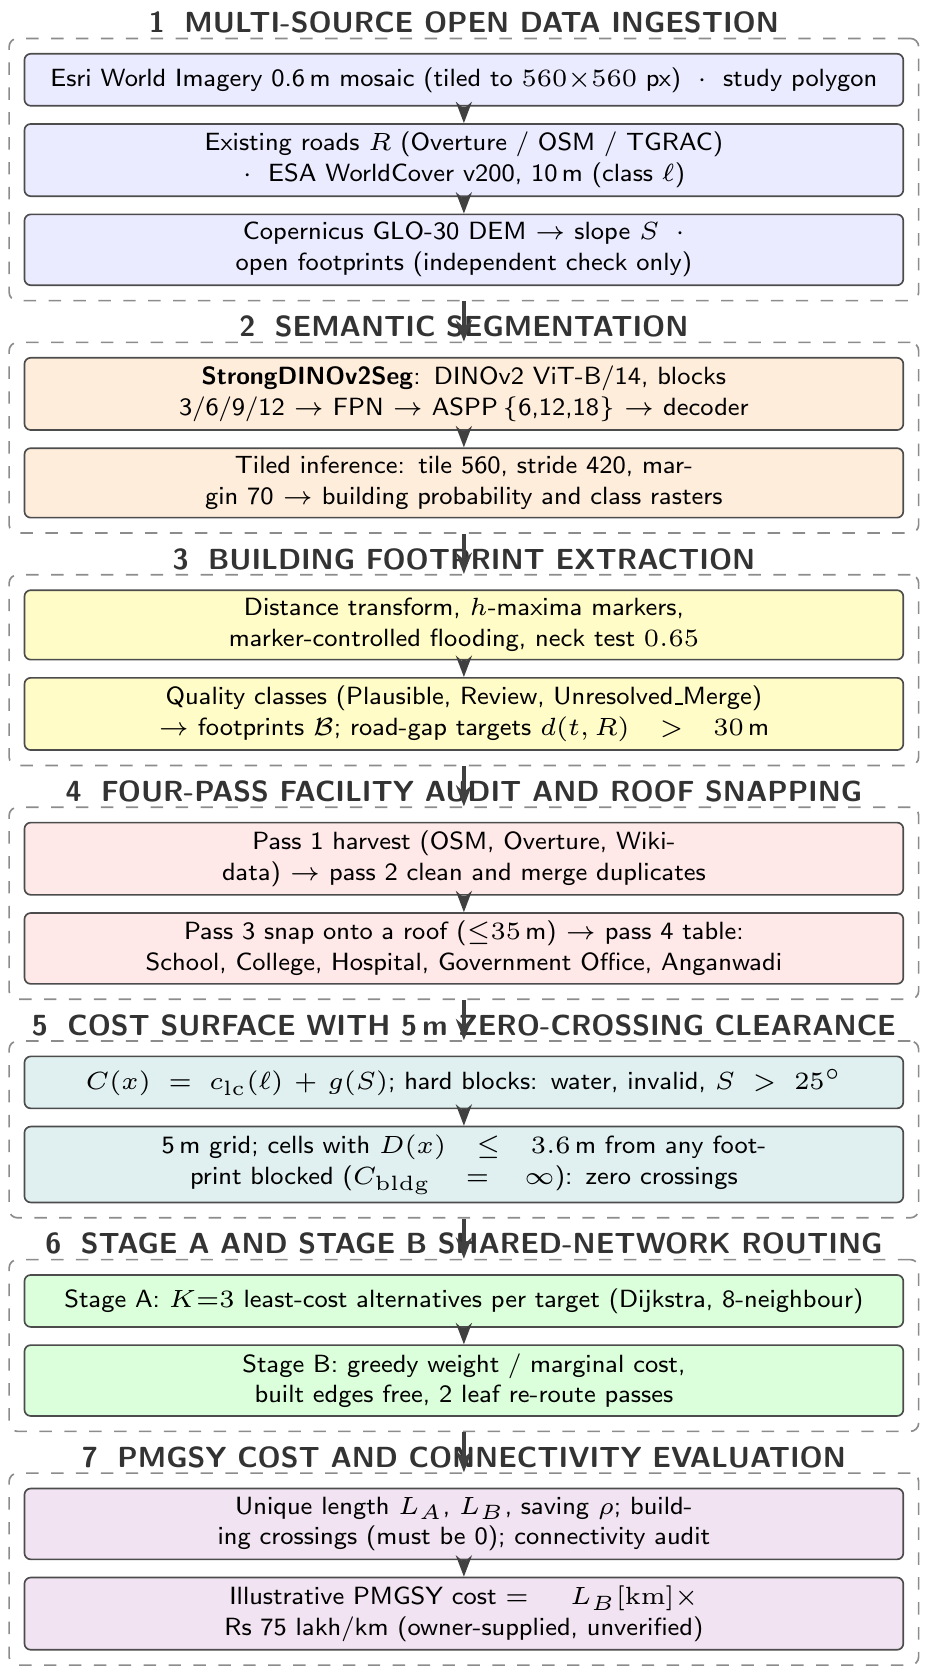
\includegraphics[width=0.5\textwidth]{figures/fig_architecture.png}
\caption{Seven-step architecture: (1)~multi-source open-data ingestion, (2)~\dinoseg{} semantic segmentation (tile 560, stride 420, margin 70), (3)~distance-transform building footprint extraction (neck ratio 0.65), (4)~four-pass multi-source facility audit and roof snapping (School, College, Hospital, Government Office, Anganwadi), (5)~cost surface with a 5~m zero-crossing clearance (3.6~m), (6)~Stage~A independent and Stage~B shared-network Dijkstra routing, (7)~PMGSY cost and connectivity evaluation.}
\label{fig:arch}
\end{figure}

\subsection{Building extraction}
\dinoseg{} is a fully fine-tuned DINOv2 ViT-B/14 encoder \cite{oquab2023dinov2}. Tokens from blocks 3, 6, 9 and 12 are projected to 256 channels, fused (FPN-style \cite{lin2017fpn}), passed through an ASPP neck (rates 6, 12, 18) \cite{chen2018deeplabv3plus} and a four-stage decoder with auxiliary heads for deep supervision \cite{lee2015dsn}. Training used LoveDA \cite{wang2021loveda} at 560~px for a scheduled 10 epochs (AdamW, cosine schedule to $10^{-7}$, encoder learning rate $\times 0.1$) with loss $0.5\,\mathrm{CE}+0.4\,\mathrm{Dice}+0.1\,\mathrm{edge}$ \cite{milletari2016vnet} and auxiliary weight 0.4. The epoch-4 checkpoint was used; the file used for the Adilabad run has SHA-256 \texttt{2e7c4646dc77ceb2\allowbreak a357f44f11cb3f7f\allowbreak f84e636871d70ba4\allowbreak c31e194e5ec00cf3}. Building instances are extracted from the predicted mask with OpenCV and NumPy: h-maxima of the distance transform give markers, a neck test (ratio 0.65) decides whether touching blobs are split, and blobs that cannot be split are flagged \textsc{Unresolved\_Merge}.

\subsection{Road-gap targets and Adilabad footprint sources}
For Adilabad the same imagery-to-footprint chain is run on Esri imagery (Section~\ref{sec:adilabad_data}), and Overture footprints serve as an independent check. Because connecting every footprint is meaningless in a built-up fabric already served by roads, only houses more than 30~m (the planner snap distance) from an existing road are routed. Planner cost grows roughly quadratically with the number of targets, which further motivates the filter; the threshold is varied (20, 30, 50~m) in Section~\ref{sec:adilabad}.

\subsection{Cost surface}
Let $\mathcal{B}$ be blocked cells (water, invalid cells, slope $>25^{\circ}$) and $\mathcal{P}$ the cells whose centre lies inside a footprint. The graph has the unblocked 10~m cells as nodes and 8-neighbour edges with no diagonal corner-cutting. The cell cost is
\begin{equation}
c(x)=\bigl[c_{\mathrm{lc}}(\ell(x))+g(s(x))\bigr]\,m(x),\qquad m(x)=\begin{cases}\mu & x\in\mathcal{P}\\ 1 & \text{otherwise,}\end{cases}
\label{eq:cell}
\end{equation}
where $\ell$ is the WorldCover class with resistance $c_{\mathrm{lc}}=8,5,3,6,2,4$ for trees, shrubland, grassland, cropland, built-up and bare/sparse land respectively (classes 10--60 in the order 10, 20, 30, 40, 50, 60), $g(s)=4\,\mathrm{clip}(s,0,10)/10$ with $s$ the slope in degrees, and $\mu=4$ is the footprint penalty. Edge weights are the mean end-cell cost times step length. Costs are ordinal planning units, not currency. In Damarakunta the penalty is lifted within a 20~m disc around the health sub-centre,  The land-cover, slope, cost and blocked-cell rasters are the inputs of the cost surface of every study area (figure~\ref{fig:flow}).whose point lies on the edge of its own footprint.

\subsection{Shared-network planner}
For each target, Stage~A computes a least-cost path to the existing road cells with Dijkstra's algorithm \cite{dijkstra1959note,hart1968astar,collischonn2000lcp} and alternatives by inflating costs along earlier paths ($K=3$ alternatives in total). Stage~B greedily selects the (target, alternative) pair with the highest weight per marginal cost
\begin{equation}
\Delta\Lcost\bigl(\pi\mid S\bigr)=\sum_{e\in\pi\setminus E_S}w(e),
\label{eq:marginal}
\end{equation}
where $E_S$ is the set of already selected edges, so built edges are free and a route may end on another route. This is the shortest-path heuristic for Steiner trees \cite{kou1981steiner,mehlhorn1988steiner} on a penalised, land-cover-weighted graph with the road network as a free sub-tree; it carries no optimality guarantee. Two passes of leaf re-routing follow. Snap distance is 30~m, search limit 1{,}500~m and attachment tolerance 15~m. Facilities are planned in a separate phase.

\subsection{Facility audit and roof snapping}
Overture Places alone mislocated or missed colleges, hospitals, offices and anganwadis, so the facilities of each area come from a four-pass audit (\texttt{scripts/audit\_facilities.py}). Pass~1 harvests candidates inside and within 500~m of the polygon from OpenStreetMap (Overpass and the Photon geocoder), Overture Places, Wikidata and Wikipedia (and, for Damarakunta, the TGRAC layers); LGD, UDISE+ and the district directories have no open query interface and were not used. Pass~2 assigns one of five categories (School, College, Hospital, Government Office, Anganwadi), removes closed or commercial records (pharmacies, laboratories, coaching centres, banks, cooperative societies), religious sites, foreign place names, placeholder coordinates shared by several differently named records, and merges duplicates of one campus across sources; every removal is logged with its reason. Pass~3 moves each survivor onto the footprint that contains it or, failing that, the nearest footprint of at least 25~m$^2$ within 35~m (a compound building up to 25~m away for a school, college or hospital), and removes facilities with no building in range. Pass~4 writes the verified table with the sources, the snap distance and a confidence label; records with a single source and a snap of more than 12~m are kept with \texttt{use\_in\_analysis}${}=$\,False and are not routed.

\subsection{Zero-crossing building clearance}
The soft footprint penalty $\mu$ in equation~\ref{eq:cell} lets a route cross a roof when the detour costs more. The proposed plan therefore uses a hard barrier on a finer grid. Each 10~m cost cell is refined to $2\times2$ cells of cell size $\Delta=5$~m with the same cost per metre, and every cell whose centre lies within $r_c=3.6$~m of any footprint is blocked (equation~\ref{eq:bldg}). Because $r_c>\Delta\sqrt2/2=3.54$~m, no step between two free cell centres can touch a footprint: a point of the step lies within $\Delta\sqrt2/2$ of one of its end points, and that end point would then have been blocked. A target sits inside its own building, so each route starts at the edge of that building and reaches the nearest free cell that is connected to the road network by a straight lane of at most the snap distance that touches no other footprint; a target with no such lane (a house enclosed by other buildings) is reported as unrouted, never routed over a roof. Lengths are measured from the building edge. Every drawn route (lane, path and attachment to a road) is finally intersected with all footprints other than its own.

\subsection{Mathematical formulation}
\paragraph{Segmentation loss.} With logits $\mathbf z$, labels $y$, class probabilities $p_{ic}$ and one-hot targets $t_{ic}$ at pixel $i$ (class 0 is ignored),
\begin{equation}
\mathcal L(\mathbf z,y)=0.5\,\mathcal L_{\mathrm{CE}}+0.4\,\mathcal L_{\mathrm{Dice}}+0.1\,\mathcal L_{\mathrm{edge}},\qquad
\mathcal L_{\mathrm{total}}=\mathcal L(\mathbf z^{\mathrm{main}},y)+0.4\sum_{j=1}^{3}\mathcal L(\mathbf z^{(j)},y),
\label{eq:loss}
\end{equation}
\begin{equation}
\mathcal L_{\mathrm{Dice}}=\frac1{|\mathcal C|}\sum_{c\in\mathcal C}\Bigl(1-\frac{2\sum_i p_{ic}t_{ic}+\varepsilon}{\sum_i p_{ic}+\sum_i t_{ic}+\varepsilon}\Bigr),\qquad
\mathcal L_{\mathrm{edge}}=\frac1{|\Omega|}\sum_{i\in\Omega}(1+4e_i)\,\mathrm{CE}_i,\quad e_i=\min\{1,\,|(K_x{*}y)_i|+|(K_y{*}y)_i|\}.
\label{eq:diceedge}
\end{equation}
Here $\mathcal C$ is the set of scored classes, $\varepsilon$ a small smoothing constant, $K_x,K_y$ the Sobel kernels, so that the edge term up-weights the cross-entropy of pixels on label boundaries by up to five; the three auxiliary heads $\mathbf z^{(j)}$ provide deep supervision.

\paragraph{Evaluation metrics.} From the confusion matrix, with $TP_c,FP_c,FN_c$ the true positives, false positives and false negatives of class $c$ and $N$ the number of labelled pixels,
\begin{equation}
\mathrm{OA}=\frac{\sum_c TP_c}{N},\quad P_c=\frac{TP_c}{TP_c+FP_c},\quad R_c=\frac{TP_c}{TP_c+FN_c},\quad F_{1,c}=\frac{2P_cR_c}{P_c+R_c}=\frac{2TP_c}{2TP_c+FP_c+FN_c},\quad \mathrm{IoU}_c=\frac{TP_c}{TP_c+FP_c+FN_c},
\label{eq:metrics}
\end{equation}
and $P$, $R$, $F_1$ (the Dice coefficient) and $\mathrm{mIoU}=|\mathcal C|^{-1}\sum_{c\in\mathcal C}\mathrm{IoU}_c$ are the macro averages over the scored classes. Because $F_{1,c}$ equals the per-class Dice score, the reported F1-score is the mean Dice.

\paragraph{Terrain.} Slope is taken from the Copernicus GLO-30 elevation $z$ with the Sobel gradient at the DEM spacing $\Delta_z=30$~m, resampled bilinearly to the planning grid:
\begin{equation}
\partial_x z\approx\frac{(K_x{*}z)}{8\Delta_z},\quad \partial_y z\approx-\frac{(K_y{*}z)}{8\Delta_z},\quad S=\arctan\sqrt{(\partial_x z)^2+(\partial_y z)^2},\quad p_S=100\tan S,
\label{eq:slope}
\end{equation}
with $S$ the slope in degrees and $p_S$ the equivalent percentage slope reported in the comparison table. The cost uses the linear ramp $g(S)=w_s\min(S,S_{\mathrm{ref}})/S_{\mathrm{ref}}$ with $w_s=4$ and $S_{\mathrm{ref}}=10^{\circ}$, and cells with $S>S_{\lim}=25^{\circ}$ are blocked; no separate IRC slope-penalty factor is applied.

\paragraph{Composite cost and clearance barrier.} With $c_{\mathrm{lc}}(\ell)$ the WorldCover resistance (equation~\ref{eq:cell}, so the land-cover weight is $w_{\mathrm{lc}}=1$) and $D(x)$ the Euclidean distance from the centre of cell $x$ to the nearest footprint (zero inside a footprint),
\begin{equation}
C(x)=c_{\mathrm{lc}}(\ell(x))+g(S(x))+C_{\mathrm{bldg}}(x),\qquad C_{\mathrm{bldg}}(x)=\begin{cases}\infty & D(x)\le r_c\\ 0 & \text{otherwise,}\end{cases}\qquad r_c=3.6\ \mathrm{m},\ \Delta=5\ \mathrm{m}.
\label{eq:bldg}
\end{equation}
The ten-metre comparison baseline instead multiplies the cost of cells whose centre lies in a footprint by $\mu=4$ (equation~\ref{eq:cell}).

\paragraph{Graph and routing objectives.} The graph has the free cells as nodes and 8-neighbour edges, a diagonal step being allowed only if both orthogonal neighbours are free. The weight of an edge $(u,v)$ is
\begin{equation}
w(u,v)=d(u,v)\,\frac{C(u)+C(v)}{2},\qquad d(u,v)=\begin{cases}\Delta&\text{cardinal step}\\ \sqrt2\,\Delta&\text{diagonal step.}\end{cases}
\label{eq:edge}
\end{equation}
Stage~A gives every target $t$ the independent least-cost path $\pi_t^{A}=\arg\min_{\pi:\,t\to R}\sum_{e\in\pi}w(e)$ to the existing road cells $R$ (Dijkstra), and two further alternatives that multiply $w(e)$ by $\lambda\in\{3,8\}$ on cells within $20$~m of the earlier paths and overlap them by at most 80\%. Stage~B starts from $E_S=\emptyset$ and repeatedly serves the target and route with the highest weight per marginal cost,
\begin{equation}
(t^\star,\pi^\star)=\arg\max_{t\in U,\ \pi\in\Pi_t\cup\{\pi_t^{\mathrm{net}}\}}\frac{\omega_t}{\Delta\Lcost(\pi\mid S)},\qquad
\Delta\Lcost(\pi\mid S)=\sum_{e\in\pi\setminus E_S}w(e),
\label{eq:stageb}
\end{equation}
where $U$ is the set of unserved targets, $\Pi_t$ the Stage~A alternatives, $\pi_t^{\mathrm{net}}$ the least-cost path to the roads together with the routes already selected, and $\omega_t$ the priority weight ($4$ for hospitals and health centres, $3$ for schools, colleges and anganwadis, $2$ for government offices, $1$ for houses). A built edge $e\in E_S$ thus costs nothing again, which is a discount factor $\alpha=0$ on $E_S$; no intermediate $\alpha\in(0,1)$ is used. With $L(\cdot)$ the total length of the unique edges of a route set (shared edges once),
\begin{equation}
\rho=\frac{L_A-L_B}{L_A}\times100\%,\qquad L_A=L\bigl(\{\pi_t^A\}\bigr),\quad L_B=L(E_S),\qquad X=\sum_{r}\Bigl|r\cap\bigcup_{b\ne b_r}b\Bigr|=0,
\label{eq:saving}
\end{equation}
where $X$ is the length of routes inside footprints other than the route's own building $b_r$ (zero by construction under equation~\ref{eq:bldg}).

\paragraph{Illustrative cost.} The capital cost is
\begin{equation}
\mathrm{Cost}_{\mathrm{INR\ lakh}}=L_B[\mathrm{km}]\times c_{\mathrm{PMGSY}},\qquad c_{\mathrm{PMGSY}}=75\ \text{lakh/km}\ (\text{range }60\text{--}90),
\label{eq:cost}
\end{equation}
with 1 lakh $=10^{5}$~INR. The rate was supplied by the project owner as PMGSY-based and has not been verified against a PMGSY document or a State Schedule of Rates, so the cost is illustrative and not an engineering estimate.

\subsection{Algorithms}
\begin{algorithm}[t]
\caption{Tiled \dinoseg{} inference and distance-transform building extraction (\texttt{run\_tiled\_inference.py}, \texttt{extract\_buildings\_v8.py})}
\label{alg:extract}
\begin{algorithmic}[1]
\Require mosaic $I$ (0.6~m), checkpoint $\theta$, tile $T=560$, stride $s=420$, margin $m=70$, neck ratio $\eta=0.65$, seed height $h=0.3$~m
\Ensure footprints $\mathcal B$ with quality classes
\State \textbf{assert} $s\le T-2m$ \Comment{no gaps between tile centres}
\For{each tile of size $T\times T$ at stride $s$}
  \State $p\gets\mathrm{softmax}(f_\theta(\text{tile}))$; write class $\arg\max p$ and $p_{\mathrm{bldg}}$ for the tile centre (drop $m$ px at inner edges)
\EndFor
\State $M\gets(\text{class}=\text{building})\wedge\lnot\text{no-data}$; drop components smaller than 6~m$^2$
\For{each connected component $K$ of $M$}
  \State $D\gets\mathrm{EDT}(K)$ (smoothed, $\sigma=1$ px); markers $\gets$ $h$-maxima of $D$ with height $h$
  \State pieces $\gets$ marker-controlled flooding of $-D$ (only if area $\ge 40$~m$^2$)
  \For{each adjacent piece pair $(a,b)$}
    \State $r_{ab}\gets D_{\mathrm{saddle}}/\min(D_a^{\max},D_b^{\max})$
    \If{$r_{ab}>\eta$ \textbf{or} a piece is smaller than 12~m$^2$} merge $a,b$ \Comment{no real neck}
    \EndIf
  \EndFor
\EndFor
\State polygonise; flag \textsc{Unresolved\_Merge} if area $>4\times$ the median compact roof; assign \textsc{Plausible} / \textsc{Review} / \textsc{Small} by confidence and shape
\State \Return $\mathcal B$
\end{algorithmic}
\end{algorithm}

\begin{algorithm}[t]
\caption{Cost surface with zero-crossing clearance and two-stage routing (\texttt{clearance.py}, \texttt{plan\_network\_v2.py})}
\label{alg:route}
\begin{algorithmic}[1]
\Require land cover $\ell$, DEM $z$, roads $R$, footprints $\mathcal B$, targets $\mathcal T$ (road-gap houses and verified facilities with weights $\omega_t$), $\Delta=5$~m, $r_c=3.6$~m, $K=3$
\Ensure route sets $\{\pi_t^A\}$, $E_S$ and lengths $L_A$, $L_B$, saving $\rho$, cost
\State $S\gets$ slope of $z$ (equation~\ref{eq:slope}); $C_0(x)\gets c_{\mathrm{lc}}(\ell(x))+g(S(x))$; block water, invalid cells and $S>25^{\circ}$
\State refine $C_0$ from 10~m to $\Delta=5$~m (same cost per metre); $D\gets\mathrm{EDT}(\mathcal B)$; $C(x)\gets\infty$ where $D(x)\le r_c$
\State keep the free cells connected to a road cell; edge weights $w$ by equation~\ref{eq:edge}
\For{each target $t\in\mathcal T$}
  \State entrance $e_t\gets$ point of the target's building edge nearest to a free cell $s_t$; require a lane $e_t\to s_t$ of at most 30~m that touches no other footprint, else mark $t$ unrouted
  \State $\Pi_t\gets K$ Dijkstra alternatives from $s_t$ to $R$ (corridor inflation $\lambda\in\{3,8\}$, 20~m, overlap $\le 80\%$); $\pi_t^A\gets$ first alternative
\EndFor
\State $L_A\gets L(\{\pi_t^A\})$; $U\gets$ routed targets; $E_S\gets\emptyset$
\While{$U\ne\emptyset$}
  \For{each $t\in U$} add the least-cost path $\pi_t^{\mathrm{net}}$ to $R\cup E_S$ to the candidates $\Pi_t$ \EndFor
  \State $(t^\star,\pi^\star)\gets\arg\max\ \omega_t/\Delta\Lcost(\pi\mid S)$ (equation~\ref{eq:stageb}); $E_S\gets E_S\cup\pi^\star$; $U\gets U\setminus\{t^\star\}$
\EndWhile
\State two leaf re-route passes: replace a route that no other route uses if it has become cheaper given the others
\State verify $X=0$ (equation~\ref{eq:saving}); $L_B\gets L(E_S)$; $\rho\gets 100(L_A-L_B)/L_A$; cost by equation~\ref{eq:cost}
\end{algorithmic}
\end{algorithm}

\subsection{Baselines, scenarios and metrics}
Four baselines are compared: straight lines, independent least-cost routes, a length-only control (cost surface replaced by distance) and a roads-only shared reference (routes may share edges only with the existing road network). The saving against independent routing is $\rho=(L_{\mathrm{ind}}-L)/L_{\mathrm{ind}}$, with $L$ the unique network length (shared edges counted once). The exposure metrics are the number of routes crossing another house's footprint and the route length inside other footprints. The footprint penalty is varied ($\mu\in\{1,4,20,100\}$, with a variant in which footprints are buffered by 7.1~m). For omissions, a target set $M$ is removed from the targets and from the penalty layer (a missed detection is absent from both), and the planner is re-run; random draws use seeds 1--5. Coverage, unserved households, change in unique length and length per routed target are reported.

\section{Results: Damarakunta}\label{sec:damar}
\subsection{Detection}
On the 1{,}669-image LoveDA validation split (560~px, seven scored classes) the epoch-4 checkpoint reached 53.8\% mIoU, 68.9\% Dice and 71.3\% pixel accuracy, with 72.4\% macro precision and 66.9\% macro recall; for the Building class IoU is 54.0\%, precision 62.1\% and recall 80.6\% (table~\ref{tab:seg}). These are source-domain figures, not accuracy on Damarakunta. Against Google Open Buildings v3 as a proxy (not ground truth), 118 of the 165 in-boundary candidates agree (71.5\%).

\begin{table}[t]
\caption{Detection evaluation. Top: LoveDA validation (source domain); precision and recall are macro-averages over the seven scored classes. Bottom: agreement of the 165 Damarakunta candidates with Open Buildings v3 (a proxy, not accuracy).}
\label{tab:seg}
\centering
\small
\begin{tabular}{@{}lrrrrr@{}}
\toprule
\multicolumn{6}{@{}l}{\textit{LoveDA validation split (\%)}}\\
 & mIoU & Dice & Pixel acc. & Precision & Recall\\
\midrule
StrongDINOv2Seg & 53.8 & 68.9 & 71.3 & 72.4 & 66.9\\
\quad Building class & 54.0 & 70.1 & --- & 62.1 & 80.6\\
\midrule
\multicolumn{6}{@{}l}{\textit{Damarakunta candidates vs.\ Open Buildings v3}}\\
Class & Candidates & Agree & Disagree & \multicolumn{2}{c}{Agreement (\%)}\\
\midrule
All & 165 & 118 & 47 & \multicolumn{2}{c}{71.5}\\
\textsc{Plausible} & 71 & 51 & 20 & \multicolumn{2}{c}{71.8}\\
\textsc{Review} & 32 & 14 & 18 & \multicolumn{2}{c}{43.8}\\
\textsc{Unresolved\_Merge} & 62 & 53 & 9 & \multicolumn{2}{c}{85.5}\\
\bottomrule
\end{tabular}
\end{table}

\subsection{Shared network and footprint penalty}
Independent least-cost routes for the 163 houses total 10{,}045~m, but because neighbouring houses re-trace the same corridors the unique built length is 6{,}753~m (table~\ref{tab:routing}, figure~\ref{fig:routing}a). The two-stage plan reduces this to 5{,}069~m, a saving of 24.9\%; all 163 houses and five facilities are connected. The length-only control is 3.4\% \emph{longer} in unique length than independent cost-surface routing, and the roads-only shared reference saves 22.6\%, so most of the saving comes from sharing and a further 2.3 percentage points from sharing between new routes.

The penalty trades length for exposure (figure~\ref{fig:routing}b). With $\mu=1$ the plan is shortest (4{,}705~m) but 56 routes pass through other houses (660~m inside footprints). With $\mu=4$ it is 7.7\% longer while crossings halve to 28 routes and 209~m. Buffering footprints by 7.1~m with $\mu=20$ or 100 lowers crossings further (19 routes) at 6{,}190--6{,}238~m.

\begin{table}[t]
\caption{Damarakunta routing, 163 houses ($\mu=4$ unless stated). Total length counts every route; unique length counts shared edges once; $\rho$ is the saving in unique length against independent routes.}
\label{tab:routing}
\centering
\footnotesize
\begin{tabular}{@{}>{\raggedright\arraybackslash}p{4.3cm}rrrrr@{}}
\toprule
Strategy & Total (m) & Unique (m) & $\rho$ (\%) & Routes crossing & In footprints (m)\\
\midrule
Straight line (2 targets infeasible) & 8{,}092.3 & --- & --- & 60 & 1{,}453.2\\
Independent least-cost routes & 10{,}045.4 & 6{,}753.1 & 0.0 & 46 & 328.3\\
Length-only control & 9{,}166.3 & 6{,}979.8 & $-3.4$ & 64 & 1{,}615.8\\
Roads-only shared reference & 5{,}229.3 & 5{,}229.3 & 22.6 & 29 & 216.1\\
\textbf{Two-stage plan (proposed)} & \textbf{5{,}069.0} & \textbf{5{,}069.0} & \textbf{24.9} & \textbf{28} & \textbf{209.1}\\
\midrule
\multicolumn{6}{@{}l}{\textit{No footprint penalty ($\mu=1$)}}\\
Independent least-cost routes & 9{,}595.9 & 6{,}921.3 & 0.0 & 63 & 1{,}423.1\\
Two-stage plan & 4{,}705.5 & 4{,}705.4 & 32.0 & 56 & 660.1\\
\midrule
\multicolumn{6}{@{}l}{\textit{Buffered footprints (7.1~m), two-stage plan}}\\
Penalty $\mu=20$ & --- & 6{,}238.1 & 18.5 & 19 & 147.9\\
Penalty $\mu=100$ & --- & 6{,}190.3 & 18.9 & 19 & 144.8\\
\bottomrule
\end{tabular}
\end{table}

\begin{figure}[t]
\centering
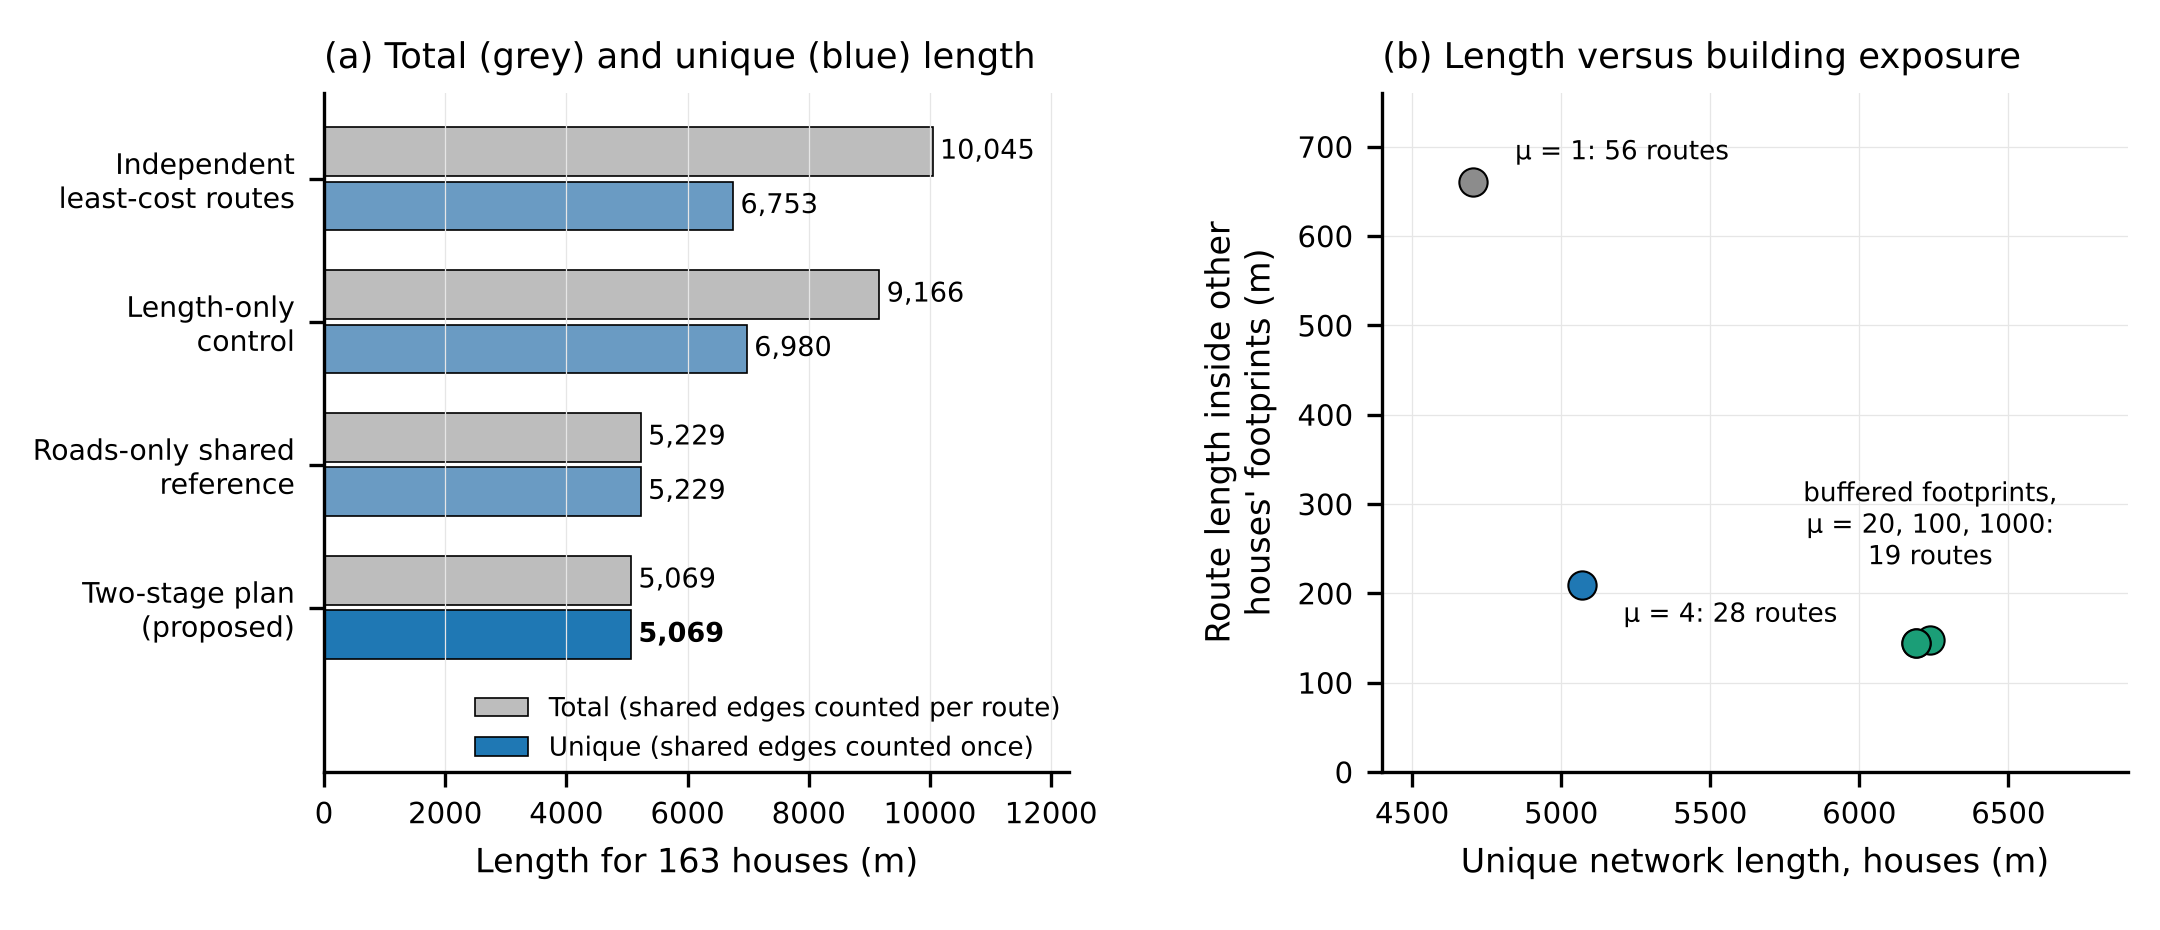
\includegraphics[width=\textwidth]{figures/fig3_routing.png}
\caption{Damarakunta routing results for 163 houses. (a)~Total and unique corridor length by strategy. (b)~Unique network length against route length inside other houses' footprints for $\mu=1$, $\mu=4$ and buffered footprints with large penalties.}
\label{fig:routing}
\end{figure}

\subsection{Impact of building omissions}
Table~\ref{tab:omission} and figure~\ref{fig:omission} summarise the omission analysis against the 5{,}069~m baseline. Missing buildings make the plan \emph{shorter}: 10\% random omission (16 houses) understates length by 7.6\%, 20\% by 16.9\%, omission of the smallest quarter by 25.1\% and omission of all merged blobs by 29.4\%. At the same time $U$ households lose access: 16 and 33 for random 10\% and 20\% omission, 41 for the smallest quarter and 62 (38.0\%) for merged blobs. A planner reading only total length would therefore underfund the scheme. Random additions lengthen the plan by 8.6\% and 15.8\%. The saving $\rho$ stays within 24.9--26.6\% across omissions, so the benefit of sharing is robust to inventory error.

\begin{table}[t]
\caption{Impact of simulated omissions and additions, Damarakunta. Baseline 5{,}069.0~m, 163 routed. Random scenarios are means of five draws. $U$: households without a route; $\kappa$: coverage; $\delta_L$: change in unique length; $\bar\ell$: length per routed target; $\rho$: saving against independent routing.}
\label{tab:omission}
\centering
\small
\begin{tabular}{@{}lrrrrrrr@{}}
\toprule
Scenario & Routed & $U$ & $\kappa$ (\%) & $L$ (m) & $\delta_L$ (\%) & $\bar\ell$ (m) & $\rho$ (\%)\\
\midrule
Baseline & 163 & 0 & 100.0 & 5{,}069.0 & 0.0 & 31.1 & 24.9\\
Omit 10\% (random) & 147.0 & 16 & 90.2 & 4{,}684.4 & $-7.6$ & 31.9 & 25.1\\
Omit 20\% (random) & 130.0 & 33 & 79.8 & 4{,}211.5 & $-16.9$ & 32.4 & 24.9\\
Omit smallest 10\% & 146 & 17 & 89.6 & 4{,}648.6 & $-8.3$ & 31.8 & 24.9\\
Omit smallest 25\% & 122 & 41 & 74.8 & 3{,}798.3 & $-25.1$ & 31.1 & 25.6\\
Omit merged blobs & 101 & 62 & 62.0 & 3{,}579.0 & $-29.4$ & 35.4 & 26.6\\
\midrule
Add 10\% (random) & 177.4 & --- & --- & 5{,}502.4 & $+8.6$ & 31.0 & 25.6\\
Add 20\% (random) & 190.6 & --- & --- & 5{,}868.3 & $+15.8$ & 30.8 & 25.4\\
\bottomrule
\end{tabular}
\end{table}

\begin{figure}[t]
\centering
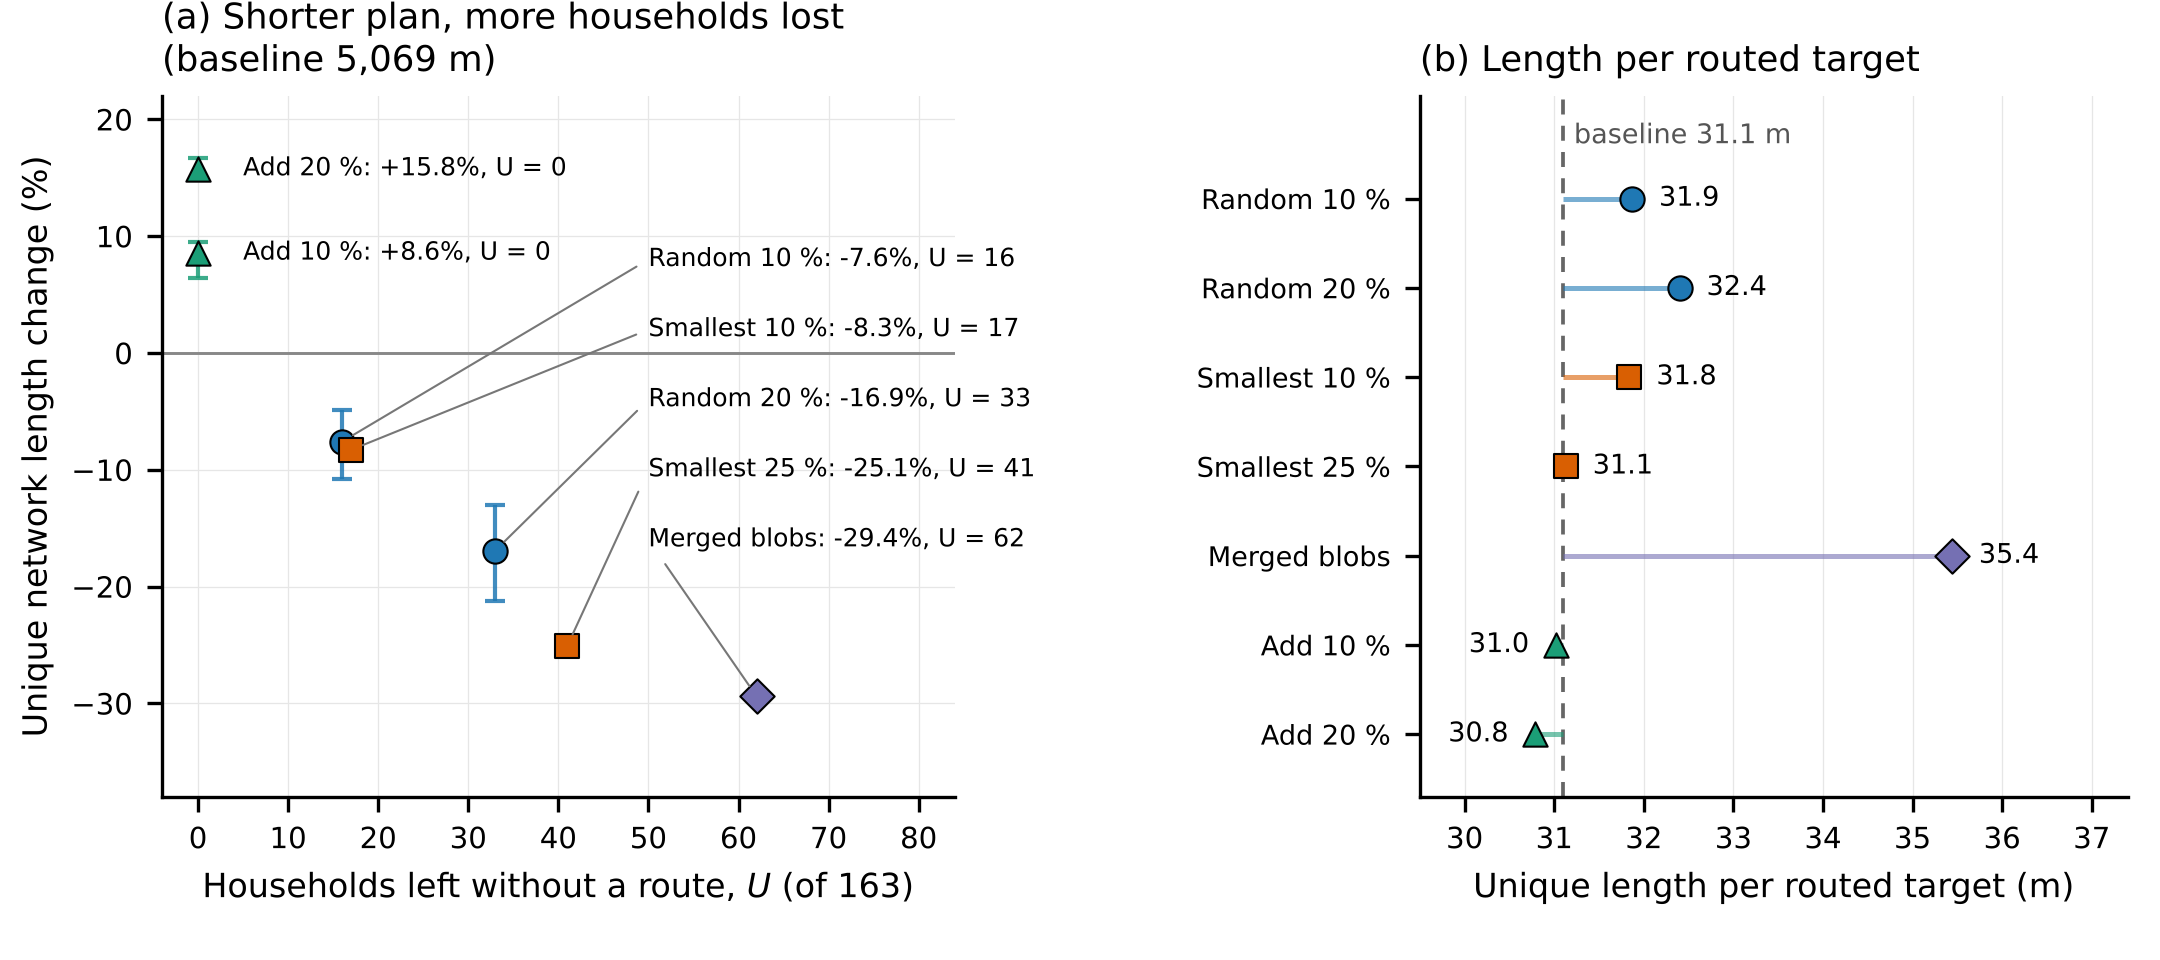
\includegraphics[width=\textwidth]{figures/fig4_omission.png}
\caption{Damarakunta omission sensitivity (163 baseline targets, 5{,}069~m; random scenarios are five draws with min--max bars). (a)~Change in unique length against households left without a route. (b)~Unique length per routed target.}
\label{fig:omission}
\end{figure}

\section{Results: transfer to Adilabad Urban}\label{sec:adilabad}
\subsection{Road-gap targets and routing}
\emph{End-to-end run (\dinoseg{} footprints).} Of the 2{,}690 footprints of at least 30~m$^2$, 345 lie more than 30~m from a road and form the targets (Damarakunta: 163). The planner routes all 345. Independent least-cost routes total 23{,}312.5~m (unique 21{,}440.8~m); the two-stage plan needs 18{,}288.7~m, a saving of 14.7\% (table~\ref{tab:adilabad}; the routes are drawn in figure~\ref{fig:flow}). The roads-only shared reference saves 2.3\% and the length-only control 6.9\%, so almost all of the saving comes from sharing among new routes. Exposure: 54 of 345 routes (15.7\%) cross another footprint (398.0~m), against 28 of 163 (17\%) in Damarakunta.

These numbers must be read with the extraction quality in mind. More than half of the instances (1{,}580 of 2{,}769) are \textsc{Unresolved\_Merge} blobs with a median area of 1{,}125.5~m$^2$: in the dense fabric the segmenter merges neighbouring roofs, so the 345 targets are built-up units rather than houses, and the footprint penalty acts on merged blocks. No reference mask exists for Adilabad, so detection accuracy there is not known.

\emph{Open-footprint check.} With 874 road-gap targets (873 routed) among 18{,}242 Overture footprints (median footprint 139.6~m$^2$, median distance to the nearest road 42.3~m), independent routes total 56{,}308.0~m (unique 46{,}419.2~m) and the two-stage plan 34{,}358.8~m, a saving of 26.0\%; the roads-only reference saves 2.9\% and the length-only control 5.7\%; 332 of 873 routes (38\%) cross another footprint (2{,}041.1~m). The facility phase connects 71 verified facilities with 1{,}090.1~m of unique corridor.

Both Adilabad variants agree that sharing helps (14.7\% and 26.0\%) and that a roads-only reference does not (2.3\% and 2.9\%, against 22.6\% in Damarakunta), but they differ in the size of the saving. This is consistent with fewer, more widely spaced targets (345 against 874) offering less opportunity to share, an explanation that was not tested. The comparison is between two footprint sources, not a validation of either.

\begin{table}[t]
\caption{Cross-settlement comparison under the same cost surface and solver. ``Seg.'' = \dinoseg{} footprints on Esri imagery; ``open'' = Overture footprints. Targets are defined by different rules (all candidates in Damarakunta, road-gap houses in Adilabad).}
\label{tab:adilabad}
\centering
\footnotesize
\begin{tabular}{@{}>{\raggedright\arraybackslash}p{5.6cm}rrr@{}}
\toprule
Metric & Damarakunta & Adilabad seg. & Adilabad open\\
\midrule
Study area (km$^2$) & 18.47 & 17.75 & 17.75\\
Targets / routed & 163 / 163 & 345 / 345 & 874 / 873\\
Independent routes, unique (m) & 6{,}753.1 & 21{,}440.8 & 46{,}419.2\\
Length-only control, unique (m) & 6{,}979.8 & 19{,}961.2 & 43{,}787.2\\
Roads-only shared reference, unique (m) & 5{,}229.3 & 20{,}947.0 & 45{,}058.9\\
\textbf{Two-stage plan, unique (m)} & \textbf{5{,}069.0} & \textbf{18{,}288.7} & \textbf{34{,}358.8}\\
Saving vs.\ independent (\%) & 24.9 & 14.7 & 26.0\\
Roads-only shared saving (\%) & 22.6 & 2.3 & 2.9\\
Unique length per routed house (m) & 31.1 & 53.0 & 39.4\\
Routes crossing other footprints & 28 of 163 & 54 of 345 & 332 of 873\\
Length inside other footprints (m) & 209.1 & 398.0 & 2{,}041.1\\
$\mu=1\rightarrow4$: unique length change (\%) & $+7.7$ & $+9.2$ & $+13.3$\\
$\mu=1\rightarrow4$: routes crossing & 56 $\rightarrow$ 28 & 138 $\rightarrow$ 54 & 618 $\rightarrow$ 332\\
10\% random omission: change (\%) / unserved & $-7.6$ / 16 & $-8.8$ / 34 & $-7.6$ / 88\\
20\% random omission: change (\%) / unserved & $-16.9$ / 33 & $-18.3$ / 69 & $-15.0$ / 176\\
Smallest-25\% omission: change (\%) / unserved & $-25.1$ / 41 & $-21.2$ / 87 & $-21.2$ / 220\\
\bottomrule
\end{tabular}
\end{table}
\subsection{Robustness}
\emph{Footprint penalty.} Raising $\mu$ from 1 to 4 lengthens the unique network by 9.2\% and removes 84 crossing routes (138 to 54); $\mu=20$ and 100 give 19{,}777.0~m and 19{,}924.5~m with 49 and 48 routes crossing, and buffered footprints give 22{,}757.0~m and 23{,}475.5~m with 7 crossing each (table~\ref{tab:sens}, figure~\ref{fig:adilsens}a). The saving against independent routing stays between 10.1\% and 17.7\% across all settings (open footprints: 17.8\% to 30.8\%, table~\ref{tab:sens_open}).

\emph{Road-gap threshold.} Targets defined as houses more than 20, 30 or 50~m from a road number 750, 345 and 129 and give savings of 10.6\%, 14.7\% and 18.5\% (open footprints: 2{,}190, 874 and 296 targets; 21.9\%, 26.0\% and 29.5\%). The saving therefore depends on the target definition, which should be reported with any such result.

\emph{Omissions.} Random omission of 10\% and 20\% (five seeds) changes unique length by $-8.8\%$ (range $-11.7$ to $-6.5$) and $-18.3\%$ ($-21.9$ to $-15.8$), leaving 34 and 69 targets unserved; single-run smallest-10\% and smallest-25\% omissions give $-8.0\%$ and $-21.2\%$ (35 and 87 unserved). As in Damarakunta and in the open-footprint check, missing buildings shorten the plan while stranding households, and the saving stays at 12.6--14.1\%. With open footprints the same scenarios give $-7.6\%$, $-15.0\%$, $-7.9\%$ and $-21.2\%$ and a saving of 23.8--25.2\%. Merged-blob and addition scenarios were not defined for Adilabad.

\begin{table}[t]
\caption{Adilabad sensitivity, \dinoseg{} footprints (345 targets unless stated). Top: footprint-penalty settings. Bottom: road-gap threshold.}
\label{tab:sens}
\centering
\footnotesize
\begin{tabular}{@{}lrrrrr@{}}
\toprule
Setting & Unique (m) & $\rho$ (\%) & Crossing routes & In footprints (m) & Targets\\
\midrule
Centre-in-footprint, $\mu=1$ & 16{,}740.5 & 17.7 & 138 & 1{,}479.8 & 345\\
Centre-in-footprint, $\mu=4$ & 18{,}288.7 & 14.7 & 54 & 398.0 & 345\\
Centre-in-footprint, $\mu=20$ & 19{,}777.0 & 12.5 & 49 & 356.4 & 345\\
Centre-in-footprint, $\mu=100$ & 19{,}924.5 & 12.2 & 48 & 343.2 & 345\\
Buffered 7.1~m, $\mu=20$ & 22{,}757.0 & 10.1 & 7 & 57.9 & 345\\
Buffered 7.1~m, $\mu=100$ & 23{,}475.5 & 10.6 & 7 & 55.7 & 345\\
\midrule
Gap $>20$~m & 30{,}621.7 & 10.6 & 69 & 442.8 & 750\\
Gap $>30$~m (primary) & 18{,}288.7 & 14.7 & 54 & 398.0 & 345\\
Gap $>50$~m & 9{,}155.2 & 18.5 & 28 & 251.9 & 129\\
\bottomrule
\end{tabular}
\end{table}

\begin{table}[t]
\caption{Adilabad sensitivity, open Overture footprints (874 targets, 873 routed). Top: footprint-penalty settings. Bottom: road-gap threshold.}
\label{tab:sens_open}
\centering
\footnotesize
\begin{tabular}{@{}lrrrrr@{}}
\toprule
Setting & Unique (m) & $\rho$ (\%) & Crossing routes & In footprints (m) & Targets\\
\midrule
Centre-in-footprint, $\mu=1$ & 30{,}335.7 & 30.8 & 618 & 4{,}893.0 & 874\\
Centre-in-footprint, $\mu=4$ & 34{,}358.8 & 26.0 & 332 & 2{,}041.1 & 874\\
Centre-in-footprint, $\mu=20$ & 37{,}024.1 & 22.8 & 271 & 1{,}687.4 & 874\\
Centre-in-footprint, $\mu=100$ & 37{,}513.9 & 21.7 & 275 & 1{,}744.8 & 874\\
Buffered 7.1~m, $\mu=20$ & 42{,}071.9 & 20.1 & 231 & 1{,}397.2 & 874\\
Buffered 7.1~m, $\mu=100$ & 44{,}094.6 & 17.8 & 221 & 1{,}310.5 & 874\\
\midrule
Gap $>20$~m & 65{,}204.4 & 21.9 & 815 & 4{,}543.9 & 2{,}190\\
Gap $>30$~m (primary) & 34{,}358.8 & 26.0 & 332 & 2{,}041.1 & 874\\
Gap $>50$~m & 15{,}880.9 & 29.5 & 126 & 809.9 & 296\\
\bottomrule
\end{tabular}
\end{table}

\begin{figure}[t]
\centering
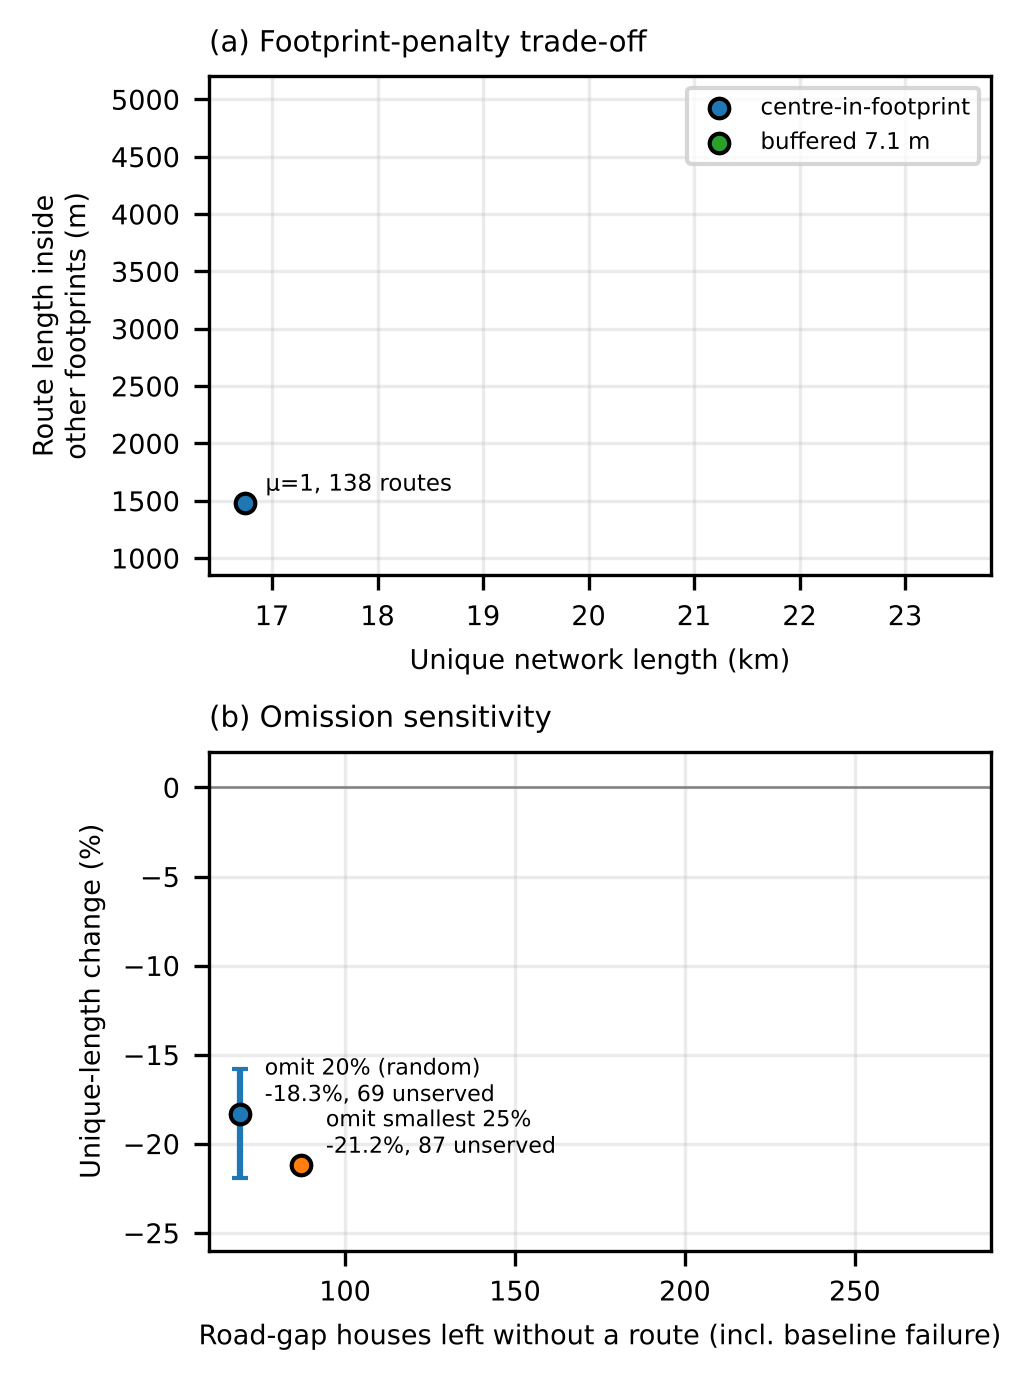
\includegraphics[width=0.5\textwidth]{figures/adilabad_seg_sens_col.png}
\caption{Adilabad sensitivity (\dinoseg{} footprints). (a)~Footprint-penalty trade-off between unique network length and route length inside other footprints. (b)~Omission sensitivity (random: mean and min--max over five seeds; smallest-$q$: single run).}
\label{fig:adilsens}
\end{figure}

\section{Results: four study areas with zero-crossing clearance}\label{sec:four}
Figure~\ref{fig:flow} follows the chain of figure~\ref{fig:arch} for the four study areas, from the Telangana locator through the input imagery and roads, the extracted footprints and verified facilities, to the planned network. Table~\ref{tab:four} collects every metric of the four areas in one place; it is regenerated by \texttt{scripts/run\_village\_pipeline.py --compare-all}, and a red \pending{value} marks a number not yet computed on the machine that wrote the table. The Adilabad column uses the updated settlement boundary (a derived built-up extent of Adilabad town) and the segmentation footprints of that boundary, so it is not the 2018 mandal experiment of the preceding sections.

On the 5~m clearance grid, Stage~B shortens the unique network relative to the independent Stage~A routes by Damarakunta 21.0\%, Adilabad 12.2\%, Aswaraopeta 25.3\%, Alampur 16.2\%. Building crossings are zero in every area by construction and were verified by intersecting every drawn route with all footprints, whereas the ten-metre soft-penalty plan ($\mu=4$) still leaves routes across other footprints (Damarakunta 28, Adilabad 99, Aswaraopeta 157, Alampur 5 routes, respectively). Targets with no free lane to the road network are reported as unrouted rather than routed over a roof, so the routed counts in table~\ref{tab:four} are below the target counts where buildings enclose a house. The segmentation rows are model-level: they are the LoveDA validation scores of the one checkpoint used for all four areas, not accuracy on any of the four areas, for which no surveyed reference exists. Costs use the owner-supplied, unverified PMGSY-based rate of Rs 75 lakh/km and are illustrative.

\begin{figure*}[p]
\centering
\IfFileExists{figures/fig_flow_study_areas.png}{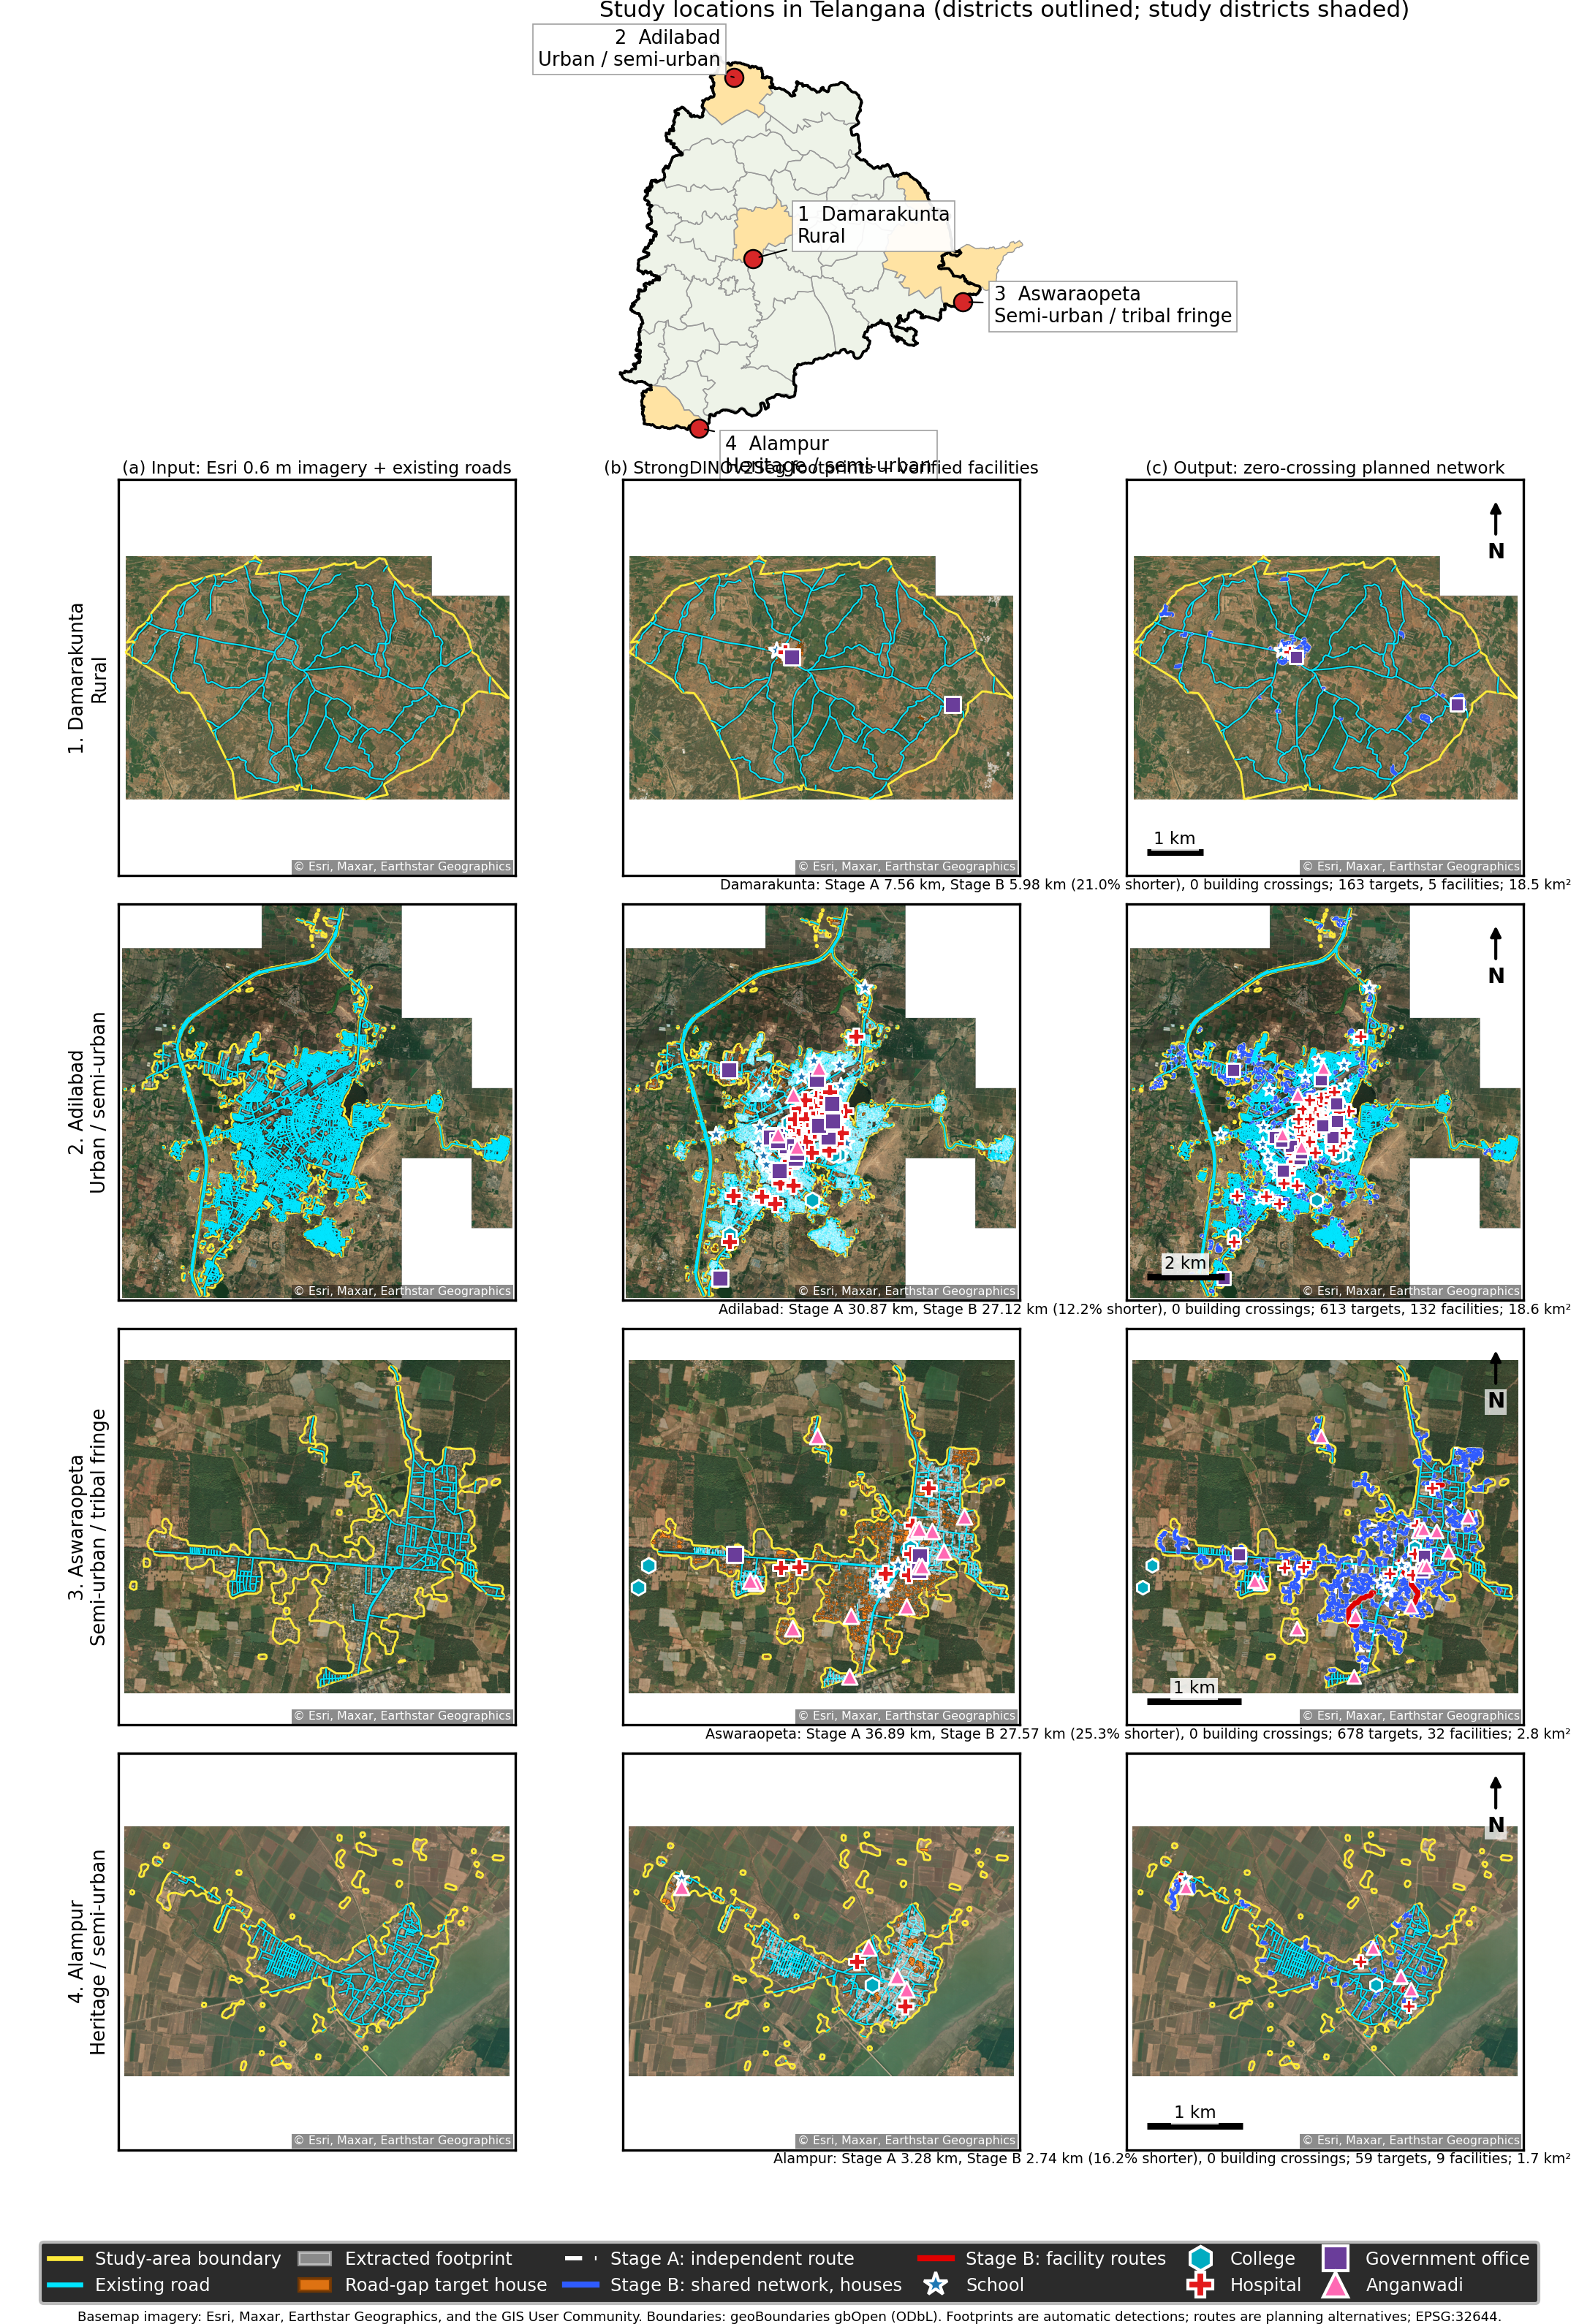
\includegraphics[width=0.93\textwidth]{figures/fig_flow_study_areas.png}}{\fbox{\parbox{0.8\textwidth}{\centering\pending{Figure not generated yet: run \texttt{python scripts/build\_paper\_flow\_figure.py --source segmentation} on the PC that holds the segmentation results.}}}}
\caption{Study areas and end-to-end flow. Top: Telangana with district outlines and the four study locations (1~Damarakunta, rural; 2~Adilabad, urban / semi-urban; 3~Aswaraopeta, semi-urban / tribal fringe; 4~Alampur, heritage / semi-urban). Rows 1--4: (a)~input, Esri World Imagery (0.6~m) with the existing road network; (b)~\dinoseg{} footprints (road-gap target houses in orange) with the verified facilities (School, College, Hospital, Government Office, Anganwadi); (c)~output, existing roads, Stage~A independent routes (white dashed) and Stage~B shared network (blue: houses; red: facilities) with the 5~m zero-crossing clearance, scale bar and north arrow. Basemap imagery: Esri, Maxar, Earthstar Geographics, and the GIS User Community. Footprints are automatic detections and routes are planning alternatives, not engineered roads.}
\label{fig:flow}
\end{figure*}

\begin{table*}[t]
\caption{Four study areas side by side. Segmentation rows: LoveDA validation of the single \dinoseg{} checkpoint (macro averages; F1-score equals the mean Dice). Routing rows: unique lengths on the 5~m zero-crossing grid (Stage~A independent, Stage~B shared network, shared edges once); building crossings are routes inside another building's footprint; the cost is the Stage~B length times Rs 75 lakh per km (range 60--90), an owner-supplied, unverified PMGSY-based rate, so it is illustrative and not an engineering estimate.}
\label{tab:four}
\centering
\scriptsize
\resizebox{\textwidth}{!}{% generated by scripts/run_village_pipeline.py --compare-all (do not edit by hand); \pending{...} marks a value not yet computed on the machine that generated this file
\begin{tabular}{@{}lrrrr@{}}
\toprule
Metric & Damarakunta & Adilabad & Aswaraopeta & Alampur \\
\midrule
\multicolumn{5}{@{}l}{\textit{Study area profile}}\\
District & Siddipet & Adilabad & Bhadradri Kothagudem & Jogulamba Gadwal \\
Typology & Rural & Urban / semi-urban & Semi-urban / tribal fringe & Heritage / semi-urban \\
Window area (km$^2$) & 18.47 & 18.59 & 2.82 & 1.65 \\
Existing road length (km) & 51.7 & 509.9 & 28.6 & 25.3 \\
\midrule
\multicolumn{5}{@{}l}{\textit{Segmentation and extraction (model metrics: LoveDA validation, one checkpoint for all areas)}}\\
Overall accuracy (\%) & \multicolumn{4}{c}{71.3} \\
Precision, macro (\%) & \multicolumn{4}{c}{72.4} \\
Recall, macro (\%) & \multicolumn{4}{c}{66.9} \\
F1-score = mean Dice (\%) & \multicolumn{4}{c}{68.9} \\
mIoU (\%) & \multicolumn{4}{c}{53.8} \\
Extracted building footprints & 165 & 5{,}653 & 1{,}297 & 430 \\
\midrule
\multicolumn{5}{@{}l}{\textit{Verified public infrastructure (audited, on building footprints)}}\\
School & 2 & 39 & 5 & 1 \\
College & 0 & 15 & 3 & 1 \\
Hospital & 1 & 59 & 7 & 2 \\
Government office & 2 & 15 & 3 & 0 \\
Anganwadi & 0 & 4 & 14 & 5 \\
Total verified facilities & 5 & 132 & 32 & 9 \\
\midrule
\multicolumn{5}{@{}l}{\textit{Stage A vs.\ Stage B routing (5\,m zero-crossing clearance) and PMGSY-benchmarked cost}}\\
Road-gap target buildings & 163 & 613 & 678 & 59 \\
Routed buildings & 162 & 607 & 632 & 58 \\
Stage A independent length (km) & 7.56 & 30.87 & 36.89 & 3.28 \\
Stage B shared-trunk length (km) & 5.98 & 27.12 & 27.57 & 2.74 \\
Corridor length saving (\%) & 21.0 & 12.2 & 25.3 & 16.2 \\
Building crossings (routes) & 0 & 0 & 0 & 0 \\
Mean terrain slope (\%) & 3.8 & 3.1 & 3.1 & 2.1 \\
PMGSY-benchmarked cost (INR lakh) & 448 & 2{,}034 & 2{,}067 & 206 \\
\bottomrule
\end{tabular}
% PMGSY-benchmarked cost = unique Stage B length (km) x Rs 75 lakh/km (sensitivity range 60-90)
}
\end{table*}

\section{Discussion}
\subsection{What transfers and what does not}
The planning stages transferred without modification: the same cost surface, solver parameters and metrics produced connected plans in a dense window, both from \dinoseg{} footprints on Esri imagery (345 targets) and from open footprints (874 targets). The qualitative findings were reproduced in all three settings: sharing saves unique length (24.9\%, 14.7\% and 26.0\%), the footprint penalty trades length for exposure, and omissions shorten the plan while stranding households. What did not transfer is the benefit of the simpler baselines: roads-only sharing recovered most of the gain in the dispersed village (22.6\%) but almost none in the dense window (2.3\% and 2.9\%), which suggests that the value of a marginal-cost planner grows with settlement density, a hypothesis supported by one dense window. The two Adilabad footprint sources differ in the size of the saving (14.7\% against 26.0\%); with 57\% of the segmented instances being merged blocks, the segmentation result may reflect coarse, widely spaced targets, and no reference mask exists to say which footprint set is closer to the truth.

\subsection{Why pixel metrics are not enough for infrastructure use}
Segmentation metrics are area-weighted over classes, while the planner counts instances. A detector that misses the smallest quarter of buildings can lose few building pixels yet removes a quarter of households from the plan (table~\ref{tab:omission}), and a detector that merges adjacent roofs can score a high pixel IoU yet strands 38\% of the Damarakunta houses in the merged-blob scenario. Network length falls in both cases, so total length is a poor quality indicator. Merged blobs correspond to dense multi-roof structures; whether they coincide with the core of a hamlet was not measured.

\subsection{Land take and planning use}
Shared corridors reduce the length of new road for the same households. As an illustration only, assuming a 5~m formation width (an assumption of this study; no road-width data were available), the 1{,}684~m saved in Damarakunta corresponds to about 0.84~ha less land take, the 3{,}152~m saved in Adilabad (segmentation targets) to about 1.6~ha and the 12{,}060~m saved against the open-footprint targets to about 6.0~ha. For PMGSY-style schemes \cite{pmgsy} three points follow. Building inventories are uncertain inputs and a network sized from them should carry a sensitivity band. Shared corridors save about a quarter of unique length and this survives omissions. Local overrides should be used sparingly and documented. The outputs are screening-level alternatives; we do not claim compliance with Indian Roads Congress design standards, nor any engineering design value.

\subsection{Limitations}
(i) Two settlements only; the semi-urban and second rural windows are planned but have not been run. (ii) Omission scenarios are synthetic, not measured detection errors. (iii) Neither Damarakunta nor Adilabad has a surveyed reference mask; the LoveDA metrics come from the epoch-4 checkpoint with metadata recovered from the training notebook, and the checkpoint hash (SHA-256 \texttt{2e7c4646dc77ceb2\allowbreak a357f44f11cb3f7f\allowbreak f84e636871d70ba4\allowbreak c31e194e5ec00cf3}) was logged only for the Adilabad run, not with the Damarakunta candidates, although both runs loaded the same file path. (iv) In Adilabad 57\% of the \dinoseg{} instances are \textsc{Unresolved\_Merge} blocks, so its 345 targets are built-up units, not houses; the open footprints are map data of unverified completeness, and Overture licences were not re-verified. Ten of the 68 verified facility points share an identical coordinate with another Overture record (generic geocodes), so the 20 m footprint check is weak evidence in the dense fabric. (v) Costs are ordinal, the planner is a heuristic without an optimality guarantee, and road-gap targeting changes the problem, as the threshold sweep shows. (vi) Pixel accuracy is reported as 71.3\%, the value recomputed from the confusion matrix. (vii) Merged-blob and addition scenarios were run only for Damarakunta.

\section{Conclusions}
A pipeline from satellite imagery and open layers to shared access roads connects the houses and facilities of a rural village (24.9\% less unique corridor than independent routing) and, without changes to the cost surface or solver, those of an urban and peri-urban mandal, end to end on Esri imagery (14.7\% less) and on open footprints (26.0\% less). Footprint penalties and simulated inventory errors behave consistently in all three settings: penalties trade length for fewer routes through dwellings, and omissions shorten the plan while stranding households. The dependence of the roads-only baseline on settlement density, and the effect of detection quality across settings, are the main open questions; a semi-urban and a second rural window are planned to address the first.

\ifanon\else
\section*{Acknowledgments}
The authors acknowledge the Telangana State Remote Sensing Application Centre (TGRAC) for the boundary, road and facility layers of Damarakunta, and the providers of the open datasets used (ESA WorldCover, Copernicus DEM, Overture Maps, geoBoundaries, Google Open Buildings, LoveDA).
\fi

\section*{Data sources and imagery attribution}
High-resolution RGB satellite basemap imagery for Damarakunta Village and the Adilabad Urban window was obtained via Esri World Imagery (sources: Esri, Maxar, Earthstar Geographics, and the GIS User Community) and used strictly for non-commercial academic research and visual overlay in accordance with Esri's academic use terms, while raw imagery tiles are not redistributed. All derived modeling and multi-settlement planning layers rely on open-licensed datasets: ESA WorldCover 10~m v200 (CC BY 4.0), Copernicus GLO-30 DEM (Copernicus Open Access Licence), geoBoundaries ADM3 (ODbL 1.0), and Overture Maps (ODbL 1.0 / CDLA-Permissive-2.0). Damarakunta's boundary, road and facility layers are TGRAC data and its $\sim$30~m DEM source was not recorded; the Copernicus GLO-30 and geoBoundaries layers apply to the Adilabad window.

\section*{Funding}
This research received no specific grant from any funding agency in the public, commercial, or not-for-profit sectors.

\section*{Data availability statement}
\ifanon
Code, derived tables and the open-data manifests (with SHA-256 hashes) will be made available in a public repository on acceptance and are available to reviewers on request. TGRAC layers for Damarakunta are subject to the provider's terms.
\else
Code, derived summary tables, and the open-data manifests with SHA-256 hashes are available at \url{https://github.com/Archana519/Telangana-Rural-Project} (folders \path{DELIVERABLES_DAMARAKUNTA_STAGE_B} and \path{DELIVERABLES_CONTRIBUTION_3_MULTI_VILLAGE}, the latter including the Adilabad segmentation results in \path{01_ADILABAD_SEGMENTATION}). TGRAC layers for Damarakunta are subject to the provider's terms. The \dinoseg{} checkpoint is not included in the repository; its SHA-256 is given in Section~\ref{sec:methods}. A Zenodo DOI will be added when the archive is minted.
\fi

\section*{Conflict of interest}
The authors declare no competing interests.

\bibliographystyle{unsrt}
\bibliography{references}

\end{document}
"      (then bibtex / pdflatex as above)
% The IOP class (iopjournal / iopart) is not installed in this build environment, so the manuscript uses a plain
% `article` layout with the same logical front matter. At submission, paste the sections into the IOP journal
% template (Overleaf: "IOP journal article template", option [anonymous] for double-anonymous review).
% Every number in Sections 3-5 is checked by paper_eris/verify_eris_numbers.py against
% DELIVERABLES_DAMARAKUNTA_STAGE_B/ and DELIVERABLES_CONTRIBUTION_3_MULTI_VILLAGE/01_ADILABAD/.
% =============================================================================================================
\documentclass[12pt,a4paper]{article}
\usepackage[margin=2.5cm]{geometry}
\usepackage{setspace}\onehalfspacing
\usepackage{graphicx}
\usepackage{booktabs}
\usepackage{array}
\usepackage{amsmath,amssymb}
\usepackage{url}
\usepackage{xcolor}
\usepackage{algorithm}
\usepackage{algpseudocode}
\usepackage[hidelinks]{hyperref}
\setlength{\emergencystretch}{3em}
\newif\ifanon
\ifdefined\ANON\anontrue\fi
\newcommand{\dinoseg}{StrongDINOv2Seg}
\newcommand{\Lcost}{L_{\mathrm{cost}}}
\newcommand{\pending}[1]{\textcolor{red}{\textit{#1}}}% value not yet computed on the machine that generated paper_comparison_table.tex
\algrenewcommand\algorithmicrequire{\textbf{Input:}}
\algrenewcommand\algorithmicensure{\textbf{Output:}}

\begin{document}

\begin{center}
{\Large\bfseries Smart village infrastructure planning and road network optimization for rural Telangana\par}
\vspace{0.8em}
\ifanon
{\large [Authors withheld for double-anonymous review]\par}
\else
\small\begin{tabular}{@{}p{0.47\textwidth}p{0.47\textwidth}@{}}
\centering\textbf{Ramakrishna Kolikipogu}\par
\centering\textit{Department of Information Technology}\par
\centering\textit{Chaitanya Bharathi Institute of Technology (A)}\par
\centering Hyderabad, India\par
\centering krkrishna.cse@gmail.com\par
&
\centering\textbf{Pendyala Archana}\par
\centering\textit{Department of Information Technology}\par
\centering\textit{Chaitanya Bharathi Institute of Technology (A)}\par
\centering Hyderabad, India\par
\centering pendyalaarchanareddy98@gmail.com\par
\end{tabular}\\[1.4em]
\fi
\end{center}

\begin{abstract}
\noindent Rural road infrastructure planning faces several challenges, including incomplete spatial data, unplanned settlements, difficult terrain, and limited information about suitable road connections to essential public services such as hospitals, schools, and government institutions. Conventional road-planning approaches often rely on manual decision-making and shortest-path algorithms, which may not adequately consider the influence of spatial-data errors, terrain conditions, land-use constraints, and opportunities for sharing road segments. To address these challenges, this work proposes an AI- and GIS-based framework for rural village infrastructure planning and road-network optimization. The proposed framework integrates high-resolution satellite imagery, existing road-network data, village boundary information, land-cover maps, elevation data, and public-service locations. A StrongDINOv2Seg deep-learning model is employed for semantic segmentation, supported by GIS-based feature extraction to identify relevant spatial features. A multi-criteria cost surface is then generated by considering land-cover conditions, terrain slope, and restricted areas to identify suitable movement paths. For road-network planning, a two-stage approach is implemented: in the first stage, alternative least-cost routes are generated using grid-based Dijkstra pathfinding; in the second stage, a greedy shared-network selection strategy evaluates alternative routes based on their marginal cost and gives credit to road segments already included in the selected network, reducing unnecessary route duplication while prioritizing connections to public-service facilities and residential buildings. The framework is demonstrated on Damarakunta village in Siddipet District, Telangana, and evaluated for cross-morphology transferability in Adilabad Urban. On the LoveDA validation benchmark, the segmentation model achieved a mean Intersection over Union (mIoU) of 53.8\% and a mean Dice score of 68.9\%. In the Damarakunta building-access planning experiment, the two-stage network-aware approach produced 5{,}069.0~m of unique route length compared with 6{,}753.1~m for independent least-cost routing, representing a reduction of 24.9\%. Re-applied end to end to Adilabad Urban on Esri imagery, the same cost surface and solver reduced unique route length from 21{,}440.8~m to 18{,}288.7~m (14.7\%) for 345 road-gap targets, and with open Overture Maps footprints from 46{,}419.2~m to 34{,}358.8~m (26.0\%), confirming consistent network-sharing behavior across contrasting settlement densities, although a roads-only shared reference recovered most of the saving in Damarakunta (22.6\%) but little in Adilabad (2.3\% and 2.9\%). Because most StrongDINOv2Seg instances in Adilabad's dense fabric are merged roof blocks, its targets are built-up units rather than counted houses. The proposed framework provides a GIS-based decision-support approach for analyzing rural infrastructure requirements and generating cost-aware road-network alternatives as computational planning suggestions requiring field validation prior to implementation.
\end{abstract}

\noindent\textit{Keywords}: rural roads, building footprint extraction, satellite remote sensing, least-cost path, shared network, spatial transferability, open geospatial data, Telangana

\section{Introduction}
Road building is among the most consequential land-use changes of the coming decades. Global road length is projected to grow by roughly 3.0--4.7 million km by 2050 \cite{meijer2018global}, and new roads open land to clearing, fragmentation and conversion \cite{laurance2014global}. Much of this growth is local. In India the Pradhan Mantri Gram Sadak Yojana (PMGSY) connects habitations through all-weather rural roads \cite{pmgsy}, and planning for such schemes depends on knowing where dwellings and facilities are, what terrain and land cover a corridor must cross, and which connection rule is applied.

Computational support for this planning has matured along three separate lines. Remote sensing now maps buildings and roads at large scale, from continental building inventories \cite{sirko2021openbuildings} to foundation-model segmenters \cite{oquab2023dinov2}, with recent work addressing small and isolated rural buildings, uncertainty, and domain shift \cite{r62,r63,r64,r65,r66,r67,r68,r69,r70}. Multi-criteria and least-cost analysis translates terrain and land cover into route costs \cite{r06,r53,r54,collischonn2000lcp}. Network-design formulations connect many demand points at low total cost, including Steiner-tree heuristics \cite{kou1981steiner,mehlhorn1988steiner,hwang1992steiner,r51}, rural road design models \cite{r41,r43,r44} and recent analogues for power and transport networks \cite{r45,r46,r47,r50}. These lines are rarely joined: detectors are judged by pixel overlap \cite{r01}, planners assume an error-free inventory, and each house is often connected independently, so neighbouring houses re-trace the same corridor.

We join them in a single reproducible pipeline and test it at two settlement densities. Our contributions are:
\begin{enumerate}
\item \textbf{End-to-end pipeline.} A pipeline from satellite imagery to a shared access network: StrongDINOv2Seg segmentation, OpenCV/NumPy distance-transform instance extraction with an explicit merge flag, a multi-criteria cost surface with a footprint penalty, and a two-stage shared-network planner (Section~\ref{sec:methods}).
\item \textbf{Error propagation.} Controlled omission and addition scenarios that propagate building-inventory errors through the planner, measuring their effect on unique length, coverage and exposure of dwellings (Sections~\ref{sec:damar}--\ref{sec:adilabad}).
\item \textbf{Multi-settlement spatial transferability and open-data scalability.} The rural Damarakunta workflow is re-applied, with the same cost-surface definition and solver, to the Adilabad Urban mandal (urban and peri-urban): end to end on Esri imagery (StrongDINOv2Seg and instance extraction) and, as an independent check, on open Overture Maps footprints, with a road-gap rule for targets and robustness examined over penalty settings, road-gap thresholds and synthetic omissions (Section~\ref{sec:adilabad}).
\end{enumerate}
Two scope limits apply. Only these two settlements were evaluated; a semi-urban and a second rural window are planned but not yet run, so we make no claim about a full rural--semi-urban--urban gradient. And the Adilabad segmentation results are unvalidated: no reference building mask exists, and in the dense fabric most detected instances are merged roof blocks (Section~\ref{sec:adilabad}), so the Adilabad targets are built-up units rather than counted houses.

\section{Related work}
\textbf{Building extraction.} Reviews of building extraction from remote sensing \cite{r01} document the shift from fully convolutional networks \cite{ji2019whu} to transformer and foundation-model encoders. Recent studies target isolated small buildings \cite{r63}, weak supervision \cite{r62}, uncertainty-guided refinement \cite{r64,r65}, and domain generalisation or adaptation across imagery sources \cite{r02,r66,r67,r68,r69,r70}. Road extraction has followed the same path, with width-adaptive, topology-preserving and foundation-model-based networks for rural and arid scenes \cite{r56,r57,r58,r59,r60}, and topological analysis has been used to detect informal settlements worldwide \cite{r48}. Evaluation is overwhelmingly through overlap scores on benchmark data \cite{foody2002status}; the effect of detection errors on downstream infrastructure decisions is rarely quantified, although error propagation in GIS models is long established \cite{heuvelink1998error}.

\textbf{Route and network planning.} Multi-criteria GIS analysis \cite{r06} and least-cost path methods \cite{collischonn2000lcp,r53,r54} underlie corridor selection for roads, with dedicated treatments of slope \cite{r54}, route alternatives \cite{r53} and travel-time uncertainty \cite{r61}, and GIS route reconstruction has been applied to historical transport routes \cite{r55}. Rural road design has been addressed with improved network-design models \cite{r41}, algorithmic planning under constrained capacities in India \cite{r43} and facility-based methodology \cite{r44}. Steiner-tree formulations \cite{hwang1992steiner} and their shortest-path-based heuristics \cite{kou1981steiner,mehlhorn1988steiner} connect many terminals at low total length and are applied to sub-network identification \cite{r51}, multi-terminal routing \cite{r52}, cable routing \cite{r45}, minimum spanning trees of road networks \cite{r46}, rural grids \cite{r47} and least-cost electrification \cite{r50}.

\textbf{Gap.} To our knowledge no cited work combines (i) satellite-derived building instances, (ii) a land-cover- and slope-based cost surface with building avoidance, (iii) a shared-network planner whose marginal cost credits built corridors, and (iv) a systematic test of how inventory omissions and the settlement setting change the result. This paper addresses that combination for rural Telangana and treats the comparison between two settlements as an explicit transferability test.

\section{Study areas and data}
\subsection{Damarakunta (rural)}
Damarakunta is a rural revenue village in Markook mandal, Siddipet district, Telangana ($\approx 17.707^{\circ}$N, $78.753^{\circ}$E). Its boundary, from the Telangana State Remote Sensing Application Centre (TGRAC), encloses 18.47~km$^2$ (UTM zone 44N, EPSG:32644; figure~\ref{fig:flow}). Settlement is dispersed, with small house clusters separated by farmland. A 0.6~m, three-band mosaic (11{,}296 $\times$ 7{,}171 px) was assembled from Esri World Imagery exports. Building candidates are model outputs: 278 polygons, 165 inside the boundary, of which 163 are used as routing targets. They carry a quality class: \textsc{Plausible} (71), \textsc{Review} (32) and \textsc{Unresolved\_Merge} (62), the last denoting blobs that merge adjacent roofs and could not be split. Five TGRAC facilities (schools, a health sub-centre and the gram-panchayat headquarters points) are planned in a separate phase. No ground-truth building mask exists for Damarakunta.

\subsection{Adilabad Urban (urban and peri-urban)}\label{sec:adilabad_data}
The second window is the Adilabad Urban mandal, Adilabad district (geoBoundaries ADM3 polygon; centroid $19.682^{\circ}$N, $78.528^{\circ}$E), 17.75~km$^2$, close to Damarakunta in area. The 10~m grid has 424 $\times$ 564 cells, 177{,}533 of them inside the polygon, 0.62\% blocked (water or slope $>25^{\circ}$). About 60\% of cells are not WorldCover built-up, so the window holds an urban core and a peri-urban fringe. The boundary layer is the 2018 release and may differ from current municipal limits.

Two sets of building footprints are used. (i)~\emph{Segmentation footprints (primary, end to end).} A 0.6~m Esri World Imagery mosaic of the window (7{,}248 $\times$ 9{,}590~px, EPSG:32644) was exported with the Damarakunta recipe (1{,}800~m tiles). \dinoseg{} was applied to 391 tiles of $560\times560$~px (stride 420~px, margin 70~px, the Damarakunta tiling; Damarakunta: 459 tiles) and the same instance extraction. This yields 2{,}769 instances, of which 2{,}690 have an area of at least 30~m$^2$ and form the penalty layer; their quality classes are \textsc{Plausible} (1{,}033), \textsc{Review} (77) and \textsc{Unresolved\_Merge} (1{,}580), the last with a median area of 1{,}125.5~m$^2$ (\textsc{Plausible}: 207.4~m$^2$). Of 83 Overture place candidates inside the window, 68 are verified with the Damarakunta rule (a detected footprint within 20~m): 44 schools, 20 health and 4 government. (ii)~\emph{Open footprints (independent check).} Overture release 2026-10-21.0 \cite{overture2026} supplies 4{,}850 road segments, 24{,}924 building polygons (18{,}846 from OpenStreetMap, 6{,}078 from Google Open Buildings v3 \cite{sirko2021openbuildings}) and 738 places; footprints with area $\ge 30$~m$^2$ and confidence $\ge 0.7$ (18{,}242 polygons) form the penalty layer, and 71 of the 83 facility candidates are verified (44 schools, 20 health, 7 government) after manual removal of mis-geocoded records. Roads are Overture/OSM segments in both variants (table~\ref{tab:data}). Neither footprint set has been field-verified. Figure~\ref{fig:flow} shows the study window, the detected footprints and the verified facilities of every study area.

\begin{table}[t]
\caption{Input data and licence status. ``Not re-verified'' marks Overture licences taken from the provider documentation, which could not be opened from the execution environment.}
\label{tab:data}
\centering
\footnotesize
\begin{tabular}{@{}>{\raggedright\arraybackslash}p{3.0cm}>{\raggedright\arraybackslash}p{5.9cm}>{\raggedright\arraybackslash}p{5.5cm}@{}}
\toprule
Layer & Damarakunta / Adilabad source & Licence status \\
\midrule
Boundary & TGRAC polygon / geoBoundaries ADM3 \cite{runfola2020geoboundaries} & TGRAC: not stated / ODbL 1.0 \\
Roads, facilities & TGRAC (43 road features, 5 facilities) / Overture Maps 2026-10-21.0 \cite{overture2026} & TGRAC: not stated / ODbL 1.0 (roads), CDLA-Permissive-2.0 (places); not re-verified \\
Buildings & StrongDINOv2Seg instances (0.6~m Esri imagery; both windows) / Overture footprints (Adilabad check; OSM, Google Open Buildings v3 \cite{sirko2021openbuildings}) & Esri academic-use terms, tiles not redistributed / ODbL 1.0 and CC BY 4.0; not re-verified \\
Land cover & ESA WorldCover v200, 10~m \cite{zanaga2021worldcover} & CC BY 4.0 \\
Terrain & $\sim$30~m DEM (source not recorded) / Copernicus GLO-30 \cite{esa2022copdem}; Sobel slope, bilinear to 10~m & Not stated / Copernicus Open Access Licence \\
Training benchmark & LoveDA \cite{wang2021loveda} & Source domain only \\
\bottomrule
\end{tabular}
\end{table}

\section{Methods}\label{sec:methods}
The framework is a seven-step chain (figure~\ref{fig:arch}): (1)~multi-source open-data ingestion (Esri World Imagery, ESA WorldCover, Copernicus GLO-30, Overture / OSM / TGRAC roads, the study polygon); (2)~\dinoseg{} semantic segmentation in 560~px tiles; (3)~distance-transform extraction of building footprints and road-gap targets; (4)~a four-pass multi-source facility audit that snaps every facility onto a roof; (5)~a multi-criteria cost surface with a 5~m zero-crossing building clearance; (6)~Stage~A and Stage~B Dijkstra shared-network routing; and (7)~connectivity and PMGSY-based cost evaluation. Steps 1 to 7 are identical for all four study areas; the settlements differ only in their inputs. The ten-metre soft-penalty planner of the earlier experiments is kept as a comparison baseline (section~\ref{sec:damar}), and the clearance network is the proposed plan (section~\ref{sec:four}).

\begin{figure}[t]
\centering
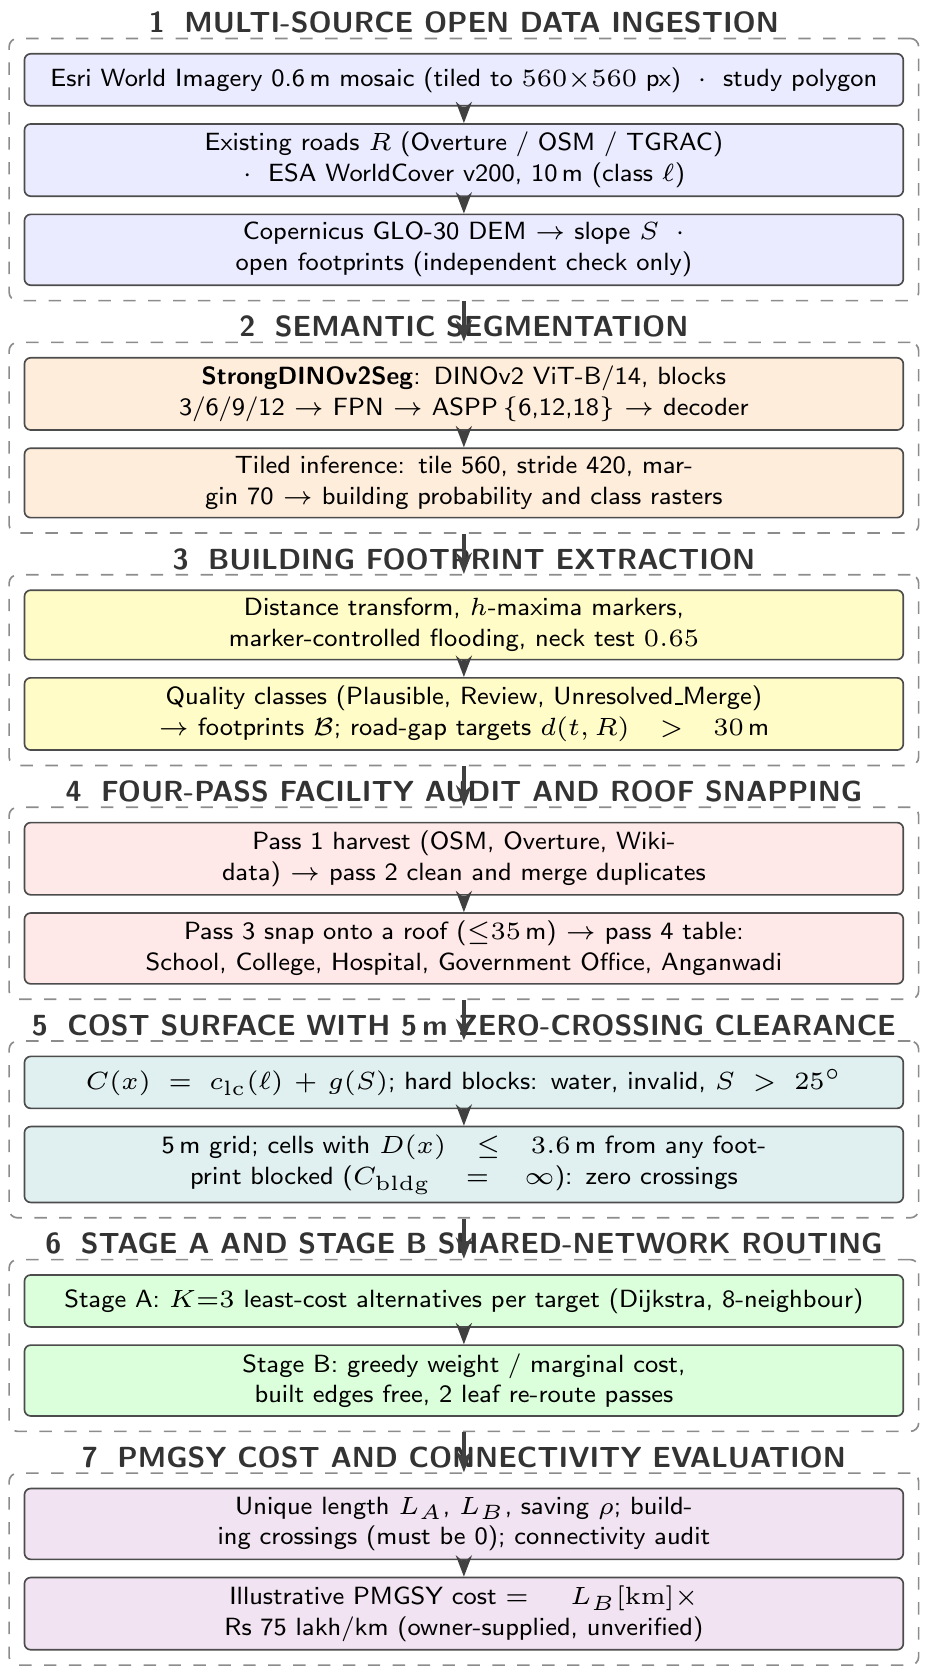
\includegraphics[width=0.5\textwidth]{figures/fig_architecture.png}
\caption{Seven-step architecture: (1)~multi-source open-data ingestion, (2)~\dinoseg{} semantic segmentation (tile 560, stride 420, margin 70), (3)~distance-transform building footprint extraction (neck ratio 0.65), (4)~four-pass multi-source facility audit and roof snapping (School, College, Hospital, Government Office, Anganwadi), (5)~cost surface with a 5~m zero-crossing clearance (3.6~m), (6)~Stage~A independent and Stage~B shared-network Dijkstra routing, (7)~PMGSY cost and connectivity evaluation.}
\label{fig:arch}
\end{figure}

\subsection{Building extraction}
\dinoseg{} is a fully fine-tuned DINOv2 ViT-B/14 encoder \cite{oquab2023dinov2}. Tokens from blocks 3, 6, 9 and 12 are projected to 256 channels, fused (FPN-style \cite{lin2017fpn}), passed through an ASPP neck (rates 6, 12, 18) \cite{chen2018deeplabv3plus} and a four-stage decoder with auxiliary heads for deep supervision \cite{lee2015dsn}. Training used LoveDA \cite{wang2021loveda} at 560~px for a scheduled 10 epochs (AdamW, cosine schedule to $10^{-7}$, encoder learning rate $\times 0.1$) with loss $0.5\,\mathrm{CE}+0.4\,\mathrm{Dice}+0.1\,\mathrm{edge}$ \cite{milletari2016vnet} and auxiliary weight 0.4. The epoch-4 checkpoint was used; the file used for the Adilabad run has SHA-256 \texttt{2e7c4646dc77ceb2\allowbreak a357f44f11cb3f7f\allowbreak f84e636871d70ba4\allowbreak c31e194e5ec00cf3}. Building instances are extracted from the predicted mask with OpenCV and NumPy: h-maxima of the distance transform give markers, a neck test (ratio 0.65) decides whether touching blobs are split, and blobs that cannot be split are flagged \textsc{Unresolved\_Merge}.

\subsection{Road-gap targets and Adilabad footprint sources}
For Adilabad the same imagery-to-footprint chain is run on Esri imagery (Section~\ref{sec:adilabad_data}), and Overture footprints serve as an independent check. Because connecting every footprint is meaningless in a built-up fabric already served by roads, only houses more than 30~m (the planner snap distance) from an existing road are routed. Planner cost grows roughly quadratically with the number of targets, which further motivates the filter; the threshold is varied (20, 30, 50~m) in Section~\ref{sec:adilabad}.

\subsection{Cost surface}
Let $\mathcal{B}$ be blocked cells (water, invalid cells, slope $>25^{\circ}$) and $\mathcal{P}$ the cells whose centre lies inside a footprint. The graph has the unblocked 10~m cells as nodes and 8-neighbour edges with no diagonal corner-cutting. The cell cost is
\begin{equation}
c(x)=\bigl[c_{\mathrm{lc}}(\ell(x))+g(s(x))\bigr]\,m(x),\qquad m(x)=\begin{cases}\mu & x\in\mathcal{P}\\ 1 & \text{otherwise,}\end{cases}
\label{eq:cell}
\end{equation}
where $\ell$ is the WorldCover class with resistance $c_{\mathrm{lc}}=8,5,3,6,2,4$ for trees, shrubland, grassland, cropland, built-up and bare/sparse land respectively (classes 10--60 in the order 10, 20, 30, 40, 50, 60), $g(s)=4\,\mathrm{clip}(s,0,10)/10$ with $s$ the slope in degrees, and $\mu=4$ is the footprint penalty. Edge weights are the mean end-cell cost times step length. Costs are ordinal planning units, not currency. In Damarakunta the penalty is lifted within a 20~m disc around the health sub-centre,  The land-cover, slope, cost and blocked-cell rasters are the inputs of the cost surface of every study area (figure~\ref{fig:flow}).whose point lies on the edge of its own footprint.

\subsection{Shared-network planner}
For each target, Stage~A computes a least-cost path to the existing road cells with Dijkstra's algorithm \cite{dijkstra1959note,hart1968astar,collischonn2000lcp} and alternatives by inflating costs along earlier paths ($K=3$ alternatives in total). Stage~B greedily selects the (target, alternative) pair with the highest weight per marginal cost
\begin{equation}
\Delta\Lcost\bigl(\pi\mid S\bigr)=\sum_{e\in\pi\setminus E_S}w(e),
\label{eq:marginal}
\end{equation}
where $E_S$ is the set of already selected edges, so built edges are free and a route may end on another route. This is the shortest-path heuristic for Steiner trees \cite{kou1981steiner,mehlhorn1988steiner} on a penalised, land-cover-weighted graph with the road network as a free sub-tree; it carries no optimality guarantee. Two passes of leaf re-routing follow. Snap distance is 30~m, search limit 1{,}500~m and attachment tolerance 15~m. Facilities are planned in a separate phase.

\subsection{Facility audit and roof snapping}
Overture Places alone mislocated or missed colleges, hospitals, offices and anganwadis, so the facilities of each area come from a four-pass audit (\texttt{scripts/audit\_facilities.py}). Pass~1 harvests candidates inside and within 500~m of the polygon from OpenStreetMap (Overpass and the Photon geocoder), Overture Places, Wikidata and Wikipedia (and, for Damarakunta, the TGRAC layers); LGD, UDISE+ and the district directories have no open query interface and were not used. Pass~2 assigns one of five categories (School, College, Hospital, Government Office, Anganwadi), removes closed or commercial records (pharmacies, laboratories, coaching centres, banks, cooperative societies), religious sites, foreign place names, placeholder coordinates shared by several differently named records, and merges duplicates of one campus across sources; every removal is logged with its reason. Pass~3 moves each survivor onto the footprint that contains it or, failing that, the nearest footprint of at least 25~m$^2$ within 35~m (a compound building up to 25~m away for a school, college or hospital), and removes facilities with no building in range. Pass~4 writes the verified table with the sources, the snap distance and a confidence label; records with a single source and a snap of more than 12~m are kept with \texttt{use\_in\_analysis}${}=$\,False and are not routed.

\subsection{Zero-crossing building clearance}
The soft footprint penalty $\mu$ in equation~\ref{eq:cell} lets a route cross a roof when the detour costs more. The proposed plan therefore uses a hard barrier on a finer grid. Each 10~m cost cell is refined to $2\times2$ cells of cell size $\Delta=5$~m with the same cost per metre, and every cell whose centre lies within $r_c=3.6$~m of any footprint is blocked (equation~\ref{eq:bldg}). Because $r_c>\Delta\sqrt2/2=3.54$~m, no step between two free cell centres can touch a footprint: a point of the step lies within $\Delta\sqrt2/2$ of one of its end points, and that end point would then have been blocked. A target sits inside its own building, so each route starts at the edge of that building and reaches the nearest free cell that is connected to the road network by a straight lane of at most the snap distance that touches no other footprint; a target with no such lane (a house enclosed by other buildings) is reported as unrouted, never routed over a roof. Lengths are measured from the building edge. Every drawn route (lane, path and attachment to a road) is finally intersected with all footprints other than its own.

\subsection{Mathematical formulation}
\paragraph{Segmentation loss.} With logits $\mathbf z$, labels $y$, class probabilities $p_{ic}$ and one-hot targets $t_{ic}$ at pixel $i$ (class 0 is ignored),
\begin{equation}
\mathcal L(\mathbf z,y)=0.5\,\mathcal L_{\mathrm{CE}}+0.4\,\mathcal L_{\mathrm{Dice}}+0.1\,\mathcal L_{\mathrm{edge}},\qquad
\mathcal L_{\mathrm{total}}=\mathcal L(\mathbf z^{\mathrm{main}},y)+0.4\sum_{j=1}^{3}\mathcal L(\mathbf z^{(j)},y),
\label{eq:loss}
\end{equation}
\begin{equation}
\mathcal L_{\mathrm{Dice}}=\frac1{|\mathcal C|}\sum_{c\in\mathcal C}\Bigl(1-\frac{2\sum_i p_{ic}t_{ic}+\varepsilon}{\sum_i p_{ic}+\sum_i t_{ic}+\varepsilon}\Bigr),\qquad
\mathcal L_{\mathrm{edge}}=\frac1{|\Omega|}\sum_{i\in\Omega}(1+4e_i)\,\mathrm{CE}_i,\quad e_i=\min\{1,\,|(K_x{*}y)_i|+|(K_y{*}y)_i|\}.
\label{eq:diceedge}
\end{equation}
Here $\mathcal C$ is the set of scored classes, $\varepsilon$ a small smoothing constant, $K_x,K_y$ the Sobel kernels, so that the edge term up-weights the cross-entropy of pixels on label boundaries by up to five; the three auxiliary heads $\mathbf z^{(j)}$ provide deep supervision.

\paragraph{Evaluation metrics.} From the confusion matrix, with $TP_c,FP_c,FN_c$ the true positives, false positives and false negatives of class $c$ and $N$ the number of labelled pixels,
\begin{equation}
\mathrm{OA}=\frac{\sum_c TP_c}{N},\quad P_c=\frac{TP_c}{TP_c+FP_c},\quad R_c=\frac{TP_c}{TP_c+FN_c},\quad F_{1,c}=\frac{2P_cR_c}{P_c+R_c}=\frac{2TP_c}{2TP_c+FP_c+FN_c},\quad \mathrm{IoU}_c=\frac{TP_c}{TP_c+FP_c+FN_c},
\label{eq:metrics}
\end{equation}
and $P$, $R$, $F_1$ (the Dice coefficient) and $\mathrm{mIoU}=|\mathcal C|^{-1}\sum_{c\in\mathcal C}\mathrm{IoU}_c$ are the macro averages over the scored classes. Because $F_{1,c}$ equals the per-class Dice score, the reported F1-score is the mean Dice.

\paragraph{Terrain.} Slope is taken from the Copernicus GLO-30 elevation $z$ with the Sobel gradient at the DEM spacing $\Delta_z=30$~m, resampled bilinearly to the planning grid:
\begin{equation}
\partial_x z\approx\frac{(K_x{*}z)}{8\Delta_z},\quad \partial_y z\approx-\frac{(K_y{*}z)}{8\Delta_z},\quad S=\arctan\sqrt{(\partial_x z)^2+(\partial_y z)^2},\quad p_S=100\tan S,
\label{eq:slope}
\end{equation}
with $S$ the slope in degrees and $p_S$ the equivalent percentage slope reported in the comparison table. The cost uses the linear ramp $g(S)=w_s\min(S,S_{\mathrm{ref}})/S_{\mathrm{ref}}$ with $w_s=4$ and $S_{\mathrm{ref}}=10^{\circ}$, and cells with $S>S_{\lim}=25^{\circ}$ are blocked; no separate IRC slope-penalty factor is applied.

\paragraph{Composite cost and clearance barrier.} With $c_{\mathrm{lc}}(\ell)$ the WorldCover resistance (equation~\ref{eq:cell}, so the land-cover weight is $w_{\mathrm{lc}}=1$) and $D(x)$ the Euclidean distance from the centre of cell $x$ to the nearest footprint (zero inside a footprint),
\begin{equation}
C(x)=c_{\mathrm{lc}}(\ell(x))+g(S(x))+C_{\mathrm{bldg}}(x),\qquad C_{\mathrm{bldg}}(x)=\begin{cases}\infty & D(x)\le r_c\\ 0 & \text{otherwise,}\end{cases}\qquad r_c=3.6\ \mathrm{m},\ \Delta=5\ \mathrm{m}.
\label{eq:bldg}
\end{equation}
The ten-metre comparison baseline instead multiplies the cost of cells whose centre lies in a footprint by $\mu=4$ (equation~\ref{eq:cell}).

\paragraph{Graph and routing objectives.} The graph has the free cells as nodes and 8-neighbour edges, a diagonal step being allowed only if both orthogonal neighbours are free. The weight of an edge $(u,v)$ is
\begin{equation}
w(u,v)=d(u,v)\,\frac{C(u)+C(v)}{2},\qquad d(u,v)=\begin{cases}\Delta&\text{cardinal step}\\ \sqrt2\,\Delta&\text{diagonal step.}\end{cases}
\label{eq:edge}
\end{equation}
Stage~A gives every target $t$ the independent least-cost path $\pi_t^{A}=\arg\min_{\pi:\,t\to R}\sum_{e\in\pi}w(e)$ to the existing road cells $R$ (Dijkstra), and two further alternatives that multiply $w(e)$ by $\lambda\in\{3,8\}$ on cells within $20$~m of the earlier paths and overlap them by at most 80\%. Stage~B starts from $E_S=\emptyset$ and repeatedly serves the target and route with the highest weight per marginal cost,
\begin{equation}
(t^\star,\pi^\star)=\arg\max_{t\in U,\ \pi\in\Pi_t\cup\{\pi_t^{\mathrm{net}}\}}\frac{\omega_t}{\Delta\Lcost(\pi\mid S)},\qquad
\Delta\Lcost(\pi\mid S)=\sum_{e\in\pi\setminus E_S}w(e),
\label{eq:stageb}
\end{equation}
where $U$ is the set of unserved targets, $\Pi_t$ the Stage~A alternatives, $\pi_t^{\mathrm{net}}$ the least-cost path to the roads together with the routes already selected, and $\omega_t$ the priority weight ($4$ for hospitals and health centres, $3$ for schools, colleges and anganwadis, $2$ for government offices, $1$ for houses). A built edge $e\in E_S$ thus costs nothing again, which is a discount factor $\alpha=0$ on $E_S$; no intermediate $\alpha\in(0,1)$ is used. With $L(\cdot)$ the total length of the unique edges of a route set (shared edges once),
\begin{equation}
\rho=\frac{L_A-L_B}{L_A}\times100\%,\qquad L_A=L\bigl(\{\pi_t^A\}\bigr),\quad L_B=L(E_S),\qquad X=\sum_{r}\Bigl|r\cap\bigcup_{b\ne b_r}b\Bigr|=0,
\label{eq:saving}
\end{equation}
where $X$ is the length of routes inside footprints other than the route's own building $b_r$ (zero by construction under equation~\ref{eq:bldg}).

\paragraph{Illustrative cost.} The capital cost is
\begin{equation}
\mathrm{Cost}_{\mathrm{INR\ lakh}}=L_B[\mathrm{km}]\times c_{\mathrm{PMGSY}},\qquad c_{\mathrm{PMGSY}}=75\ \text{lakh/km}\ (\text{range }60\text{--}90),
\label{eq:cost}
\end{equation}
with 1 lakh $=10^{5}$~INR. The rate was supplied by the project owner as PMGSY-based and has not been verified against a PMGSY document or a State Schedule of Rates, so the cost is illustrative and not an engineering estimate.

\subsection{Algorithms}
\begin{algorithm}[t]
\caption{Tiled \dinoseg{} inference and distance-transform building extraction (\texttt{run\_tiled\_inference.py}, \texttt{extract\_buildings\_v8.py})}
\label{alg:extract}
\begin{algorithmic}[1]
\Require mosaic $I$ (0.6~m), checkpoint $\theta$, tile $T=560$, stride $s=420$, margin $m=70$, neck ratio $\eta=0.65$, seed height $h=0.3$~m
\Ensure footprints $\mathcal B$ with quality classes
\State \textbf{assert} $s\le T-2m$ \Comment{no gaps between tile centres}
\For{each tile of size $T\times T$ at stride $s$}
  \State $p\gets\mathrm{softmax}(f_\theta(\text{tile}))$; write class $\arg\max p$ and $p_{\mathrm{bldg}}$ for the tile centre (drop $m$ px at inner edges)
\EndFor
\State $M\gets(\text{class}=\text{building})\wedge\lnot\text{no-data}$; drop components smaller than 6~m$^2$
\For{each connected component $K$ of $M$}
  \State $D\gets\mathrm{EDT}(K)$ (smoothed, $\sigma=1$ px); markers $\gets$ $h$-maxima of $D$ with height $h$
  \State pieces $\gets$ marker-controlled flooding of $-D$ (only if area $\ge 40$~m$^2$)
  \For{each adjacent piece pair $(a,b)$}
    \State $r_{ab}\gets D_{\mathrm{saddle}}/\min(D_a^{\max},D_b^{\max})$
    \If{$r_{ab}>\eta$ \textbf{or} a piece is smaller than 12~m$^2$} merge $a,b$ \Comment{no real neck}
    \EndIf
  \EndFor
\EndFor
\State polygonise; flag \textsc{Unresolved\_Merge} if area $>4\times$ the median compact roof; assign \textsc{Plausible} / \textsc{Review} / \textsc{Small} by confidence and shape
\State \Return $\mathcal B$
\end{algorithmic}
\end{algorithm}

\begin{algorithm}[t]
\caption{Cost surface with zero-crossing clearance and two-stage routing (\texttt{clearance.py}, \texttt{plan\_network\_v2.py})}
\label{alg:route}
\begin{algorithmic}[1]
\Require land cover $\ell$, DEM $z$, roads $R$, footprints $\mathcal B$, targets $\mathcal T$ (road-gap houses and verified facilities with weights $\omega_t$), $\Delta=5$~m, $r_c=3.6$~m, $K=3$
\Ensure route sets $\{\pi_t^A\}$, $E_S$ and lengths $L_A$, $L_B$, saving $\rho$, cost
\State $S\gets$ slope of $z$ (equation~\ref{eq:slope}); $C_0(x)\gets c_{\mathrm{lc}}(\ell(x))+g(S(x))$; block water, invalid cells and $S>25^{\circ}$
\State refine $C_0$ from 10~m to $\Delta=5$~m (same cost per metre); $D\gets\mathrm{EDT}(\mathcal B)$; $C(x)\gets\infty$ where $D(x)\le r_c$
\State keep the free cells connected to a road cell; edge weights $w$ by equation~\ref{eq:edge}
\For{each target $t\in\mathcal T$}
  \State entrance $e_t\gets$ point of the target's building edge nearest to a free cell $s_t$; require a lane $e_t\to s_t$ of at most 30~m that touches no other footprint, else mark $t$ unrouted
  \State $\Pi_t\gets K$ Dijkstra alternatives from $s_t$ to $R$ (corridor inflation $\lambda\in\{3,8\}$, 20~m, overlap $\le 80\%$); $\pi_t^A\gets$ first alternative
\EndFor
\State $L_A\gets L(\{\pi_t^A\})$; $U\gets$ routed targets; $E_S\gets\emptyset$
\While{$U\ne\emptyset$}
  \For{each $t\in U$} add the least-cost path $\pi_t^{\mathrm{net}}$ to $R\cup E_S$ to the candidates $\Pi_t$ \EndFor
  \State $(t^\star,\pi^\star)\gets\arg\max\ \omega_t/\Delta\Lcost(\pi\mid S)$ (equation~\ref{eq:stageb}); $E_S\gets E_S\cup\pi^\star$; $U\gets U\setminus\{t^\star\}$
\EndWhile
\State two leaf re-route passes: replace a route that no other route uses if it has become cheaper given the others
\State verify $X=0$ (equation~\ref{eq:saving}); $L_B\gets L(E_S)$; $\rho\gets 100(L_A-L_B)/L_A$; cost by equation~\ref{eq:cost}
\end{algorithmic}
\end{algorithm}

\subsection{Baselines, scenarios and metrics}
Four baselines are compared: straight lines, independent least-cost routes, a length-only control (cost surface replaced by distance) and a roads-only shared reference (routes may share edges only with the existing road network). The saving against independent routing is $\rho=(L_{\mathrm{ind}}-L)/L_{\mathrm{ind}}$, with $L$ the unique network length (shared edges counted once). The exposure metrics are the number of routes crossing another house's footprint and the route length inside other footprints. The footprint penalty is varied ($\mu\in\{1,4,20,100\}$, with a variant in which footprints are buffered by 7.1~m). For omissions, a target set $M$ is removed from the targets and from the penalty layer (a missed detection is absent from both), and the planner is re-run; random draws use seeds 1--5. Coverage, unserved households, change in unique length and length per routed target are reported.

\section{Results: Damarakunta}\label{sec:damar}
\subsection{Detection}
On the 1{,}669-image LoveDA validation split (560~px, seven scored classes) the epoch-4 checkpoint reached 53.8\% mIoU, 68.9\% Dice and 71.3\% pixel accuracy, with 72.4\% macro precision and 66.9\% macro recall; for the Building class IoU is 54.0\%, precision 62.1\% and recall 80.6\% (table~\ref{tab:seg}). These are source-domain figures, not accuracy on Damarakunta. Against Google Open Buildings v3 as a proxy (not ground truth), 118 of the 165 in-boundary candidates agree (71.5\%).

\begin{table}[t]
\caption{Detection evaluation. Top: LoveDA validation (source domain); precision and recall are macro-averages over the seven scored classes. Bottom: agreement of the 165 Damarakunta candidates with Open Buildings v3 (a proxy, not accuracy).}
\label{tab:seg}
\centering
\small
\begin{tabular}{@{}lrrrrr@{}}
\toprule
\multicolumn{6}{@{}l}{\textit{LoveDA validation split (\%)}}\\
 & mIoU & Dice & Pixel acc. & Precision & Recall\\
\midrule
StrongDINOv2Seg & 53.8 & 68.9 & 71.3 & 72.4 & 66.9\\
\quad Building class & 54.0 & 70.1 & --- & 62.1 & 80.6\\
\midrule
\multicolumn{6}{@{}l}{\textit{Damarakunta candidates vs.\ Open Buildings v3}}\\
Class & Candidates & Agree & Disagree & \multicolumn{2}{c}{Agreement (\%)}\\
\midrule
All & 165 & 118 & 47 & \multicolumn{2}{c}{71.5}\\
\textsc{Plausible} & 71 & 51 & 20 & \multicolumn{2}{c}{71.8}\\
\textsc{Review} & 32 & 14 & 18 & \multicolumn{2}{c}{43.8}\\
\textsc{Unresolved\_Merge} & 62 & 53 & 9 & \multicolumn{2}{c}{85.5}\\
\bottomrule
\end{tabular}
\end{table}

\subsection{Shared network and footprint penalty}
Independent least-cost routes for the 163 houses total 10{,}045~m, but because neighbouring houses re-trace the same corridors the unique built length is 6{,}753~m (table~\ref{tab:routing}, figure~\ref{fig:routing}a). The two-stage plan reduces this to 5{,}069~m, a saving of 24.9\%; all 163 houses and five facilities are connected. The length-only control is 3.4\% \emph{longer} in unique length than independent cost-surface routing, and the roads-only shared reference saves 22.6\%, so most of the saving comes from sharing and a further 2.3 percentage points from sharing between new routes.

The penalty trades length for exposure (figure~\ref{fig:routing}b). With $\mu=1$ the plan is shortest (4{,}705~m) but 56 routes pass through other houses (660~m inside footprints). With $\mu=4$ it is 7.7\% longer while crossings halve to 28 routes and 209~m. Buffering footprints by 7.1~m with $\mu=20$ or 100 lowers crossings further (19 routes) at 6{,}190--6{,}238~m.

\begin{table}[t]
\caption{Damarakunta routing, 163 houses ($\mu=4$ unless stated). Total length counts every route; unique length counts shared edges once; $\rho$ is the saving in unique length against independent routes.}
\label{tab:routing}
\centering
\footnotesize
\begin{tabular}{@{}>{\raggedright\arraybackslash}p{4.3cm}rrrrr@{}}
\toprule
Strategy & Total (m) & Unique (m) & $\rho$ (\%) & Routes crossing & In footprints (m)\\
\midrule
Straight line (2 targets infeasible) & 8{,}092.3 & --- & --- & 60 & 1{,}453.2\\
Independent least-cost routes & 10{,}045.4 & 6{,}753.1 & 0.0 & 46 & 328.3\\
Length-only control & 9{,}166.3 & 6{,}979.8 & $-3.4$ & 64 & 1{,}615.8\\
Roads-only shared reference & 5{,}229.3 & 5{,}229.3 & 22.6 & 29 & 216.1\\
\textbf{Two-stage plan (proposed)} & \textbf{5{,}069.0} & \textbf{5{,}069.0} & \textbf{24.9} & \textbf{28} & \textbf{209.1}\\
\midrule
\multicolumn{6}{@{}l}{\textit{No footprint penalty ($\mu=1$)}}\\
Independent least-cost routes & 9{,}595.9 & 6{,}921.3 & 0.0 & 63 & 1{,}423.1\\
Two-stage plan & 4{,}705.5 & 4{,}705.4 & 32.0 & 56 & 660.1\\
\midrule
\multicolumn{6}{@{}l}{\textit{Buffered footprints (7.1~m), two-stage plan}}\\
Penalty $\mu=20$ & --- & 6{,}238.1 & 18.5 & 19 & 147.9\\
Penalty $\mu=100$ & --- & 6{,}190.3 & 18.9 & 19 & 144.8\\
\bottomrule
\end{tabular}
\end{table}

\begin{figure}[t]
\centering
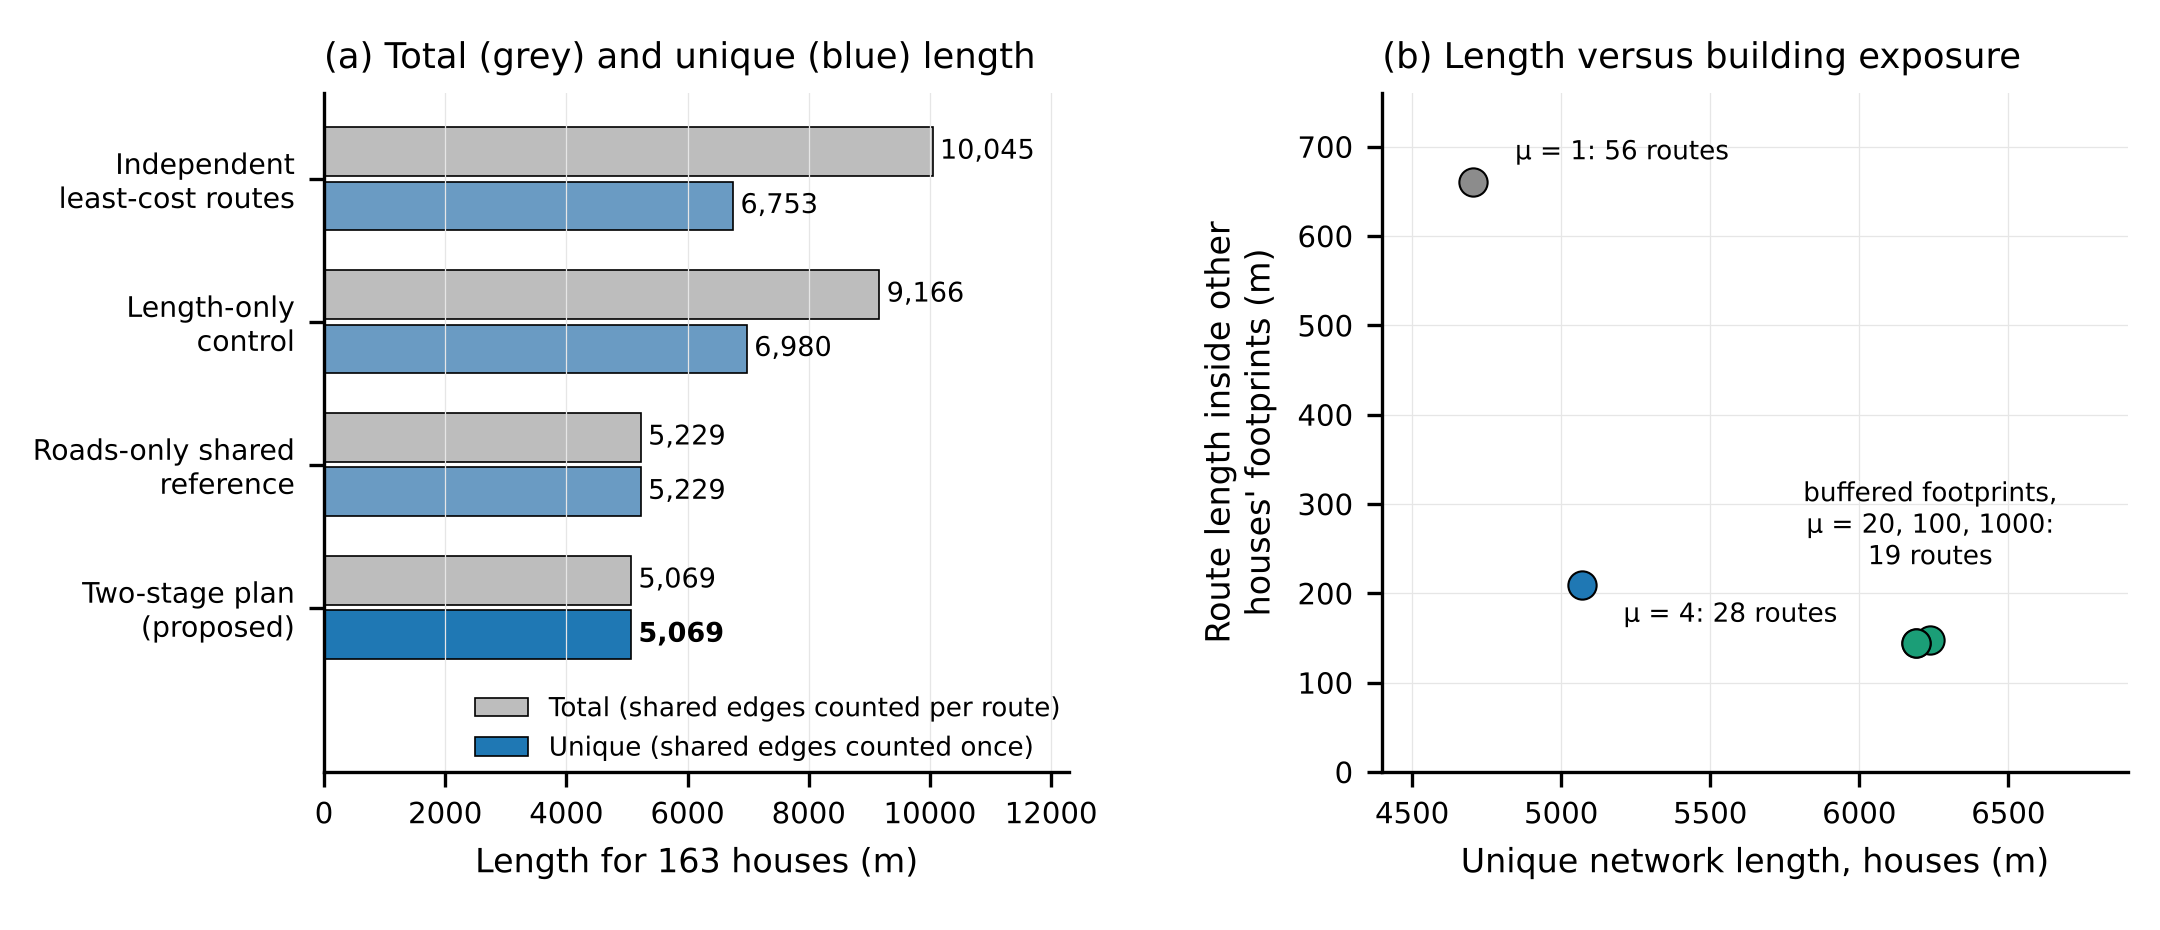
\includegraphics[width=\textwidth]{figures/fig3_routing.png}
\caption{Damarakunta routing results for 163 houses. (a)~Total and unique corridor length by strategy. (b)~Unique network length against route length inside other houses' footprints for $\mu=1$, $\mu=4$ and buffered footprints with large penalties.}
\label{fig:routing}
\end{figure}

\subsection{Impact of building omissions}
Table~\ref{tab:omission} and figure~\ref{fig:omission} summarise the omission analysis against the 5{,}069~m baseline. Missing buildings make the plan \emph{shorter}: 10\% random omission (16 houses) understates length by 7.6\%, 20\% by 16.9\%, omission of the smallest quarter by 25.1\% and omission of all merged blobs by 29.4\%. At the same time $U$ households lose access: 16 and 33 for random 10\% and 20\% omission, 41 for the smallest quarter and 62 (38.0\%) for merged blobs. A planner reading only total length would therefore underfund the scheme. Random additions lengthen the plan by 8.6\% and 15.8\%. The saving $\rho$ stays within 24.9--26.6\% across omissions, so the benefit of sharing is robust to inventory error.

\begin{table}[t]
\caption{Impact of simulated omissions and additions, Damarakunta. Baseline 5{,}069.0~m, 163 routed. Random scenarios are means of five draws. $U$: households without a route; $\kappa$: coverage; $\delta_L$: change in unique length; $\bar\ell$: length per routed target; $\rho$: saving against independent routing.}
\label{tab:omission}
\centering
\small
\begin{tabular}{@{}lrrrrrrr@{}}
\toprule
Scenario & Routed & $U$ & $\kappa$ (\%) & $L$ (m) & $\delta_L$ (\%) & $\bar\ell$ (m) & $\rho$ (\%)\\
\midrule
Baseline & 163 & 0 & 100.0 & 5{,}069.0 & 0.0 & 31.1 & 24.9\\
Omit 10\% (random) & 147.0 & 16 & 90.2 & 4{,}684.4 & $-7.6$ & 31.9 & 25.1\\
Omit 20\% (random) & 130.0 & 33 & 79.8 & 4{,}211.5 & $-16.9$ & 32.4 & 24.9\\
Omit smallest 10\% & 146 & 17 & 89.6 & 4{,}648.6 & $-8.3$ & 31.8 & 24.9\\
Omit smallest 25\% & 122 & 41 & 74.8 & 3{,}798.3 & $-25.1$ & 31.1 & 25.6\\
Omit merged blobs & 101 & 62 & 62.0 & 3{,}579.0 & $-29.4$ & 35.4 & 26.6\\
\midrule
Add 10\% (random) & 177.4 & --- & --- & 5{,}502.4 & $+8.6$ & 31.0 & 25.6\\
Add 20\% (random) & 190.6 & --- & --- & 5{,}868.3 & $+15.8$ & 30.8 & 25.4\\
\bottomrule
\end{tabular}
\end{table}

\begin{figure}[t]
\centering
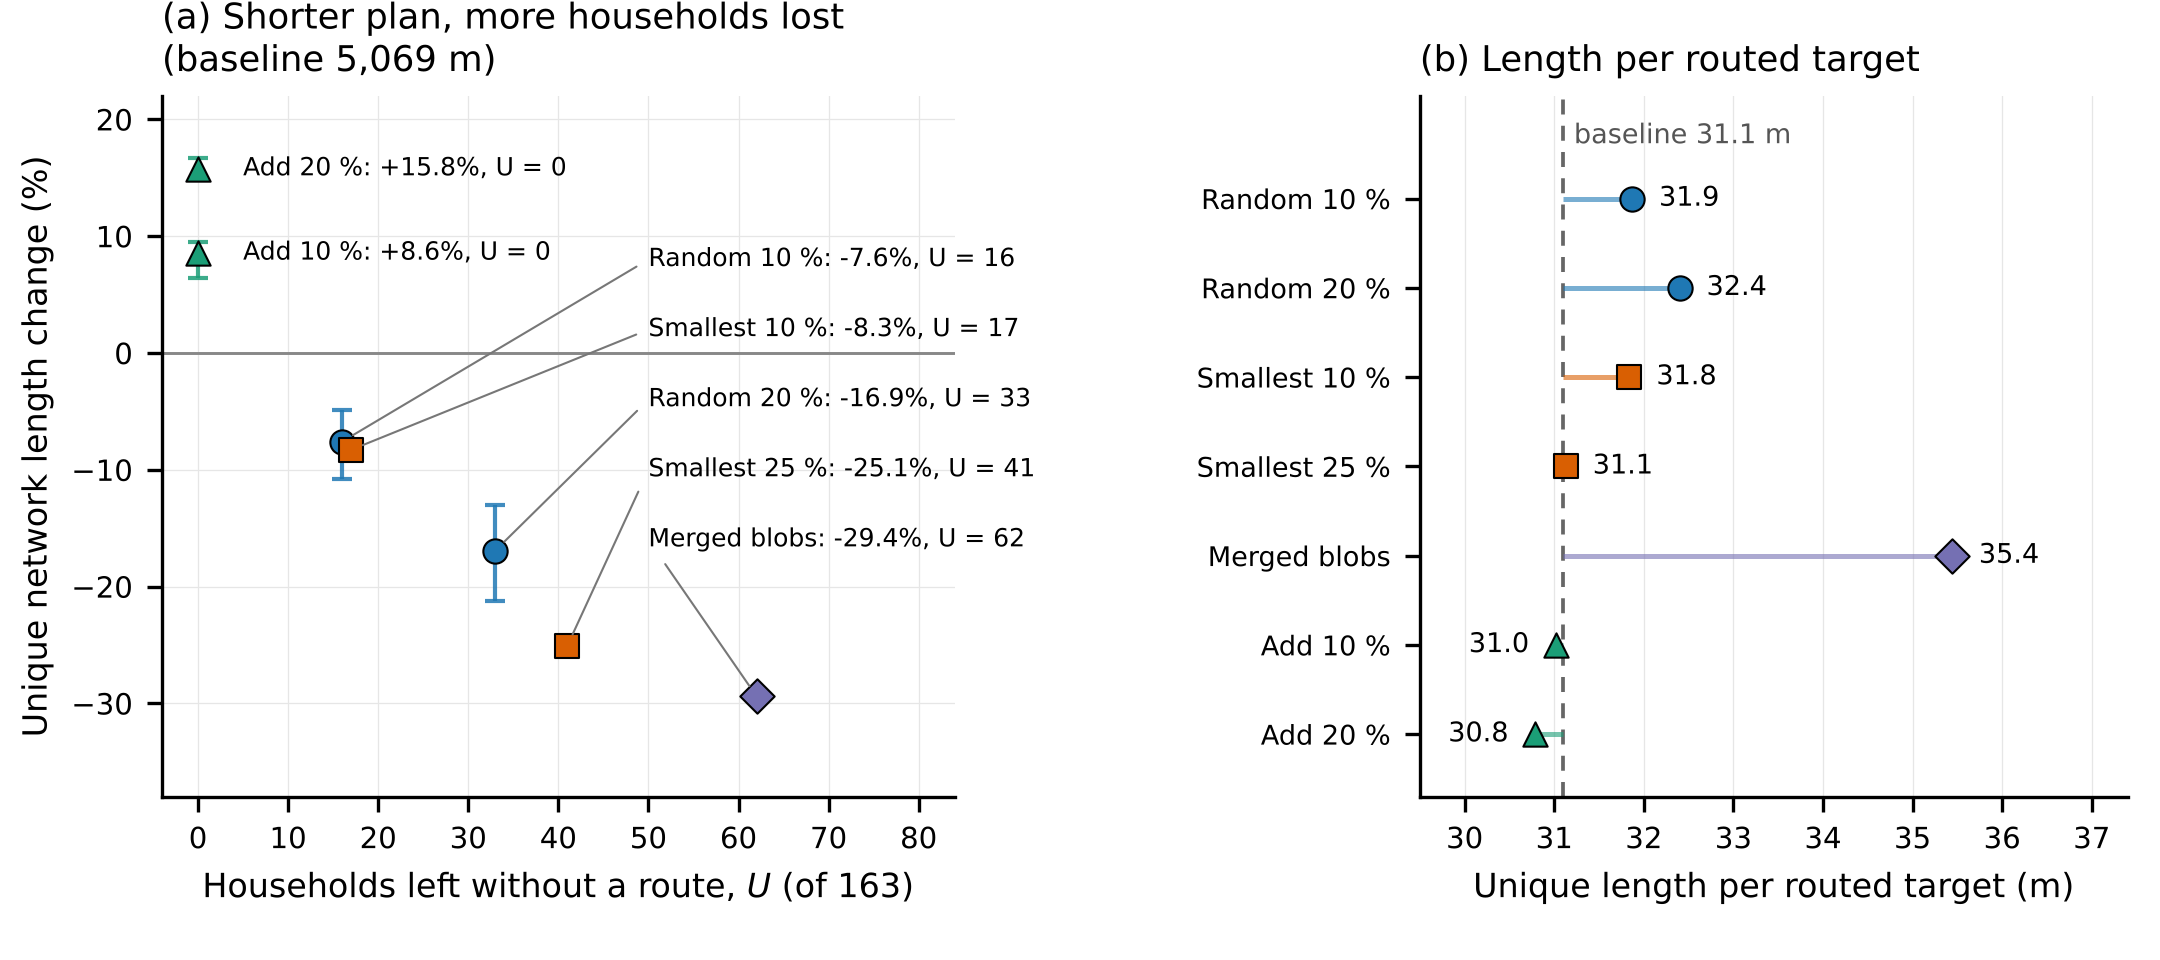
\includegraphics[width=\textwidth]{figures/fig4_omission.png}
\caption{Damarakunta omission sensitivity (163 baseline targets, 5{,}069~m; random scenarios are five draws with min--max bars). (a)~Change in unique length against households left without a route. (b)~Unique length per routed target.}
\label{fig:omission}
\end{figure}

\section{Results: transfer to Adilabad Urban}\label{sec:adilabad}
\subsection{Road-gap targets and routing}
\emph{End-to-end run (\dinoseg{} footprints).} Of the 2{,}690 footprints of at least 30~m$^2$, 345 lie more than 30~m from a road and form the targets (Damarakunta: 163). The planner routes all 345. Independent least-cost routes total 23{,}312.5~m (unique 21{,}440.8~m); the two-stage plan needs 18{,}288.7~m, a saving of 14.7\% (table~\ref{tab:adilabad}; the routes are drawn in figure~\ref{fig:flow}). The roads-only shared reference saves 2.3\% and the length-only control 6.9\%, so almost all of the saving comes from sharing among new routes. Exposure: 54 of 345 routes (15.7\%) cross another footprint (398.0~m), against 28 of 163 (17\%) in Damarakunta.

These numbers must be read with the extraction quality in mind. More than half of the instances (1{,}580 of 2{,}769) are \textsc{Unresolved\_Merge} blobs with a median area of 1{,}125.5~m$^2$: in the dense fabric the segmenter merges neighbouring roofs, so the 345 targets are built-up units rather than houses, and the footprint penalty acts on merged blocks. No reference mask exists for Adilabad, so detection accuracy there is not known.

\emph{Open-footprint check.} With 874 road-gap targets (873 routed) among 18{,}242 Overture footprints (median footprint 139.6~m$^2$, median distance to the nearest road 42.3~m), independent routes total 56{,}308.0~m (unique 46{,}419.2~m) and the two-stage plan 34{,}358.8~m, a saving of 26.0\%; the roads-only reference saves 2.9\% and the length-only control 5.7\%; 332 of 873 routes (38\%) cross another footprint (2{,}041.1~m). The facility phase connects 71 verified facilities with 1{,}090.1~m of unique corridor.

Both Adilabad variants agree that sharing helps (14.7\% and 26.0\%) and that a roads-only reference does not (2.3\% and 2.9\%, against 22.6\% in Damarakunta), but they differ in the size of the saving. This is consistent with fewer, more widely spaced targets (345 against 874) offering less opportunity to share, an explanation that was not tested. The comparison is between two footprint sources, not a validation of either.

\begin{table}[t]
\caption{Cross-settlement comparison under the same cost surface and solver. ``Seg.'' = \dinoseg{} footprints on Esri imagery; ``open'' = Overture footprints. Targets are defined by different rules (all candidates in Damarakunta, road-gap houses in Adilabad).}
\label{tab:adilabad}
\centering
\footnotesize
\begin{tabular}{@{}>{\raggedright\arraybackslash}p{5.6cm}rrr@{}}
\toprule
Metric & Damarakunta & Adilabad seg. & Adilabad open\\
\midrule
Study area (km$^2$) & 18.47 & 17.75 & 17.75\\
Targets / routed & 163 / 163 & 345 / 345 & 874 / 873\\
Independent routes, unique (m) & 6{,}753.1 & 21{,}440.8 & 46{,}419.2\\
Length-only control, unique (m) & 6{,}979.8 & 19{,}961.2 & 43{,}787.2\\
Roads-only shared reference, unique (m) & 5{,}229.3 & 20{,}947.0 & 45{,}058.9\\
\textbf{Two-stage plan, unique (m)} & \textbf{5{,}069.0} & \textbf{18{,}288.7} & \textbf{34{,}358.8}\\
Saving vs.\ independent (\%) & 24.9 & 14.7 & 26.0\\
Roads-only shared saving (\%) & 22.6 & 2.3 & 2.9\\
Unique length per routed house (m) & 31.1 & 53.0 & 39.4\\
Routes crossing other footprints & 28 of 163 & 54 of 345 & 332 of 873\\
Length inside other footprints (m) & 209.1 & 398.0 & 2{,}041.1\\
$\mu=1\rightarrow4$: unique length change (\%) & $+7.7$ & $+9.2$ & $+13.3$\\
$\mu=1\rightarrow4$: routes crossing & 56 $\rightarrow$ 28 & 138 $\rightarrow$ 54 & 618 $\rightarrow$ 332\\
10\% random omission: change (\%) / unserved & $-7.6$ / 16 & $-8.8$ / 34 & $-7.6$ / 88\\
20\% random omission: change (\%) / unserved & $-16.9$ / 33 & $-18.3$ / 69 & $-15.0$ / 176\\
Smallest-25\% omission: change (\%) / unserved & $-25.1$ / 41 & $-21.2$ / 87 & $-21.2$ / 220\\
\bottomrule
\end{tabular}
\end{table}
\subsection{Robustness}
\emph{Footprint penalty.} Raising $\mu$ from 1 to 4 lengthens the unique network by 9.2\% and removes 84 crossing routes (138 to 54); $\mu=20$ and 100 give 19{,}777.0~m and 19{,}924.5~m with 49 and 48 routes crossing, and buffered footprints give 22{,}757.0~m and 23{,}475.5~m with 7 crossing each (table~\ref{tab:sens}, figure~\ref{fig:adilsens}a). The saving against independent routing stays between 10.1\% and 17.7\% across all settings (open footprints: 17.8\% to 30.8\%, table~\ref{tab:sens_open}).

\emph{Road-gap threshold.} Targets defined as houses more than 20, 30 or 50~m from a road number 750, 345 and 129 and give savings of 10.6\%, 14.7\% and 18.5\% (open footprints: 2{,}190, 874 and 296 targets; 21.9\%, 26.0\% and 29.5\%). The saving therefore depends on the target definition, which should be reported with any such result.

\emph{Omissions.} Random omission of 10\% and 20\% (five seeds) changes unique length by $-8.8\%$ (range $-11.7$ to $-6.5$) and $-18.3\%$ ($-21.9$ to $-15.8$), leaving 34 and 69 targets unserved; single-run smallest-10\% and smallest-25\% omissions give $-8.0\%$ and $-21.2\%$ (35 and 87 unserved). As in Damarakunta and in the open-footprint check, missing buildings shorten the plan while stranding households, and the saving stays at 12.6--14.1\%. With open footprints the same scenarios give $-7.6\%$, $-15.0\%$, $-7.9\%$ and $-21.2\%$ and a saving of 23.8--25.2\%. Merged-blob and addition scenarios were not defined for Adilabad.

\begin{table}[t]
\caption{Adilabad sensitivity, \dinoseg{} footprints (345 targets unless stated). Top: footprint-penalty settings. Bottom: road-gap threshold.}
\label{tab:sens}
\centering
\footnotesize
\begin{tabular}{@{}lrrrrr@{}}
\toprule
Setting & Unique (m) & $\rho$ (\%) & Crossing routes & In footprints (m) & Targets\\
\midrule
Centre-in-footprint, $\mu=1$ & 16{,}740.5 & 17.7 & 138 & 1{,}479.8 & 345\\
Centre-in-footprint, $\mu=4$ & 18{,}288.7 & 14.7 & 54 & 398.0 & 345\\
Centre-in-footprint, $\mu=20$ & 19{,}777.0 & 12.5 & 49 & 356.4 & 345\\
Centre-in-footprint, $\mu=100$ & 19{,}924.5 & 12.2 & 48 & 343.2 & 345\\
Buffered 7.1~m, $\mu=20$ & 22{,}757.0 & 10.1 & 7 & 57.9 & 345\\
Buffered 7.1~m, $\mu=100$ & 23{,}475.5 & 10.6 & 7 & 55.7 & 345\\
\midrule
Gap $>20$~m & 30{,}621.7 & 10.6 & 69 & 442.8 & 750\\
Gap $>30$~m (primary) & 18{,}288.7 & 14.7 & 54 & 398.0 & 345\\
Gap $>50$~m & 9{,}155.2 & 18.5 & 28 & 251.9 & 129\\
\bottomrule
\end{tabular}
\end{table}

\begin{table}[t]
\caption{Adilabad sensitivity, open Overture footprints (874 targets, 873 routed). Top: footprint-penalty settings. Bottom: road-gap threshold.}
\label{tab:sens_open}
\centering
\footnotesize
\begin{tabular}{@{}lrrrrr@{}}
\toprule
Setting & Unique (m) & $\rho$ (\%) & Crossing routes & In footprints (m) & Targets\\
\midrule
Centre-in-footprint, $\mu=1$ & 30{,}335.7 & 30.8 & 618 & 4{,}893.0 & 874\\
Centre-in-footprint, $\mu=4$ & 34{,}358.8 & 26.0 & 332 & 2{,}041.1 & 874\\
Centre-in-footprint, $\mu=20$ & 37{,}024.1 & 22.8 & 271 & 1{,}687.4 & 874\\
Centre-in-footprint, $\mu=100$ & 37{,}513.9 & 21.7 & 275 & 1{,}744.8 & 874\\
Buffered 7.1~m, $\mu=20$ & 42{,}071.9 & 20.1 & 231 & 1{,}397.2 & 874\\
Buffered 7.1~m, $\mu=100$ & 44{,}094.6 & 17.8 & 221 & 1{,}310.5 & 874\\
\midrule
Gap $>20$~m & 65{,}204.4 & 21.9 & 815 & 4{,}543.9 & 2{,}190\\
Gap $>30$~m (primary) & 34{,}358.8 & 26.0 & 332 & 2{,}041.1 & 874\\
Gap $>50$~m & 15{,}880.9 & 29.5 & 126 & 809.9 & 296\\
\bottomrule
\end{tabular}
\end{table}

\begin{figure}[t]
\centering
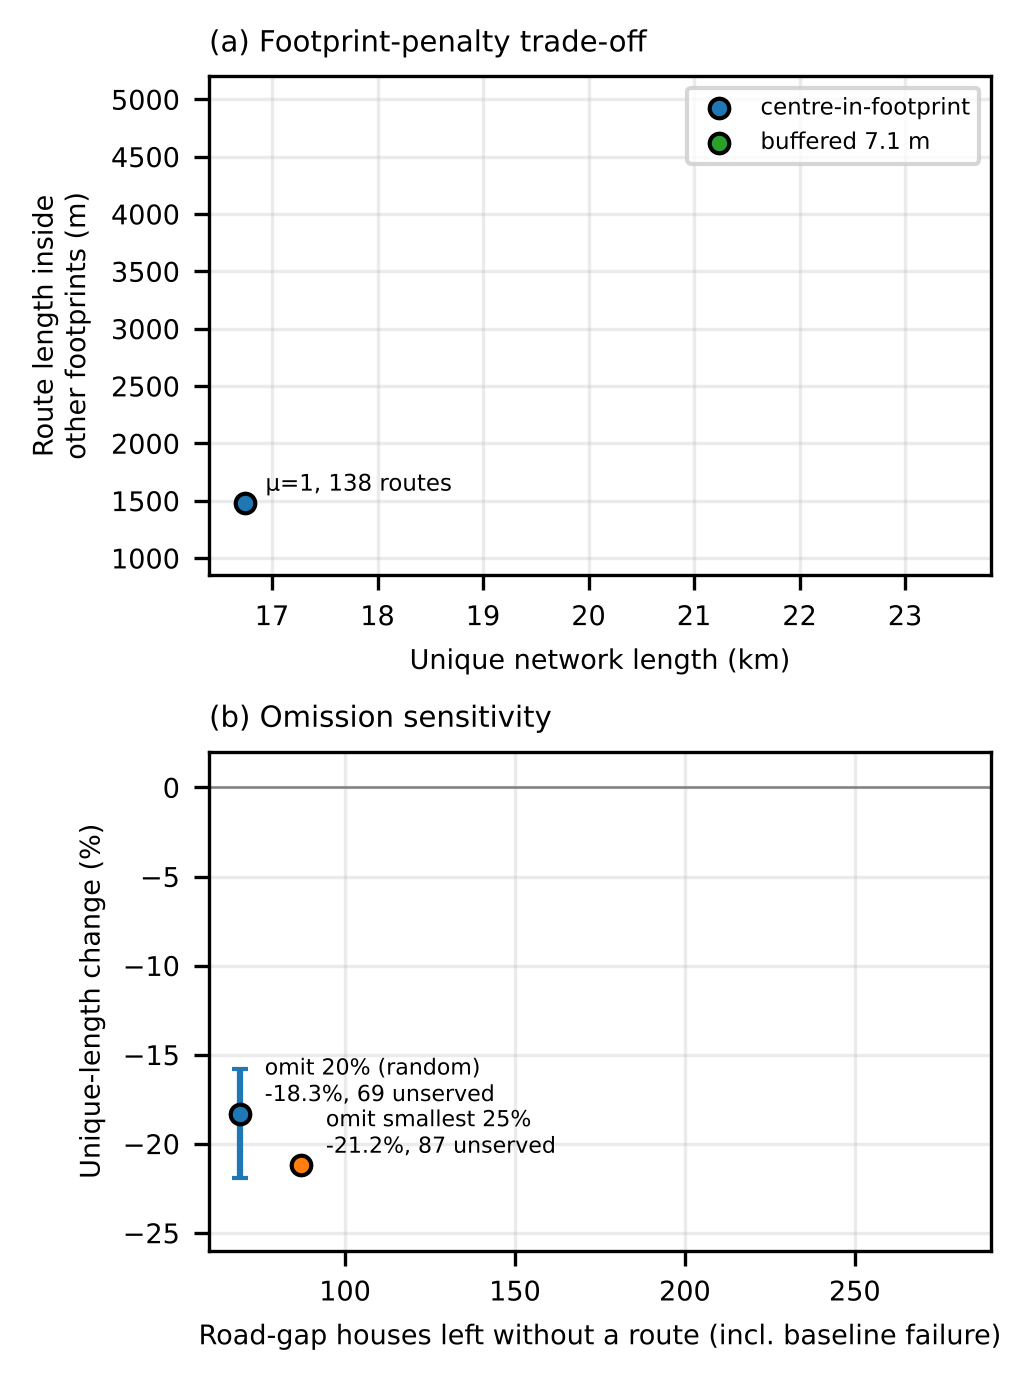
\includegraphics[width=0.5\textwidth]{figures/adilabad_seg_sens_col.png}
\caption{Adilabad sensitivity (\dinoseg{} footprints). (a)~Footprint-penalty trade-off between unique network length and route length inside other footprints. (b)~Omission sensitivity (random: mean and min--max over five seeds; smallest-$q$: single run).}
\label{fig:adilsens}
\end{figure}

\section{Results: four study areas with zero-crossing clearance}\label{sec:four}
Figure~\ref{fig:flow} follows the chain of figure~\ref{fig:arch} for the four study areas, from the Telangana locator through the input imagery and roads, the extracted footprints and verified facilities, to the planned network. Table~\ref{tab:four} collects every metric of the four areas in one place; it is regenerated by \texttt{scripts/run\_village\_pipeline.py --compare-all}, and a red \pending{value} marks a number not yet computed on the machine that wrote the table. The Adilabad column uses the updated settlement boundary (a derived built-up extent of Adilabad town) and the segmentation footprints of that boundary, so it is not the 2018 mandal experiment of the preceding sections.

On the 5~m clearance grid, Stage~B shortens the unique network relative to the independent Stage~A routes by Damarakunta 21.0\%, Adilabad 12.2\%, Aswaraopeta 25.3\%, Alampur 16.2\%. Building crossings are zero in every area by construction and were verified by intersecting every drawn route with all footprints, whereas the ten-metre soft-penalty plan ($\mu=4$) still leaves routes across other footprints (Damarakunta 28, Adilabad 99, Aswaraopeta 157, Alampur 5 routes, respectively). Targets with no free lane to the road network are reported as unrouted rather than routed over a roof, so the routed counts in table~\ref{tab:four} are below the target counts where buildings enclose a house. The segmentation rows are model-level: they are the LoveDA validation scores of the one checkpoint used for all four areas, not accuracy on any of the four areas, for which no surveyed reference exists. Costs use the owner-supplied, unverified PMGSY-based rate of Rs 75 lakh/km and are illustrative.

\begin{figure*}[p]
\centering
\IfFileExists{figures/fig_flow_study_areas.png}{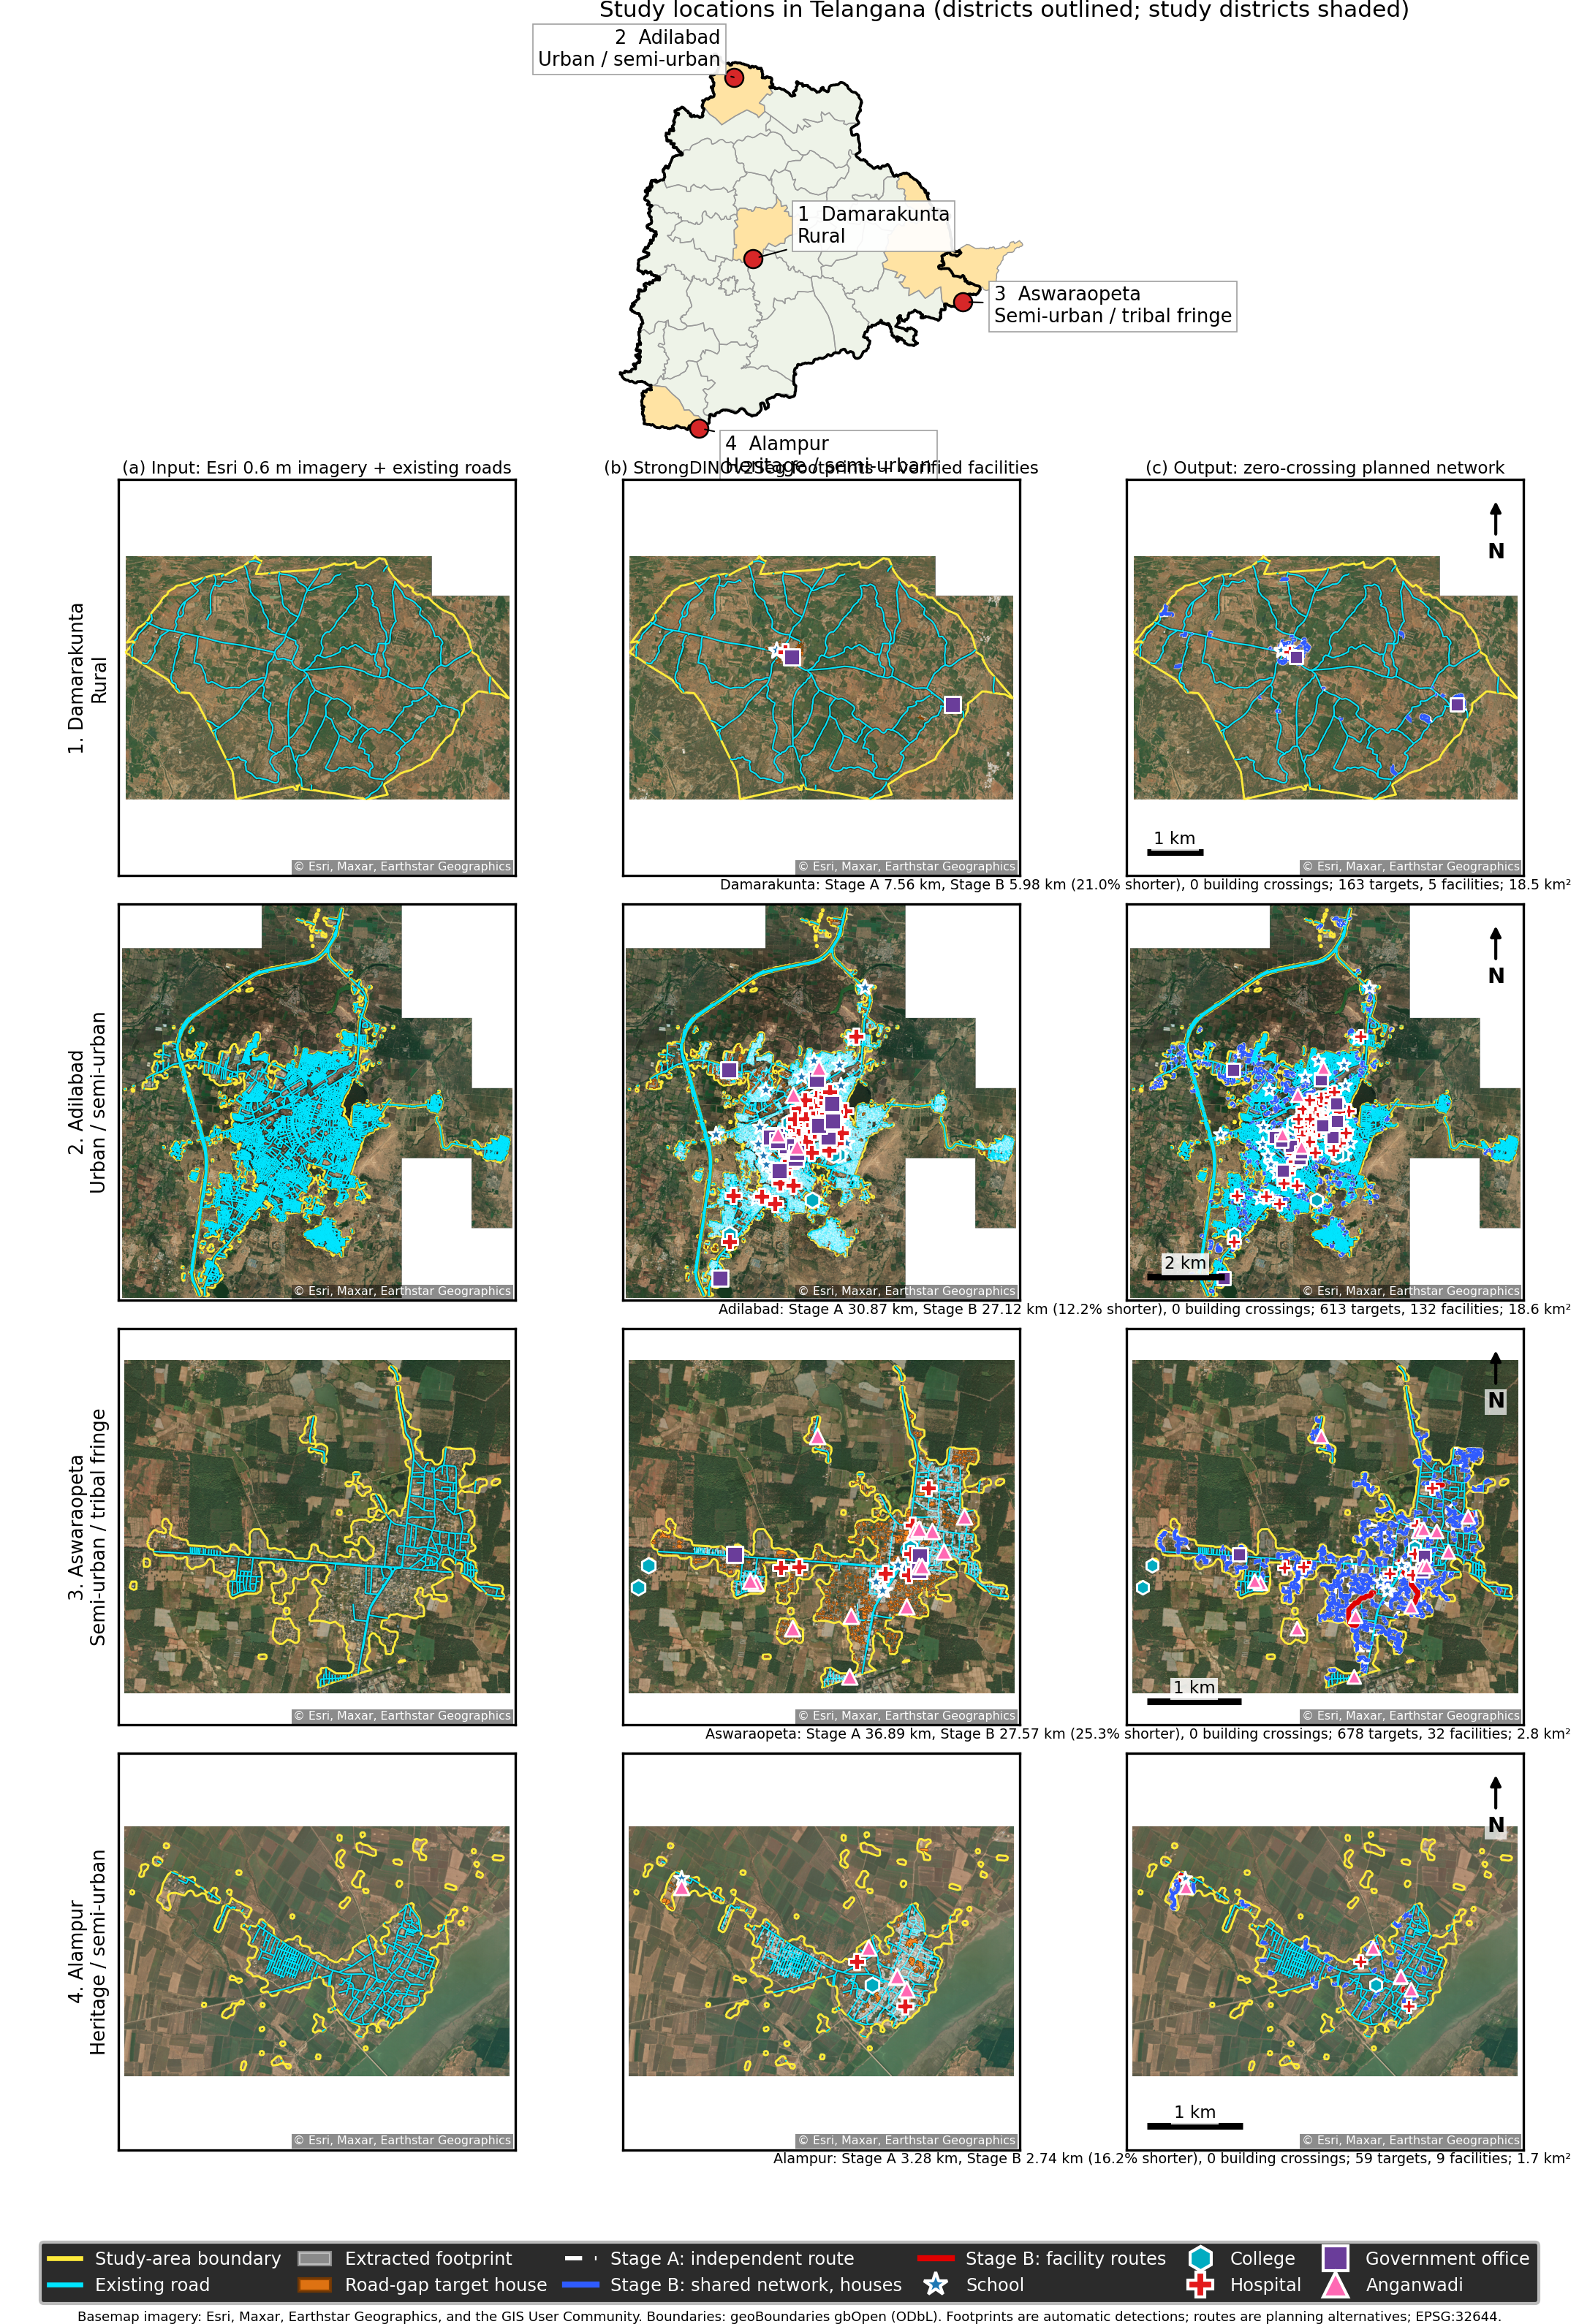
\includegraphics[width=0.93\textwidth]{figures/fig_flow_study_areas.png}}{\fbox{\parbox{0.8\textwidth}{\centering\pending{Figure not generated yet: run \texttt{python scripts/build\_paper\_flow\_figure.py --source segmentation} on the PC that holds the segmentation results.}}}}
\caption{Study areas and end-to-end flow. Top: Telangana with district outlines and the four study locations (1~Damarakunta, rural; 2~Adilabad, urban / semi-urban; 3~Aswaraopeta, semi-urban / tribal fringe; 4~Alampur, heritage / semi-urban). Rows 1--4: (a)~input, Esri World Imagery (0.6~m) with the existing road network; (b)~\dinoseg{} footprints (road-gap target houses in orange) with the verified facilities (School, College, Hospital, Government Office, Anganwadi); (c)~output, existing roads, Stage~A independent routes (white dashed) and Stage~B shared network (blue: houses; red: facilities) with the 5~m zero-crossing clearance, scale bar and north arrow. Basemap imagery: Esri, Maxar, Earthstar Geographics, and the GIS User Community. Footprints are automatic detections and routes are planning alternatives, not engineered roads.}
\label{fig:flow}
\end{figure*}

\begin{table*}[t]
\caption{Four study areas side by side. Segmentation rows: LoveDA validation of the single \dinoseg{} checkpoint (macro averages; F1-score equals the mean Dice). Routing rows: unique lengths on the 5~m zero-crossing grid (Stage~A independent, Stage~B shared network, shared edges once); building crossings are routes inside another building's footprint; the cost is the Stage~B length times Rs 75 lakh per km (range 60--90), an owner-supplied, unverified PMGSY-based rate, so it is illustrative and not an engineering estimate.}
\label{tab:four}
\centering
\scriptsize
\resizebox{\textwidth}{!}{% generated by scripts/run_village_pipeline.py --compare-all (do not edit by hand); \pending{...} marks a value not yet computed on the machine that generated this file
\begin{tabular}{@{}lrrrr@{}}
\toprule
Metric & Damarakunta & Adilabad & Aswaraopeta & Alampur \\
\midrule
\multicolumn{5}{@{}l}{\textit{Study area profile}}\\
District & Siddipet & Adilabad & Bhadradri Kothagudem & Jogulamba Gadwal \\
Typology & Rural & Urban / semi-urban & Semi-urban / tribal fringe & Heritage / semi-urban \\
Window area (km$^2$) & 18.47 & 18.59 & 2.82 & 1.65 \\
Existing road length (km) & 51.7 & 509.9 & 28.6 & 25.3 \\
\midrule
\multicolumn{5}{@{}l}{\textit{Segmentation and extraction (model metrics: LoveDA validation, one checkpoint for all areas)}}\\
Overall accuracy (\%) & \multicolumn{4}{c}{71.3} \\
Precision, macro (\%) & \multicolumn{4}{c}{72.4} \\
Recall, macro (\%) & \multicolumn{4}{c}{66.9} \\
F1-score = mean Dice (\%) & \multicolumn{4}{c}{68.9} \\
mIoU (\%) & \multicolumn{4}{c}{53.8} \\
Extracted building footprints & 165 & 5{,}653 & 1{,}297 & 430 \\
\midrule
\multicolumn{5}{@{}l}{\textit{Verified public infrastructure (audited, on building footprints)}}\\
School & 2 & 39 & 5 & 1 \\
College & 0 & 15 & 3 & 1 \\
Hospital & 1 & 59 & 7 & 2 \\
Government office & 2 & 15 & 3 & 0 \\
Anganwadi & 0 & 4 & 14 & 5 \\
Total verified facilities & 5 & 132 & 32 & 9 \\
\midrule
\multicolumn{5}{@{}l}{\textit{Stage A vs.\ Stage B routing (5\,m zero-crossing clearance) and PMGSY-benchmarked cost}}\\
Road-gap target buildings & 163 & 613 & 678 & 59 \\
Routed buildings & 162 & 607 & 632 & 58 \\
Stage A independent length (km) & 7.56 & 30.87 & 36.89 & 3.28 \\
Stage B shared-trunk length (km) & 5.98 & 27.12 & 27.57 & 2.74 \\
Corridor length saving (\%) & 21.0 & 12.2 & 25.3 & 16.2 \\
Building crossings (routes) & 0 & 0 & 0 & 0 \\
Mean terrain slope (\%) & 3.8 & 3.1 & 3.1 & 2.1 \\
PMGSY-benchmarked cost (INR lakh) & 448 & 2{,}034 & 2{,}067 & 206 \\
\bottomrule
\end{tabular}
% PMGSY-benchmarked cost = unique Stage B length (km) x Rs 75 lakh/km (sensitivity range 60-90)
}
\end{table*}

\section{Discussion}
\subsection{What transfers and what does not}
The planning stages transferred without modification: the same cost surface, solver parameters and metrics produced connected plans in a dense window, both from \dinoseg{} footprints on Esri imagery (345 targets) and from open footprints (874 targets). The qualitative findings were reproduced in all three settings: sharing saves unique length (24.9\%, 14.7\% and 26.0\%), the footprint penalty trades length for exposure, and omissions shorten the plan while stranding households. What did not transfer is the benefit of the simpler baselines: roads-only sharing recovered most of the gain in the dispersed village (22.6\%) but almost none in the dense window (2.3\% and 2.9\%), which suggests that the value of a marginal-cost planner grows with settlement density, a hypothesis supported by one dense window. The two Adilabad footprint sources differ in the size of the saving (14.7\% against 26.0\%); with 57\% of the segmented instances being merged blocks, the segmentation result may reflect coarse, widely spaced targets, and no reference mask exists to say which footprint set is closer to the truth.

\subsection{Why pixel metrics are not enough for infrastructure use}
Segmentation metrics are area-weighted over classes, while the planner counts instances. A detector that misses the smallest quarter of buildings can lose few building pixels yet removes a quarter of households from the plan (table~\ref{tab:omission}), and a detector that merges adjacent roofs can score a high pixel IoU yet strands 38\% of the Damarakunta houses in the merged-blob scenario. Network length falls in both cases, so total length is a poor quality indicator. Merged blobs correspond to dense multi-roof structures; whether they coincide with the core of a hamlet was not measured.

\subsection{Land take and planning use}
Shared corridors reduce the length of new road for the same households. As an illustration only, assuming a 5~m formation width (an assumption of this study; no road-width data were available), the 1{,}684~m saved in Damarakunta corresponds to about 0.84~ha less land take, the 3{,}152~m saved in Adilabad (segmentation targets) to about 1.6~ha and the 12{,}060~m saved against the open-footprint targets to about 6.0~ha. For PMGSY-style schemes \cite{pmgsy} three points follow. Building inventories are uncertain inputs and a network sized from them should carry a sensitivity band. Shared corridors save about a quarter of unique length and this survives omissions. Local overrides should be used sparingly and documented. The outputs are screening-level alternatives; we do not claim compliance with Indian Roads Congress design standards, nor any engineering design value.

\subsection{Limitations}
(i) Two settlements only; the semi-urban and second rural windows are planned but have not been run. (ii) Omission scenarios are synthetic, not measured detection errors. (iii) Neither Damarakunta nor Adilabad has a surveyed reference mask; the LoveDA metrics come from the epoch-4 checkpoint with metadata recovered from the training notebook, and the checkpoint hash (SHA-256 \texttt{2e7c4646dc77ceb2\allowbreak a357f44f11cb3f7f\allowbreak f84e636871d70ba4\allowbreak c31e194e5ec00cf3}) was logged only for the Adilabad run, not with the Damarakunta candidates, although both runs loaded the same file path. (iv) In Adilabad 57\% of the \dinoseg{} instances are \textsc{Unresolved\_Merge} blocks, so its 345 targets are built-up units, not houses; the open footprints are map data of unverified completeness, and Overture licences were not re-verified. Ten of the 68 verified facility points share an identical coordinate with another Overture record (generic geocodes), so the 20 m footprint check is weak evidence in the dense fabric. (v) Costs are ordinal, the planner is a heuristic without an optimality guarantee, and road-gap targeting changes the problem, as the threshold sweep shows. (vi) Pixel accuracy is reported as 71.3\%, the value recomputed from the confusion matrix. (vii) Merged-blob and addition scenarios were run only for Damarakunta.

\section{Conclusions}
A pipeline from satellite imagery and open layers to shared access roads connects the houses and facilities of a rural village (24.9\% less unique corridor than independent routing) and, without changes to the cost surface or solver, those of an urban and peri-urban mandal, end to end on Esri imagery (14.7\% less) and on open footprints (26.0\% less). Footprint penalties and simulated inventory errors behave consistently in all three settings: penalties trade length for fewer routes through dwellings, and omissions shorten the plan while stranding households. The dependence of the roads-only baseline on settlement density, and the effect of detection quality across settings, are the main open questions; a semi-urban and a second rural window are planned to address the first.

\ifanon\else
\section*{Acknowledgments}
The authors acknowledge the Telangana State Remote Sensing Application Centre (TGRAC) for the boundary, road and facility layers of Damarakunta, and the providers of the open datasets used (ESA WorldCover, Copernicus DEM, Overture Maps, geoBoundaries, Google Open Buildings, LoveDA).
\fi

\section*{Data sources and imagery attribution}
High-resolution RGB satellite basemap imagery for Damarakunta Village and the Adilabad Urban window was obtained via Esri World Imagery (sources: Esri, Maxar, Earthstar Geographics, and the GIS User Community) and used strictly for non-commercial academic research and visual overlay in accordance with Esri's academic use terms, while raw imagery tiles are not redistributed. All derived modeling and multi-settlement planning layers rely on open-licensed datasets: ESA WorldCover 10~m v200 (CC BY 4.0), Copernicus GLO-30 DEM (Copernicus Open Access Licence), geoBoundaries ADM3 (ODbL 1.0), and Overture Maps (ODbL 1.0 / CDLA-Permissive-2.0). Damarakunta's boundary, road and facility layers are TGRAC data and its $\sim$30~m DEM source was not recorded; the Copernicus GLO-30 and geoBoundaries layers apply to the Adilabad window.

\section*{Funding}
This research received no specific grant from any funding agency in the public, commercial, or not-for-profit sectors.

\section*{Data availability statement}
\ifanon
Code, derived tables and the open-data manifests (with SHA-256 hashes) will be made available in a public repository on acceptance and are available to reviewers on request. TGRAC layers for Damarakunta are subject to the provider's terms.
\else
Code, derived summary tables, and the open-data manifests with SHA-256 hashes are available at \url{https://github.com/Archana519/Telangana-Rural-Project} (folders \path{DELIVERABLES_DAMARAKUNTA_STAGE_B} and \path{DELIVERABLES_CONTRIBUTION_3_MULTI_VILLAGE}, the latter including the Adilabad segmentation results in \path{01_ADILABAD_SEGMENTATION}). TGRAC layers for Damarakunta are subject to the provider's terms. The \dinoseg{} checkpoint is not included in the repository; its SHA-256 is given in Section~\ref{sec:methods}. A Zenodo DOI will be added when the archive is minted.
\fi

\section*{Conflict of interest}
The authors declare no competing interests.

\bibliographystyle{unsrt}
\bibliography{references}

\end{document}
"      (then bibtex / pdflatex as above)
% The IOP class (iopjournal / iopart) is not installed in this build environment, so the manuscript uses a plain
% `article` layout with the same logical front matter. At submission, paste the sections into the IOP journal
% template (Overleaf: "IOP journal article template", option [anonymous] for double-anonymous review).
% Every number in Sections 3-5 is checked by paper_eris/verify_eris_numbers.py against
% DELIVERABLES_DAMARAKUNTA_STAGE_B/ and DELIVERABLES_CONTRIBUTION_3_MULTI_VILLAGE/01_ADILABAD/.
% =============================================================================================================
\documentclass[12pt,a4paper]{article}
\usepackage[margin=2.5cm]{geometry}
\usepackage{setspace}\onehalfspacing
\usepackage{graphicx}
\usepackage{booktabs}
\usepackage{array}
\usepackage{amsmath,amssymb}
\usepackage{url}
\usepackage{xcolor}
\usepackage{algorithm}
\usepackage{algpseudocode}
\usepackage[hidelinks]{hyperref}
\setlength{\emergencystretch}{3em}
\newif\ifanon
\ifdefined\ANON\anontrue\fi
\newcommand{\dinoseg}{StrongDINOv2Seg}
\newcommand{\Lcost}{L_{\mathrm{cost}}}
\newcommand{\pending}[1]{\textcolor{red}{\textit{#1}}}% value not yet computed on the machine that generated paper_comparison_table.tex
\algrenewcommand\algorithmicrequire{\textbf{Input:}}
\algrenewcommand\algorithmicensure{\textbf{Output:}}

\begin{document}

\begin{center}
{\Large\bfseries Smart village infrastructure planning and road network optimization for rural Telangana\par}
\vspace{0.8em}
\ifanon
{\large [Authors withheld for double-anonymous review]\par}
\else
\small\begin{tabular}{@{}p{0.47\textwidth}p{0.47\textwidth}@{}}
\centering\textbf{Ramakrishna Kolikipogu}\par
\centering\textit{Department of Information Technology}\par
\centering\textit{Chaitanya Bharathi Institute of Technology (A)}\par
\centering Hyderabad, India\par
\centering krkrishna.cse@gmail.com\par
&
\centering\textbf{Pendyala Archana}\par
\centering\textit{Department of Information Technology}\par
\centering\textit{Chaitanya Bharathi Institute of Technology (A)}\par
\centering Hyderabad, India\par
\centering pendyalaarchanareddy98@gmail.com\par
\end{tabular}\\[1.4em]
\fi
\end{center}

\begin{abstract}
\noindent Rural road infrastructure planning faces several challenges, including incomplete spatial data, unplanned settlements, difficult terrain, and limited information about suitable road connections to essential public services such as hospitals, schools, and government institutions. Conventional road-planning approaches often rely on manual decision-making and shortest-path algorithms, which may not adequately consider the influence of spatial-data errors, terrain conditions, land-use constraints, and opportunities for sharing road segments. To address these challenges, this work proposes an AI- and GIS-based framework for rural village infrastructure planning and road-network optimization. The proposed framework integrates high-resolution satellite imagery, existing road-network data, village boundary information, land-cover maps, elevation data, and public-service locations. A StrongDINOv2Seg deep-learning model is employed for semantic segmentation, supported by GIS-based feature extraction to identify relevant spatial features. A multi-criteria cost surface is then generated by considering land-cover conditions, terrain slope, and restricted areas to identify suitable movement paths. For road-network planning, a two-stage approach is implemented: in the first stage, alternative least-cost routes are generated using grid-based Dijkstra pathfinding; in the second stage, a greedy shared-network selection strategy evaluates alternative routes based on their marginal cost and gives credit to road segments already included in the selected network, reducing unnecessary route duplication while prioritizing connections to public-service facilities and residential buildings. The framework is demonstrated on Damarakunta village in Siddipet District, Telangana, and evaluated for cross-morphology transferability in Adilabad Urban. On the LoveDA validation benchmark, the segmentation model achieved a mean Intersection over Union (mIoU) of 53.8\% and a mean Dice score of 68.9\%. In the Damarakunta building-access planning experiment, the two-stage network-aware approach produced 5{,}069.0~m of unique route length compared with 6{,}753.1~m for independent least-cost routing, representing a reduction of 24.9\%. Re-applied end to end to Adilabad Urban on Esri imagery, the same cost surface and solver reduced unique route length from 21{,}440.8~m to 18{,}288.7~m (14.7\%) for 345 road-gap targets, and with open Overture Maps footprints from 46{,}419.2~m to 34{,}358.8~m (26.0\%), confirming consistent network-sharing behavior across contrasting settlement densities, although a roads-only shared reference recovered most of the saving in Damarakunta (22.6\%) but little in Adilabad (2.3\% and 2.9\%). Because most StrongDINOv2Seg instances in Adilabad's dense fabric are merged roof blocks, its targets are built-up units rather than counted houses. The proposed framework provides a GIS-based decision-support approach for analyzing rural infrastructure requirements and generating cost-aware road-network alternatives as computational planning suggestions requiring field validation prior to implementation.
\end{abstract}

\noindent\textit{Keywords}: rural roads, building footprint extraction, satellite remote sensing, least-cost path, shared network, spatial transferability, open geospatial data, Telangana

\section{Introduction}
Road building is among the most consequential land-use changes of the coming decades. Global road length is projected to grow by roughly 3.0--4.7 million km by 2050 \cite{meijer2018global}, and new roads open land to clearing, fragmentation and conversion \cite{laurance2014global}. Much of this growth is local. In India the Pradhan Mantri Gram Sadak Yojana (PMGSY) connects habitations through all-weather rural roads \cite{pmgsy}, and planning for such schemes depends on knowing where dwellings and facilities are, what terrain and land cover a corridor must cross, and which connection rule is applied.

Computational support for this planning has matured along three separate lines. Remote sensing now maps buildings and roads at large scale, from continental building inventories \cite{sirko2021openbuildings} to foundation-model segmenters \cite{oquab2023dinov2}, with recent work addressing small and isolated rural buildings, uncertainty, and domain shift \cite{r62,r63,r64,r65,r66,r67,r68,r69,r70}. Multi-criteria and least-cost analysis translates terrain and land cover into route costs \cite{r06,r53,r54,collischonn2000lcp}. Network-design formulations connect many demand points at low total cost, including Steiner-tree heuristics \cite{kou1981steiner,mehlhorn1988steiner,hwang1992steiner,r51}, rural road design models \cite{r41,r43,r44} and recent analogues for power and transport networks \cite{r45,r46,r47,r50}. These lines are rarely joined: detectors are judged by pixel overlap \cite{r01}, planners assume an error-free inventory, and each house is often connected independently, so neighbouring houses re-trace the same corridor.

We join them in a single reproducible pipeline and test it at two settlement densities. Our contributions are:
\begin{enumerate}
\item \textbf{End-to-end pipeline.} A pipeline from satellite imagery to a shared access network: StrongDINOv2Seg segmentation, OpenCV/NumPy distance-transform instance extraction with an explicit merge flag, a multi-criteria cost surface with a footprint penalty, and a two-stage shared-network planner (Section~\ref{sec:methods}).
\item \textbf{Error propagation.} Controlled omission and addition scenarios that propagate building-inventory errors through the planner, measuring their effect on unique length, coverage and exposure of dwellings (Sections~\ref{sec:damar}--\ref{sec:adilabad}).
\item \textbf{Multi-settlement spatial transferability and open-data scalability.} The rural Damarakunta workflow is re-applied, with the same cost-surface definition and solver, to the Adilabad Urban mandal (urban and peri-urban): end to end on Esri imagery (StrongDINOv2Seg and instance extraction) and, as an independent check, on open Overture Maps footprints, with a road-gap rule for targets and robustness examined over penalty settings, road-gap thresholds and synthetic omissions (Section~\ref{sec:adilabad}).
\end{enumerate}
Two scope limits apply. Only these two settlements were evaluated; a semi-urban and a second rural window are planned but not yet run, so we make no claim about a full rural--semi-urban--urban gradient. And the Adilabad segmentation results are unvalidated: no reference building mask exists, and in the dense fabric most detected instances are merged roof blocks (Section~\ref{sec:adilabad}), so the Adilabad targets are built-up units rather than counted houses.

\section{Related work}
\textbf{Building extraction.} Reviews of building extraction from remote sensing \cite{r01} document the shift from fully convolutional networks \cite{ji2019whu} to transformer and foundation-model encoders. Recent studies target isolated small buildings \cite{r63}, weak supervision \cite{r62}, uncertainty-guided refinement \cite{r64,r65}, and domain generalisation or adaptation across imagery sources \cite{r02,r66,r67,r68,r69,r70}. Road extraction has followed the same path, with width-adaptive, topology-preserving and foundation-model-based networks for rural and arid scenes \cite{r56,r57,r58,r59,r60}, and topological analysis has been used to detect informal settlements worldwide \cite{r48}. Evaluation is overwhelmingly through overlap scores on benchmark data \cite{foody2002status}; the effect of detection errors on downstream infrastructure decisions is rarely quantified, although error propagation in GIS models is long established \cite{heuvelink1998error}.

\textbf{Route and network planning.} Multi-criteria GIS analysis \cite{r06} and least-cost path methods \cite{collischonn2000lcp,r53,r54} underlie corridor selection for roads, with dedicated treatments of slope \cite{r54}, route alternatives \cite{r53} and travel-time uncertainty \cite{r61}, and GIS route reconstruction has been applied to historical transport routes \cite{r55}. Rural road design has been addressed with improved network-design models \cite{r41}, algorithmic planning under constrained capacities in India \cite{r43} and facility-based methodology \cite{r44}. Steiner-tree formulations \cite{hwang1992steiner} and their shortest-path-based heuristics \cite{kou1981steiner,mehlhorn1988steiner} connect many terminals at low total length and are applied to sub-network identification \cite{r51}, multi-terminal routing \cite{r52}, cable routing \cite{r45}, minimum spanning trees of road networks \cite{r46}, rural grids \cite{r47} and least-cost electrification \cite{r50}.

\textbf{Gap.} To our knowledge no cited work combines (i) satellite-derived building instances, (ii) a land-cover- and slope-based cost surface with building avoidance, (iii) a shared-network planner whose marginal cost credits built corridors, and (iv) a systematic test of how inventory omissions and the settlement setting change the result. This paper addresses that combination for rural Telangana and treats the comparison between two settlements as an explicit transferability test.

\section{Study areas and data}
\subsection{Damarakunta (rural)}
Damarakunta is a rural revenue village in Markook mandal, Siddipet district, Telangana ($\approx 17.707^{\circ}$N, $78.753^{\circ}$E). Its boundary, from the Telangana State Remote Sensing Application Centre (TGRAC), encloses 18.47~km$^2$ (UTM zone 44N, EPSG:32644; figure~\ref{fig:flow}). Settlement is dispersed, with small house clusters separated by farmland. A 0.6~m, three-band mosaic (11{,}296 $\times$ 7{,}171 px) was assembled from Esri World Imagery exports. Building candidates are model outputs: 278 polygons, 165 inside the boundary, of which 163 are used as routing targets. They carry a quality class: \textsc{Plausible} (71), \textsc{Review} (32) and \textsc{Unresolved\_Merge} (62), the last denoting blobs that merge adjacent roofs and could not be split. Five TGRAC facilities (schools, a health sub-centre and the gram-panchayat headquarters points) are planned in a separate phase. No ground-truth building mask exists for Damarakunta.

\subsection{Adilabad Urban (urban and peri-urban)}\label{sec:adilabad_data}
The second window is the Adilabad Urban mandal, Adilabad district (geoBoundaries ADM3 polygon; centroid $19.682^{\circ}$N, $78.528^{\circ}$E), 17.75~km$^2$, close to Damarakunta in area. The 10~m grid has 424 $\times$ 564 cells, 177{,}533 of them inside the polygon, 0.62\% blocked (water or slope $>25^{\circ}$). About 60\% of cells are not WorldCover built-up, so the window holds an urban core and a peri-urban fringe. The boundary layer is the 2018 release and may differ from current municipal limits.

Two sets of building footprints are used. (i)~\emph{Segmentation footprints (primary, end to end).} A 0.6~m Esri World Imagery mosaic of the window (7{,}248 $\times$ 9{,}590~px, EPSG:32644) was exported with the Damarakunta recipe (1{,}800~m tiles). \dinoseg{} was applied to 391 tiles of $560\times560$~px (stride 420~px, margin 70~px, the Damarakunta tiling; Damarakunta: 459 tiles) and the same instance extraction. This yields 2{,}769 instances, of which 2{,}690 have an area of at least 30~m$^2$ and form the penalty layer; their quality classes are \textsc{Plausible} (1{,}033), \textsc{Review} (77) and \textsc{Unresolved\_Merge} (1{,}580), the last with a median area of 1{,}125.5~m$^2$ (\textsc{Plausible}: 207.4~m$^2$). Of 83 Overture place candidates inside the window, 68 are verified with the Damarakunta rule (a detected footprint within 20~m): 44 schools, 20 health and 4 government. (ii)~\emph{Open footprints (independent check).} Overture release 2026-10-21.0 \cite{overture2026} supplies 4{,}850 road segments, 24{,}924 building polygons (18{,}846 from OpenStreetMap, 6{,}078 from Google Open Buildings v3 \cite{sirko2021openbuildings}) and 738 places; footprints with area $\ge 30$~m$^2$ and confidence $\ge 0.7$ (18{,}242 polygons) form the penalty layer, and 71 of the 83 facility candidates are verified (44 schools, 20 health, 7 government) after manual removal of mis-geocoded records. Roads are Overture/OSM segments in both variants (table~\ref{tab:data}). Neither footprint set has been field-verified. Figure~\ref{fig:flow} shows the study window, the detected footprints and the verified facilities of every study area.

\begin{table}[t]
\caption{Input data and licence status. ``Not re-verified'' marks Overture licences taken from the provider documentation, which could not be opened from the execution environment.}
\label{tab:data}
\centering
\footnotesize
\begin{tabular}{@{}>{\raggedright\arraybackslash}p{3.0cm}>{\raggedright\arraybackslash}p{5.9cm}>{\raggedright\arraybackslash}p{5.5cm}@{}}
\toprule
Layer & Damarakunta / Adilabad source & Licence status \\
\midrule
Boundary & TGRAC polygon / geoBoundaries ADM3 \cite{runfola2020geoboundaries} & TGRAC: not stated / ODbL 1.0 \\
Roads, facilities & TGRAC (43 road features, 5 facilities) / Overture Maps 2026-10-21.0 \cite{overture2026} & TGRAC: not stated / ODbL 1.0 (roads), CDLA-Permissive-2.0 (places); not re-verified \\
Buildings & StrongDINOv2Seg instances (0.6~m Esri imagery; both windows) / Overture footprints (Adilabad check; OSM, Google Open Buildings v3 \cite{sirko2021openbuildings}) & Esri academic-use terms, tiles not redistributed / ODbL 1.0 and CC BY 4.0; not re-verified \\
Land cover & ESA WorldCover v200, 10~m \cite{zanaga2021worldcover} & CC BY 4.0 \\
Terrain & $\sim$30~m DEM (source not recorded) / Copernicus GLO-30 \cite{esa2022copdem}; Sobel slope, bilinear to 10~m & Not stated / Copernicus Open Access Licence \\
Training benchmark & LoveDA \cite{wang2021loveda} & Source domain only \\
\bottomrule
\end{tabular}
\end{table}

\section{Methods}\label{sec:methods}
The framework is a seven-step chain (figure~\ref{fig:arch}): (1)~multi-source open-data ingestion (Esri World Imagery, ESA WorldCover, Copernicus GLO-30, Overture / OSM / TGRAC roads, the study polygon); (2)~\dinoseg{} semantic segmentation in 560~px tiles; (3)~distance-transform extraction of building footprints and road-gap targets; (4)~a four-pass multi-source facility audit that snaps every facility onto a roof; (5)~a multi-criteria cost surface with a 5~m zero-crossing building clearance; (6)~Stage~A and Stage~B Dijkstra shared-network routing; and (7)~connectivity and PMGSY-based cost evaluation. Steps 1 to 7 are identical for all four study areas; the settlements differ only in their inputs. The ten-metre soft-penalty planner of the earlier experiments is kept as a comparison baseline (section~\ref{sec:damar}), and the clearance network is the proposed plan (section~\ref{sec:four}).

\begin{figure}[t]
\centering
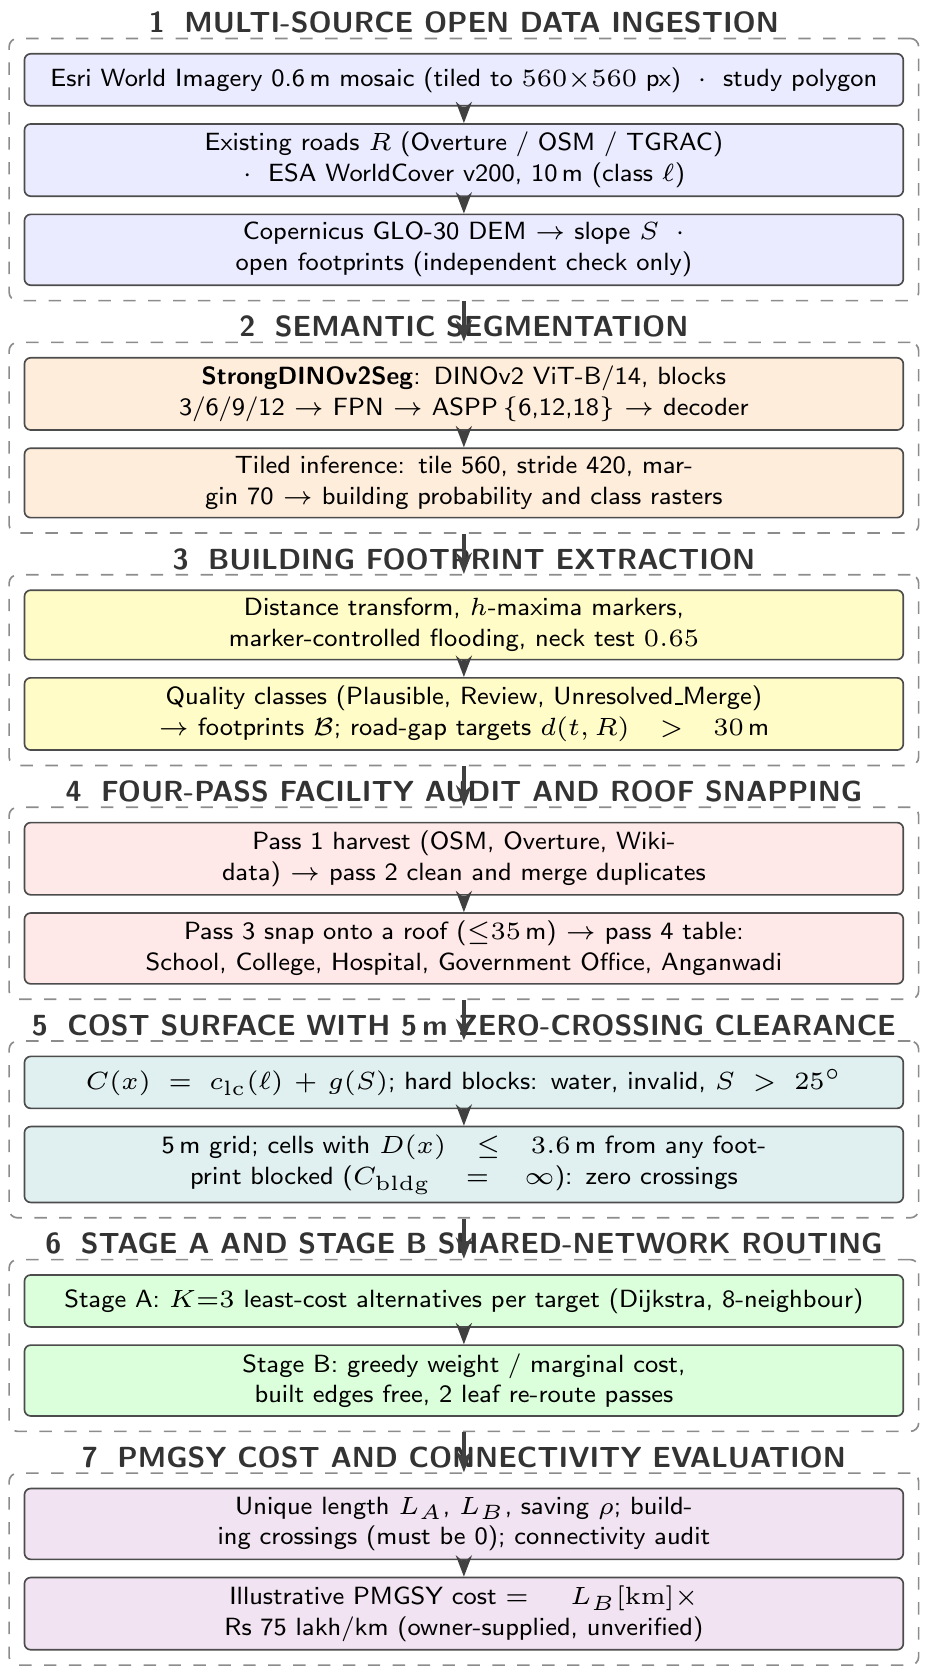
\includegraphics[width=0.5\textwidth]{figures/fig_architecture.png}
\caption{Seven-step architecture: (1)~multi-source open-data ingestion, (2)~\dinoseg{} semantic segmentation (tile 560, stride 420, margin 70), (3)~distance-transform building footprint extraction (neck ratio 0.65), (4)~four-pass multi-source facility audit and roof snapping (School, College, Hospital, Government Office, Anganwadi), (5)~cost surface with a 5~m zero-crossing clearance (3.6~m), (6)~Stage~A independent and Stage~B shared-network Dijkstra routing, (7)~PMGSY cost and connectivity evaluation.}
\label{fig:arch}
\end{figure}

\subsection{Building extraction}
\dinoseg{} is a fully fine-tuned DINOv2 ViT-B/14 encoder \cite{oquab2023dinov2}. Tokens from blocks 3, 6, 9 and 12 are projected to 256 channels, fused (FPN-style \cite{lin2017fpn}), passed through an ASPP neck (rates 6, 12, 18) \cite{chen2018deeplabv3plus} and a four-stage decoder with auxiliary heads for deep supervision \cite{lee2015dsn}. Training used LoveDA \cite{wang2021loveda} at 560~px for a scheduled 10 epochs (AdamW, cosine schedule to $10^{-7}$, encoder learning rate $\times 0.1$) with loss $0.5\,\mathrm{CE}+0.4\,\mathrm{Dice}+0.1\,\mathrm{edge}$ \cite{milletari2016vnet} and auxiliary weight 0.4. The epoch-4 checkpoint was used; the file used for the Adilabad run has SHA-256 \texttt{2e7c4646dc77ceb2\allowbreak a357f44f11cb3f7f\allowbreak f84e636871d70ba4\allowbreak c31e194e5ec00cf3}. Building instances are extracted from the predicted mask with OpenCV and NumPy: h-maxima of the distance transform give markers, a neck test (ratio 0.65) decides whether touching blobs are split, and blobs that cannot be split are flagged \textsc{Unresolved\_Merge}.

\subsection{Road-gap targets and Adilabad footprint sources}
For Adilabad the same imagery-to-footprint chain is run on Esri imagery (Section~\ref{sec:adilabad_data}), and Overture footprints serve as an independent check. Because connecting every footprint is meaningless in a built-up fabric already served by roads, only houses more than 30~m (the planner snap distance) from an existing road are routed. Planner cost grows roughly quadratically with the number of targets, which further motivates the filter; the threshold is varied (20, 30, 50~m) in Section~\ref{sec:adilabad}.

\subsection{Cost surface}
Let $\mathcal{B}$ be blocked cells (water, invalid cells, slope $>25^{\circ}$) and $\mathcal{P}$ the cells whose centre lies inside a footprint. The graph has the unblocked 10~m cells as nodes and 8-neighbour edges with no diagonal corner-cutting. The cell cost is
\begin{equation}
c(x)=\bigl[c_{\mathrm{lc}}(\ell(x))+g(s(x))\bigr]\,m(x),\qquad m(x)=\begin{cases}\mu & x\in\mathcal{P}\\ 1 & \text{otherwise,}\end{cases}
\label{eq:cell}
\end{equation}
where $\ell$ is the WorldCover class with resistance $c_{\mathrm{lc}}=8,5,3,6,2,4$ for trees, shrubland, grassland, cropland, built-up and bare/sparse land respectively (classes 10--60 in the order 10, 20, 30, 40, 50, 60), $g(s)=4\,\mathrm{clip}(s,0,10)/10$ with $s$ the slope in degrees, and $\mu=4$ is the footprint penalty. Edge weights are the mean end-cell cost times step length. Costs are ordinal planning units, not currency. In Damarakunta the penalty is lifted within a 20~m disc around the health sub-centre,  The land-cover, slope, cost and blocked-cell rasters are the inputs of the cost surface of every study area (figure~\ref{fig:flow}).whose point lies on the edge of its own footprint.

\subsection{Shared-network planner}
For each target, Stage~A computes a least-cost path to the existing road cells with Dijkstra's algorithm \cite{dijkstra1959note,hart1968astar,collischonn2000lcp} and alternatives by inflating costs along earlier paths ($K=3$ alternatives in total). Stage~B greedily selects the (target, alternative) pair with the highest weight per marginal cost
\begin{equation}
\Delta\Lcost\bigl(\pi\mid S\bigr)=\sum_{e\in\pi\setminus E_S}w(e),
\label{eq:marginal}
\end{equation}
where $E_S$ is the set of already selected edges, so built edges are free and a route may end on another route. This is the shortest-path heuristic for Steiner trees \cite{kou1981steiner,mehlhorn1988steiner} on a penalised, land-cover-weighted graph with the road network as a free sub-tree; it carries no optimality guarantee. Two passes of leaf re-routing follow. Snap distance is 30~m, search limit 1{,}500~m and attachment tolerance 15~m. Facilities are planned in a separate phase.

\subsection{Facility audit and roof snapping}
Overture Places alone mislocated or missed colleges, hospitals, offices and anganwadis, so the facilities of each area come from a four-pass audit (\texttt{scripts/audit\_facilities.py}). Pass~1 harvests candidates inside and within 500~m of the polygon from OpenStreetMap (Overpass and the Photon geocoder), Overture Places, Wikidata and Wikipedia (and, for Damarakunta, the TGRAC layers); LGD, UDISE+ and the district directories have no open query interface and were not used. Pass~2 assigns one of five categories (School, College, Hospital, Government Office, Anganwadi), removes closed or commercial records (pharmacies, laboratories, coaching centres, banks, cooperative societies), religious sites, foreign place names, placeholder coordinates shared by several differently named records, and merges duplicates of one campus across sources; every removal is logged with its reason. Pass~3 moves each survivor onto the footprint that contains it or, failing that, the nearest footprint of at least 25~m$^2$ within 35~m (a compound building up to 25~m away for a school, college or hospital), and removes facilities with no building in range. Pass~4 writes the verified table with the sources, the snap distance and a confidence label; records with a single source and a snap of more than 12~m are kept with \texttt{use\_in\_analysis}${}=$\,False and are not routed.

\subsection{Zero-crossing building clearance}
The soft footprint penalty $\mu$ in equation~\ref{eq:cell} lets a route cross a roof when the detour costs more. The proposed plan therefore uses a hard barrier on a finer grid. Each 10~m cost cell is refined to $2\times2$ cells of cell size $\Delta=5$~m with the same cost per metre, and every cell whose centre lies within $r_c=3.6$~m of any footprint is blocked (equation~\ref{eq:bldg}). Because $r_c>\Delta\sqrt2/2=3.54$~m, no step between two free cell centres can touch a footprint: a point of the step lies within $\Delta\sqrt2/2$ of one of its end points, and that end point would then have been blocked. A target sits inside its own building, so each route starts at the edge of that building and reaches the nearest free cell that is connected to the road network by a straight lane of at most the snap distance that touches no other footprint; a target with no such lane (a house enclosed by other buildings) is reported as unrouted, never routed over a roof. Lengths are measured from the building edge. Every drawn route (lane, path and attachment to a road) is finally intersected with all footprints other than its own.

\subsection{Mathematical formulation}
\paragraph{Segmentation loss.} With logits $\mathbf z$, labels $y$, class probabilities $p_{ic}$ and one-hot targets $t_{ic}$ at pixel $i$ (class 0 is ignored),
\begin{equation}
\mathcal L(\mathbf z,y)=0.5\,\mathcal L_{\mathrm{CE}}+0.4\,\mathcal L_{\mathrm{Dice}}+0.1\,\mathcal L_{\mathrm{edge}},\qquad
\mathcal L_{\mathrm{total}}=\mathcal L(\mathbf z^{\mathrm{main}},y)+0.4\sum_{j=1}^{3}\mathcal L(\mathbf z^{(j)},y),
\label{eq:loss}
\end{equation}
\begin{equation}
\mathcal L_{\mathrm{Dice}}=\frac1{|\mathcal C|}\sum_{c\in\mathcal C}\Bigl(1-\frac{2\sum_i p_{ic}t_{ic}+\varepsilon}{\sum_i p_{ic}+\sum_i t_{ic}+\varepsilon}\Bigr),\qquad
\mathcal L_{\mathrm{edge}}=\frac1{|\Omega|}\sum_{i\in\Omega}(1+4e_i)\,\mathrm{CE}_i,\quad e_i=\min\{1,\,|(K_x{*}y)_i|+|(K_y{*}y)_i|\}.
\label{eq:diceedge}
\end{equation}
Here $\mathcal C$ is the set of scored classes, $\varepsilon$ a small smoothing constant, $K_x,K_y$ the Sobel kernels, so that the edge term up-weights the cross-entropy of pixels on label boundaries by up to five; the three auxiliary heads $\mathbf z^{(j)}$ provide deep supervision.

\paragraph{Evaluation metrics.} From the confusion matrix, with $TP_c,FP_c,FN_c$ the true positives, false positives and false negatives of class $c$ and $N$ the number of labelled pixels,
\begin{equation}
\mathrm{OA}=\frac{\sum_c TP_c}{N},\quad P_c=\frac{TP_c}{TP_c+FP_c},\quad R_c=\frac{TP_c}{TP_c+FN_c},\quad F_{1,c}=\frac{2P_cR_c}{P_c+R_c}=\frac{2TP_c}{2TP_c+FP_c+FN_c},\quad \mathrm{IoU}_c=\frac{TP_c}{TP_c+FP_c+FN_c},
\label{eq:metrics}
\end{equation}
and $P$, $R$, $F_1$ (the Dice coefficient) and $\mathrm{mIoU}=|\mathcal C|^{-1}\sum_{c\in\mathcal C}\mathrm{IoU}_c$ are the macro averages over the scored classes. Because $F_{1,c}$ equals the per-class Dice score, the reported F1-score is the mean Dice.

\paragraph{Terrain.} Slope is taken from the Copernicus GLO-30 elevation $z$ with the Sobel gradient at the DEM spacing $\Delta_z=30$~m, resampled bilinearly to the planning grid:
\begin{equation}
\partial_x z\approx\frac{(K_x{*}z)}{8\Delta_z},\quad \partial_y z\approx-\frac{(K_y{*}z)}{8\Delta_z},\quad S=\arctan\sqrt{(\partial_x z)^2+(\partial_y z)^2},\quad p_S=100\tan S,
\label{eq:slope}
\end{equation}
with $S$ the slope in degrees and $p_S$ the equivalent percentage slope reported in the comparison table. The cost uses the linear ramp $g(S)=w_s\min(S,S_{\mathrm{ref}})/S_{\mathrm{ref}}$ with $w_s=4$ and $S_{\mathrm{ref}}=10^{\circ}$, and cells with $S>S_{\lim}=25^{\circ}$ are blocked; no separate IRC slope-penalty factor is applied.

\paragraph{Composite cost and clearance barrier.} With $c_{\mathrm{lc}}(\ell)$ the WorldCover resistance (equation~\ref{eq:cell}, so the land-cover weight is $w_{\mathrm{lc}}=1$) and $D(x)$ the Euclidean distance from the centre of cell $x$ to the nearest footprint (zero inside a footprint),
\begin{equation}
C(x)=c_{\mathrm{lc}}(\ell(x))+g(S(x))+C_{\mathrm{bldg}}(x),\qquad C_{\mathrm{bldg}}(x)=\begin{cases}\infty & D(x)\le r_c\\ 0 & \text{otherwise,}\end{cases}\qquad r_c=3.6\ \mathrm{m},\ \Delta=5\ \mathrm{m}.
\label{eq:bldg}
\end{equation}
The ten-metre comparison baseline instead multiplies the cost of cells whose centre lies in a footprint by $\mu=4$ (equation~\ref{eq:cell}).

\paragraph{Graph and routing objectives.} The graph has the free cells as nodes and 8-neighbour edges, a diagonal step being allowed only if both orthogonal neighbours are free. The weight of an edge $(u,v)$ is
\begin{equation}
w(u,v)=d(u,v)\,\frac{C(u)+C(v)}{2},\qquad d(u,v)=\begin{cases}\Delta&\text{cardinal step}\\ \sqrt2\,\Delta&\text{diagonal step.}\end{cases}
\label{eq:edge}
\end{equation}
Stage~A gives every target $t$ the independent least-cost path $\pi_t^{A}=\arg\min_{\pi:\,t\to R}\sum_{e\in\pi}w(e)$ to the existing road cells $R$ (Dijkstra), and two further alternatives that multiply $w(e)$ by $\lambda\in\{3,8\}$ on cells within $20$~m of the earlier paths and overlap them by at most 80\%. Stage~B starts from $E_S=\emptyset$ and repeatedly serves the target and route with the highest weight per marginal cost,
\begin{equation}
(t^\star,\pi^\star)=\arg\max_{t\in U,\ \pi\in\Pi_t\cup\{\pi_t^{\mathrm{net}}\}}\frac{\omega_t}{\Delta\Lcost(\pi\mid S)},\qquad
\Delta\Lcost(\pi\mid S)=\sum_{e\in\pi\setminus E_S}w(e),
\label{eq:stageb}
\end{equation}
where $U$ is the set of unserved targets, $\Pi_t$ the Stage~A alternatives, $\pi_t^{\mathrm{net}}$ the least-cost path to the roads together with the routes already selected, and $\omega_t$ the priority weight ($4$ for hospitals and health centres, $3$ for schools, colleges and anganwadis, $2$ for government offices, $1$ for houses). A built edge $e\in E_S$ thus costs nothing again, which is a discount factor $\alpha=0$ on $E_S$; no intermediate $\alpha\in(0,1)$ is used. With $L(\cdot)$ the total length of the unique edges of a route set (shared edges once),
\begin{equation}
\rho=\frac{L_A-L_B}{L_A}\times100\%,\qquad L_A=L\bigl(\{\pi_t^A\}\bigr),\quad L_B=L(E_S),\qquad X=\sum_{r}\Bigl|r\cap\bigcup_{b\ne b_r}b\Bigr|=0,
\label{eq:saving}
\end{equation}
where $X$ is the length of routes inside footprints other than the route's own building $b_r$ (zero by construction under equation~\ref{eq:bldg}).

\paragraph{Illustrative cost.} The capital cost is
\begin{equation}
\mathrm{Cost}_{\mathrm{INR\ lakh}}=L_B[\mathrm{km}]\times c_{\mathrm{PMGSY}},\qquad c_{\mathrm{PMGSY}}=75\ \text{lakh/km}\ (\text{range }60\text{--}90),
\label{eq:cost}
\end{equation}
with 1 lakh $=10^{5}$~INR. The rate was supplied by the project owner as PMGSY-based and has not been verified against a PMGSY document or a State Schedule of Rates, so the cost is illustrative and not an engineering estimate.

\subsection{Algorithms}
\begin{algorithm}[t]
\caption{Tiled \dinoseg{} inference and distance-transform building extraction (\texttt{run\_tiled\_inference.py}, \texttt{extract\_buildings\_v8.py})}
\label{alg:extract}
\begin{algorithmic}[1]
\Require mosaic $I$ (0.6~m), checkpoint $\theta$, tile $T=560$, stride $s=420$, margin $m=70$, neck ratio $\eta=0.65$, seed height $h=0.3$~m
\Ensure footprints $\mathcal B$ with quality classes
\State \textbf{assert} $s\le T-2m$ \Comment{no gaps between tile centres}
\For{each tile of size $T\times T$ at stride $s$}
  \State $p\gets\mathrm{softmax}(f_\theta(\text{tile}))$; write class $\arg\max p$ and $p_{\mathrm{bldg}}$ for the tile centre (drop $m$ px at inner edges)
\EndFor
\State $M\gets(\text{class}=\text{building})\wedge\lnot\text{no-data}$; drop components smaller than 6~m$^2$
\For{each connected component $K$ of $M$}
  \State $D\gets\mathrm{EDT}(K)$ (smoothed, $\sigma=1$ px); markers $\gets$ $h$-maxima of $D$ with height $h$
  \State pieces $\gets$ marker-controlled flooding of $-D$ (only if area $\ge 40$~m$^2$)
  \For{each adjacent piece pair $(a,b)$}
    \State $r_{ab}\gets D_{\mathrm{saddle}}/\min(D_a^{\max},D_b^{\max})$
    \If{$r_{ab}>\eta$ \textbf{or} a piece is smaller than 12~m$^2$} merge $a,b$ \Comment{no real neck}
    \EndIf
  \EndFor
\EndFor
\State polygonise; flag \textsc{Unresolved\_Merge} if area $>4\times$ the median compact roof; assign \textsc{Plausible} / \textsc{Review} / \textsc{Small} by confidence and shape
\State \Return $\mathcal B$
\end{algorithmic}
\end{algorithm}

\begin{algorithm}[t]
\caption{Cost surface with zero-crossing clearance and two-stage routing (\texttt{clearance.py}, \texttt{plan\_network\_v2.py})}
\label{alg:route}
\begin{algorithmic}[1]
\Require land cover $\ell$, DEM $z$, roads $R$, footprints $\mathcal B$, targets $\mathcal T$ (road-gap houses and verified facilities with weights $\omega_t$), $\Delta=5$~m, $r_c=3.6$~m, $K=3$
\Ensure route sets $\{\pi_t^A\}$, $E_S$ and lengths $L_A$, $L_B$, saving $\rho$, cost
\State $S\gets$ slope of $z$ (equation~\ref{eq:slope}); $C_0(x)\gets c_{\mathrm{lc}}(\ell(x))+g(S(x))$; block water, invalid cells and $S>25^{\circ}$
\State refine $C_0$ from 10~m to $\Delta=5$~m (same cost per metre); $D\gets\mathrm{EDT}(\mathcal B)$; $C(x)\gets\infty$ where $D(x)\le r_c$
\State keep the free cells connected to a road cell; edge weights $w$ by equation~\ref{eq:edge}
\For{each target $t\in\mathcal T$}
  \State entrance $e_t\gets$ point of the target's building edge nearest to a free cell $s_t$; require a lane $e_t\to s_t$ of at most 30~m that touches no other footprint, else mark $t$ unrouted
  \State $\Pi_t\gets K$ Dijkstra alternatives from $s_t$ to $R$ (corridor inflation $\lambda\in\{3,8\}$, 20~m, overlap $\le 80\%$); $\pi_t^A\gets$ first alternative
\EndFor
\State $L_A\gets L(\{\pi_t^A\})$; $U\gets$ routed targets; $E_S\gets\emptyset$
\While{$U\ne\emptyset$}
  \For{each $t\in U$} add the least-cost path $\pi_t^{\mathrm{net}}$ to $R\cup E_S$ to the candidates $\Pi_t$ \EndFor
  \State $(t^\star,\pi^\star)\gets\arg\max\ \omega_t/\Delta\Lcost(\pi\mid S)$ (equation~\ref{eq:stageb}); $E_S\gets E_S\cup\pi^\star$; $U\gets U\setminus\{t^\star\}$
\EndWhile
\State two leaf re-route passes: replace a route that no other route uses if it has become cheaper given the others
\State verify $X=0$ (equation~\ref{eq:saving}); $L_B\gets L(E_S)$; $\rho\gets 100(L_A-L_B)/L_A$; cost by equation~\ref{eq:cost}
\end{algorithmic}
\end{algorithm}

\subsection{Baselines, scenarios and metrics}
Four baselines are compared: straight lines, independent least-cost routes, a length-only control (cost surface replaced by distance) and a roads-only shared reference (routes may share edges only with the existing road network). The saving against independent routing is $\rho=(L_{\mathrm{ind}}-L)/L_{\mathrm{ind}}$, with $L$ the unique network length (shared edges counted once). The exposure metrics are the number of routes crossing another house's footprint and the route length inside other footprints. The footprint penalty is varied ($\mu\in\{1,4,20,100\}$, with a variant in which footprints are buffered by 7.1~m). For omissions, a target set $M$ is removed from the targets and from the penalty layer (a missed detection is absent from both), and the planner is re-run; random draws use seeds 1--5. Coverage, unserved households, change in unique length and length per routed target are reported.

\section{Results: Damarakunta}\label{sec:damar}
\subsection{Detection}
On the 1{,}669-image LoveDA validation split (560~px, seven scored classes) the epoch-4 checkpoint reached 53.8\% mIoU, 68.9\% Dice and 71.3\% pixel accuracy, with 72.4\% macro precision and 66.9\% macro recall; for the Building class IoU is 54.0\%, precision 62.1\% and recall 80.6\% (table~\ref{tab:seg}). These are source-domain figures, not accuracy on Damarakunta. Against Google Open Buildings v3 as a proxy (not ground truth), 118 of the 165 in-boundary candidates agree (71.5\%).

\begin{table}[t]
\caption{Detection evaluation. Top: LoveDA validation (source domain); precision and recall are macro-averages over the seven scored classes. Bottom: agreement of the 165 Damarakunta candidates with Open Buildings v3 (a proxy, not accuracy).}
\label{tab:seg}
\centering
\small
\begin{tabular}{@{}lrrrrr@{}}
\toprule
\multicolumn{6}{@{}l}{\textit{LoveDA validation split (\%)}}\\
 & mIoU & Dice & Pixel acc. & Precision & Recall\\
\midrule
StrongDINOv2Seg & 53.8 & 68.9 & 71.3 & 72.4 & 66.9\\
\quad Building class & 54.0 & 70.1 & --- & 62.1 & 80.6\\
\midrule
\multicolumn{6}{@{}l}{\textit{Damarakunta candidates vs.\ Open Buildings v3}}\\
Class & Candidates & Agree & Disagree & \multicolumn{2}{c}{Agreement (\%)}\\
\midrule
All & 165 & 118 & 47 & \multicolumn{2}{c}{71.5}\\
\textsc{Plausible} & 71 & 51 & 20 & \multicolumn{2}{c}{71.8}\\
\textsc{Review} & 32 & 14 & 18 & \multicolumn{2}{c}{43.8}\\
\textsc{Unresolved\_Merge} & 62 & 53 & 9 & \multicolumn{2}{c}{85.5}\\
\bottomrule
\end{tabular}
\end{table}

\subsection{Shared network and footprint penalty}
Independent least-cost routes for the 163 houses total 10{,}045~m, but because neighbouring houses re-trace the same corridors the unique built length is 6{,}753~m (table~\ref{tab:routing}, figure~\ref{fig:routing}a). The two-stage plan reduces this to 5{,}069~m, a saving of 24.9\%; all 163 houses and five facilities are connected. The length-only control is 3.4\% \emph{longer} in unique length than independent cost-surface routing, and the roads-only shared reference saves 22.6\%, so most of the saving comes from sharing and a further 2.3 percentage points from sharing between new routes.

The penalty trades length for exposure (figure~\ref{fig:routing}b). With $\mu=1$ the plan is shortest (4{,}705~m) but 56 routes pass through other houses (660~m inside footprints). With $\mu=4$ it is 7.7\% longer while crossings halve to 28 routes and 209~m. Buffering footprints by 7.1~m with $\mu=20$ or 100 lowers crossings further (19 routes) at 6{,}190--6{,}238~m.

\begin{table}[t]
\caption{Damarakunta routing, 163 houses ($\mu=4$ unless stated). Total length counts every route; unique length counts shared edges once; $\rho$ is the saving in unique length against independent routes.}
\label{tab:routing}
\centering
\footnotesize
\begin{tabular}{@{}>{\raggedright\arraybackslash}p{4.3cm}rrrrr@{}}
\toprule
Strategy & Total (m) & Unique (m) & $\rho$ (\%) & Routes crossing & In footprints (m)\\
\midrule
Straight line (2 targets infeasible) & 8{,}092.3 & --- & --- & 60 & 1{,}453.2\\
Independent least-cost routes & 10{,}045.4 & 6{,}753.1 & 0.0 & 46 & 328.3\\
Length-only control & 9{,}166.3 & 6{,}979.8 & $-3.4$ & 64 & 1{,}615.8\\
Roads-only shared reference & 5{,}229.3 & 5{,}229.3 & 22.6 & 29 & 216.1\\
\textbf{Two-stage plan (proposed)} & \textbf{5{,}069.0} & \textbf{5{,}069.0} & \textbf{24.9} & \textbf{28} & \textbf{209.1}\\
\midrule
\multicolumn{6}{@{}l}{\textit{No footprint penalty ($\mu=1$)}}\\
Independent least-cost routes & 9{,}595.9 & 6{,}921.3 & 0.0 & 63 & 1{,}423.1\\
Two-stage plan & 4{,}705.5 & 4{,}705.4 & 32.0 & 56 & 660.1\\
\midrule
\multicolumn{6}{@{}l}{\textit{Buffered footprints (7.1~m), two-stage plan}}\\
Penalty $\mu=20$ & --- & 6{,}238.1 & 18.5 & 19 & 147.9\\
Penalty $\mu=100$ & --- & 6{,}190.3 & 18.9 & 19 & 144.8\\
\bottomrule
\end{tabular}
\end{table}

\begin{figure}[t]
\centering
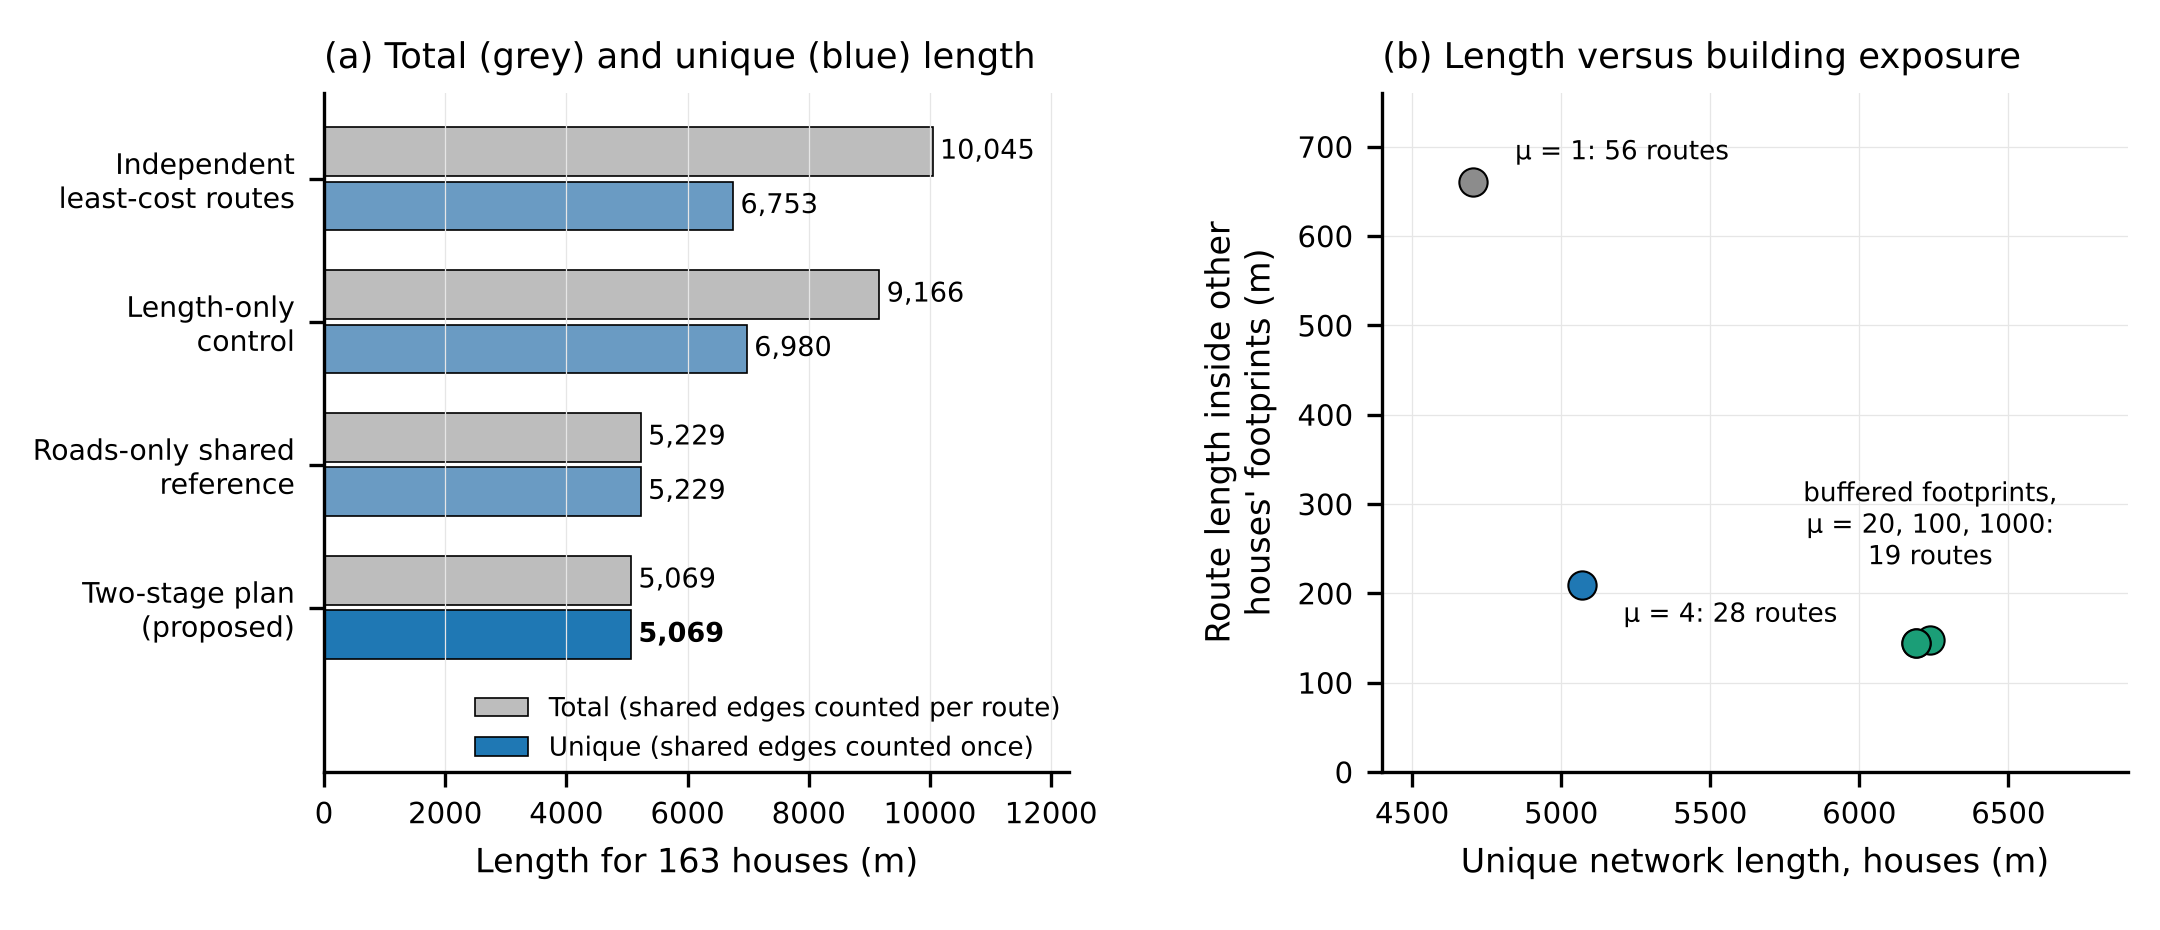
\includegraphics[width=\textwidth]{figures/fig3_routing.png}
\caption{Damarakunta routing results for 163 houses. (a)~Total and unique corridor length by strategy. (b)~Unique network length against route length inside other houses' footprints for $\mu=1$, $\mu=4$ and buffered footprints with large penalties.}
\label{fig:routing}
\end{figure}

\subsection{Impact of building omissions}
Table~\ref{tab:omission} and figure~\ref{fig:omission} summarise the omission analysis against the 5{,}069~m baseline. Missing buildings make the plan \emph{shorter}: 10\% random omission (16 houses) understates length by 7.6\%, 20\% by 16.9\%, omission of the smallest quarter by 25.1\% and omission of all merged blobs by 29.4\%. At the same time $U$ households lose access: 16 and 33 for random 10\% and 20\% omission, 41 for the smallest quarter and 62 (38.0\%) for merged blobs. A planner reading only total length would therefore underfund the scheme. Random additions lengthen the plan by 8.6\% and 15.8\%. The saving $\rho$ stays within 24.9--26.6\% across omissions, so the benefit of sharing is robust to inventory error.

\begin{table}[t]
\caption{Impact of simulated omissions and additions, Damarakunta. Baseline 5{,}069.0~m, 163 routed. Random scenarios are means of five draws. $U$: households without a route; $\kappa$: coverage; $\delta_L$: change in unique length; $\bar\ell$: length per routed target; $\rho$: saving against independent routing.}
\label{tab:omission}
\centering
\small
\begin{tabular}{@{}lrrrrrrr@{}}
\toprule
Scenario & Routed & $U$ & $\kappa$ (\%) & $L$ (m) & $\delta_L$ (\%) & $\bar\ell$ (m) & $\rho$ (\%)\\
\midrule
Baseline & 163 & 0 & 100.0 & 5{,}069.0 & 0.0 & 31.1 & 24.9\\
Omit 10\% (random) & 147.0 & 16 & 90.2 & 4{,}684.4 & $-7.6$ & 31.9 & 25.1\\
Omit 20\% (random) & 130.0 & 33 & 79.8 & 4{,}211.5 & $-16.9$ & 32.4 & 24.9\\
Omit smallest 10\% & 146 & 17 & 89.6 & 4{,}648.6 & $-8.3$ & 31.8 & 24.9\\
Omit smallest 25\% & 122 & 41 & 74.8 & 3{,}798.3 & $-25.1$ & 31.1 & 25.6\\
Omit merged blobs & 101 & 62 & 62.0 & 3{,}579.0 & $-29.4$ & 35.4 & 26.6\\
\midrule
Add 10\% (random) & 177.4 & --- & --- & 5{,}502.4 & $+8.6$ & 31.0 & 25.6\\
Add 20\% (random) & 190.6 & --- & --- & 5{,}868.3 & $+15.8$ & 30.8 & 25.4\\
\bottomrule
\end{tabular}
\end{table}

\begin{figure}[t]
\centering
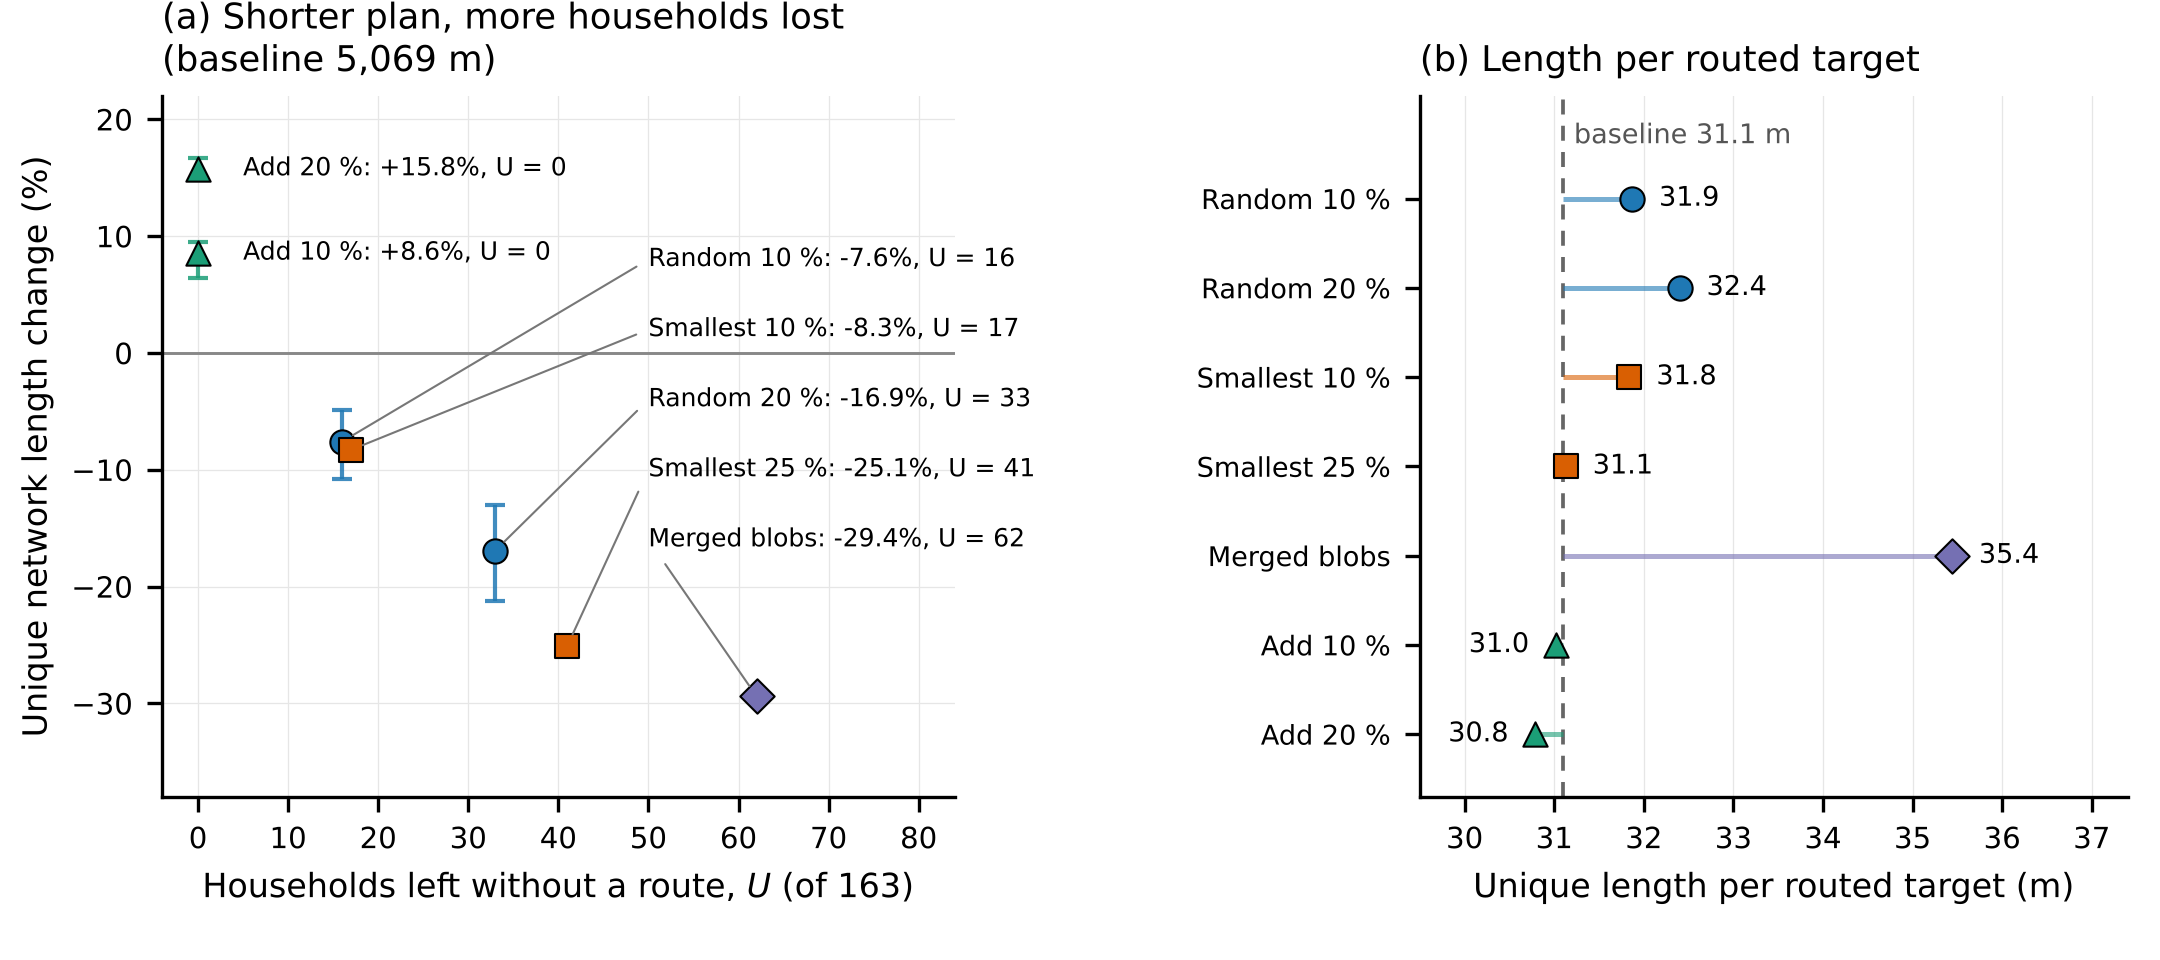
\includegraphics[width=\textwidth]{figures/fig4_omission.png}
\caption{Damarakunta omission sensitivity (163 baseline targets, 5{,}069~m; random scenarios are five draws with min--max bars). (a)~Change in unique length against households left without a route. (b)~Unique length per routed target.}
\label{fig:omission}
\end{figure}

\section{Results: transfer to Adilabad Urban}\label{sec:adilabad}
\subsection{Road-gap targets and routing}
\emph{End-to-end run (\dinoseg{} footprints).} Of the 2{,}690 footprints of at least 30~m$^2$, 345 lie more than 30~m from a road and form the targets (Damarakunta: 163). The planner routes all 345. Independent least-cost routes total 23{,}312.5~m (unique 21{,}440.8~m); the two-stage plan needs 18{,}288.7~m, a saving of 14.7\% (table~\ref{tab:adilabad}; the routes are drawn in figure~\ref{fig:flow}). The roads-only shared reference saves 2.3\% and the length-only control 6.9\%, so almost all of the saving comes from sharing among new routes. Exposure: 54 of 345 routes (15.7\%) cross another footprint (398.0~m), against 28 of 163 (17\%) in Damarakunta.

These numbers must be read with the extraction quality in mind. More than half of the instances (1{,}580 of 2{,}769) are \textsc{Unresolved\_Merge} blobs with a median area of 1{,}125.5~m$^2$: in the dense fabric the segmenter merges neighbouring roofs, so the 345 targets are built-up units rather than houses, and the footprint penalty acts on merged blocks. No reference mask exists for Adilabad, so detection accuracy there is not known.

\emph{Open-footprint check.} With 874 road-gap targets (873 routed) among 18{,}242 Overture footprints (median footprint 139.6~m$^2$, median distance to the nearest road 42.3~m), independent routes total 56{,}308.0~m (unique 46{,}419.2~m) and the two-stage plan 34{,}358.8~m, a saving of 26.0\%; the roads-only reference saves 2.9\% and the length-only control 5.7\%; 332 of 873 routes (38\%) cross another footprint (2{,}041.1~m). The facility phase connects 71 verified facilities with 1{,}090.1~m of unique corridor.

Both Adilabad variants agree that sharing helps (14.7\% and 26.0\%) and that a roads-only reference does not (2.3\% and 2.9\%, against 22.6\% in Damarakunta), but they differ in the size of the saving. This is consistent with fewer, more widely spaced targets (345 against 874) offering less opportunity to share, an explanation that was not tested. The comparison is between two footprint sources, not a validation of either.

\begin{table}[t]
\caption{Cross-settlement comparison under the same cost surface and solver. ``Seg.'' = \dinoseg{} footprints on Esri imagery; ``open'' = Overture footprints. Targets are defined by different rules (all candidates in Damarakunta, road-gap houses in Adilabad).}
\label{tab:adilabad}
\centering
\footnotesize
\begin{tabular}{@{}>{\raggedright\arraybackslash}p{5.6cm}rrr@{}}
\toprule
Metric & Damarakunta & Adilabad seg. & Adilabad open\\
\midrule
Study area (km$^2$) & 18.47 & 17.75 & 17.75\\
Targets / routed & 163 / 163 & 345 / 345 & 874 / 873\\
Independent routes, unique (m) & 6{,}753.1 & 21{,}440.8 & 46{,}419.2\\
Length-only control, unique (m) & 6{,}979.8 & 19{,}961.2 & 43{,}787.2\\
Roads-only shared reference, unique (m) & 5{,}229.3 & 20{,}947.0 & 45{,}058.9\\
\textbf{Two-stage plan, unique (m)} & \textbf{5{,}069.0} & \textbf{18{,}288.7} & \textbf{34{,}358.8}\\
Saving vs.\ independent (\%) & 24.9 & 14.7 & 26.0\\
Roads-only shared saving (\%) & 22.6 & 2.3 & 2.9\\
Unique length per routed house (m) & 31.1 & 53.0 & 39.4\\
Routes crossing other footprints & 28 of 163 & 54 of 345 & 332 of 873\\
Length inside other footprints (m) & 209.1 & 398.0 & 2{,}041.1\\
$\mu=1\rightarrow4$: unique length change (\%) & $+7.7$ & $+9.2$ & $+13.3$\\
$\mu=1\rightarrow4$: routes crossing & 56 $\rightarrow$ 28 & 138 $\rightarrow$ 54 & 618 $\rightarrow$ 332\\
10\% random omission: change (\%) / unserved & $-7.6$ / 16 & $-8.8$ / 34 & $-7.6$ / 88\\
20\% random omission: change (\%) / unserved & $-16.9$ / 33 & $-18.3$ / 69 & $-15.0$ / 176\\
Smallest-25\% omission: change (\%) / unserved & $-25.1$ / 41 & $-21.2$ / 87 & $-21.2$ / 220\\
\bottomrule
\end{tabular}
\end{table}
\subsection{Robustness}
\emph{Footprint penalty.} Raising $\mu$ from 1 to 4 lengthens the unique network by 9.2\% and removes 84 crossing routes (138 to 54); $\mu=20$ and 100 give 19{,}777.0~m and 19{,}924.5~m with 49 and 48 routes crossing, and buffered footprints give 22{,}757.0~m and 23{,}475.5~m with 7 crossing each (table~\ref{tab:sens}, figure~\ref{fig:adilsens}a). The saving against independent routing stays between 10.1\% and 17.7\% across all settings (open footprints: 17.8\% to 30.8\%, table~\ref{tab:sens_open}).

\emph{Road-gap threshold.} Targets defined as houses more than 20, 30 or 50~m from a road number 750, 345 and 129 and give savings of 10.6\%, 14.7\% and 18.5\% (open footprints: 2{,}190, 874 and 296 targets; 21.9\%, 26.0\% and 29.5\%). The saving therefore depends on the target definition, which should be reported with any such result.

\emph{Omissions.} Random omission of 10\% and 20\% (five seeds) changes unique length by $-8.8\%$ (range $-11.7$ to $-6.5$) and $-18.3\%$ ($-21.9$ to $-15.8$), leaving 34 and 69 targets unserved; single-run smallest-10\% and smallest-25\% omissions give $-8.0\%$ and $-21.2\%$ (35 and 87 unserved). As in Damarakunta and in the open-footprint check, missing buildings shorten the plan while stranding households, and the saving stays at 12.6--14.1\%. With open footprints the same scenarios give $-7.6\%$, $-15.0\%$, $-7.9\%$ and $-21.2\%$ and a saving of 23.8--25.2\%. Merged-blob and addition scenarios were not defined for Adilabad.

\begin{table}[t]
\caption{Adilabad sensitivity, \dinoseg{} footprints (345 targets unless stated). Top: footprint-penalty settings. Bottom: road-gap threshold.}
\label{tab:sens}
\centering
\footnotesize
\begin{tabular}{@{}lrrrrr@{}}
\toprule
Setting & Unique (m) & $\rho$ (\%) & Crossing routes & In footprints (m) & Targets\\
\midrule
Centre-in-footprint, $\mu=1$ & 16{,}740.5 & 17.7 & 138 & 1{,}479.8 & 345\\
Centre-in-footprint, $\mu=4$ & 18{,}288.7 & 14.7 & 54 & 398.0 & 345\\
Centre-in-footprint, $\mu=20$ & 19{,}777.0 & 12.5 & 49 & 356.4 & 345\\
Centre-in-footprint, $\mu=100$ & 19{,}924.5 & 12.2 & 48 & 343.2 & 345\\
Buffered 7.1~m, $\mu=20$ & 22{,}757.0 & 10.1 & 7 & 57.9 & 345\\
Buffered 7.1~m, $\mu=100$ & 23{,}475.5 & 10.6 & 7 & 55.7 & 345\\
\midrule
Gap $>20$~m & 30{,}621.7 & 10.6 & 69 & 442.8 & 750\\
Gap $>30$~m (primary) & 18{,}288.7 & 14.7 & 54 & 398.0 & 345\\
Gap $>50$~m & 9{,}155.2 & 18.5 & 28 & 251.9 & 129\\
\bottomrule
\end{tabular}
\end{table}

\begin{table}[t]
\caption{Adilabad sensitivity, open Overture footprints (874 targets, 873 routed). Top: footprint-penalty settings. Bottom: road-gap threshold.}
\label{tab:sens_open}
\centering
\footnotesize
\begin{tabular}{@{}lrrrrr@{}}
\toprule
Setting & Unique (m) & $\rho$ (\%) & Crossing routes & In footprints (m) & Targets\\
\midrule
Centre-in-footprint, $\mu=1$ & 30{,}335.7 & 30.8 & 618 & 4{,}893.0 & 874\\
Centre-in-footprint, $\mu=4$ & 34{,}358.8 & 26.0 & 332 & 2{,}041.1 & 874\\
Centre-in-footprint, $\mu=20$ & 37{,}024.1 & 22.8 & 271 & 1{,}687.4 & 874\\
Centre-in-footprint, $\mu=100$ & 37{,}513.9 & 21.7 & 275 & 1{,}744.8 & 874\\
Buffered 7.1~m, $\mu=20$ & 42{,}071.9 & 20.1 & 231 & 1{,}397.2 & 874\\
Buffered 7.1~m, $\mu=100$ & 44{,}094.6 & 17.8 & 221 & 1{,}310.5 & 874\\
\midrule
Gap $>20$~m & 65{,}204.4 & 21.9 & 815 & 4{,}543.9 & 2{,}190\\
Gap $>30$~m (primary) & 34{,}358.8 & 26.0 & 332 & 2{,}041.1 & 874\\
Gap $>50$~m & 15{,}880.9 & 29.5 & 126 & 809.9 & 296\\
\bottomrule
\end{tabular}
\end{table}

\begin{figure}[t]
\centering
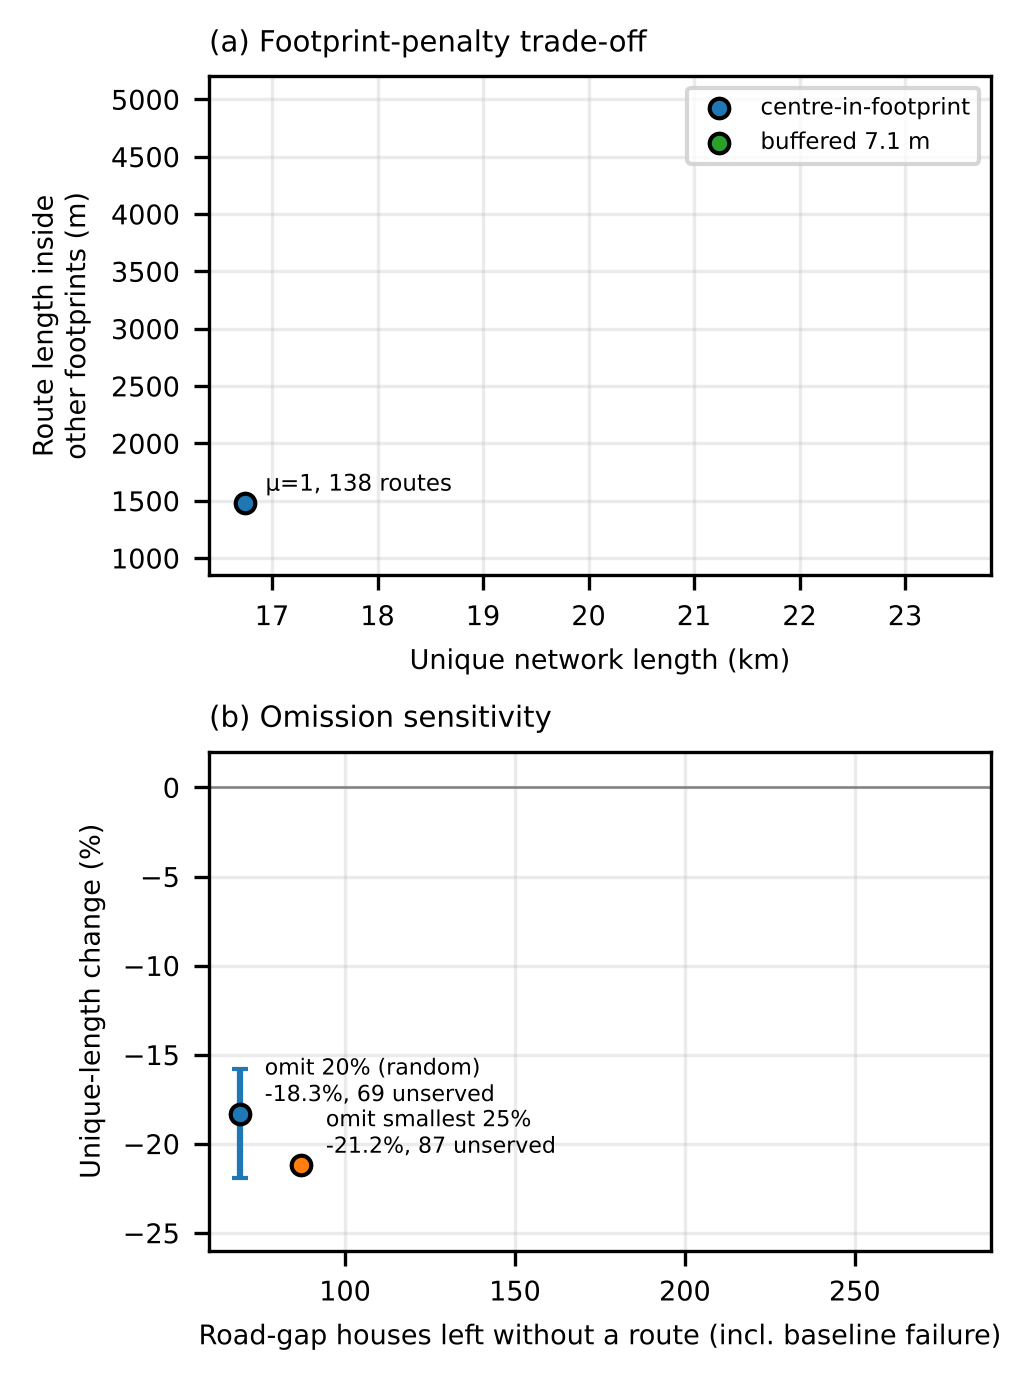
\includegraphics[width=0.5\textwidth]{figures/adilabad_seg_sens_col.png}
\caption{Adilabad sensitivity (\dinoseg{} footprints). (a)~Footprint-penalty trade-off between unique network length and route length inside other footprints. (b)~Omission sensitivity (random: mean and min--max over five seeds; smallest-$q$: single run).}
\label{fig:adilsens}
\end{figure}

\section{Results: four study areas with zero-crossing clearance}\label{sec:four}
Figure~\ref{fig:flow} follows the chain of figure~\ref{fig:arch} for the four study areas, from the Telangana locator through the input imagery and roads, the extracted footprints and verified facilities, to the planned network. Table~\ref{tab:four} collects every metric of the four areas in one place; it is regenerated by \texttt{scripts/run\_village\_pipeline.py --compare-all}, and a red \pending{value} marks a number not yet computed on the machine that wrote the table. The Adilabad column uses the updated settlement boundary (a derived built-up extent of Adilabad town) and the segmentation footprints of that boundary, so it is not the 2018 mandal experiment of the preceding sections.

On the 5~m clearance grid, Stage~B shortens the unique network relative to the independent Stage~A routes by Damarakunta 21.0\%, Adilabad 12.2\%, Aswaraopeta 25.3\%, Alampur 16.2\%. Building crossings are zero in every area by construction and were verified by intersecting every drawn route with all footprints, whereas the ten-metre soft-penalty plan ($\mu=4$) still leaves routes across other footprints (Damarakunta 28, Adilabad 99, Aswaraopeta 157, Alampur 5 routes, respectively). Targets with no free lane to the road network are reported as unrouted rather than routed over a roof, so the routed counts in table~\ref{tab:four} are below the target counts where buildings enclose a house. The segmentation rows are model-level: they are the LoveDA validation scores of the one checkpoint used for all four areas, not accuracy on any of the four areas, for which no surveyed reference exists. Costs use the owner-supplied, unverified PMGSY-based rate of Rs 75 lakh/km and are illustrative.

\begin{figure*}[p]
\centering
\IfFileExists{figures/fig_flow_study_areas.png}{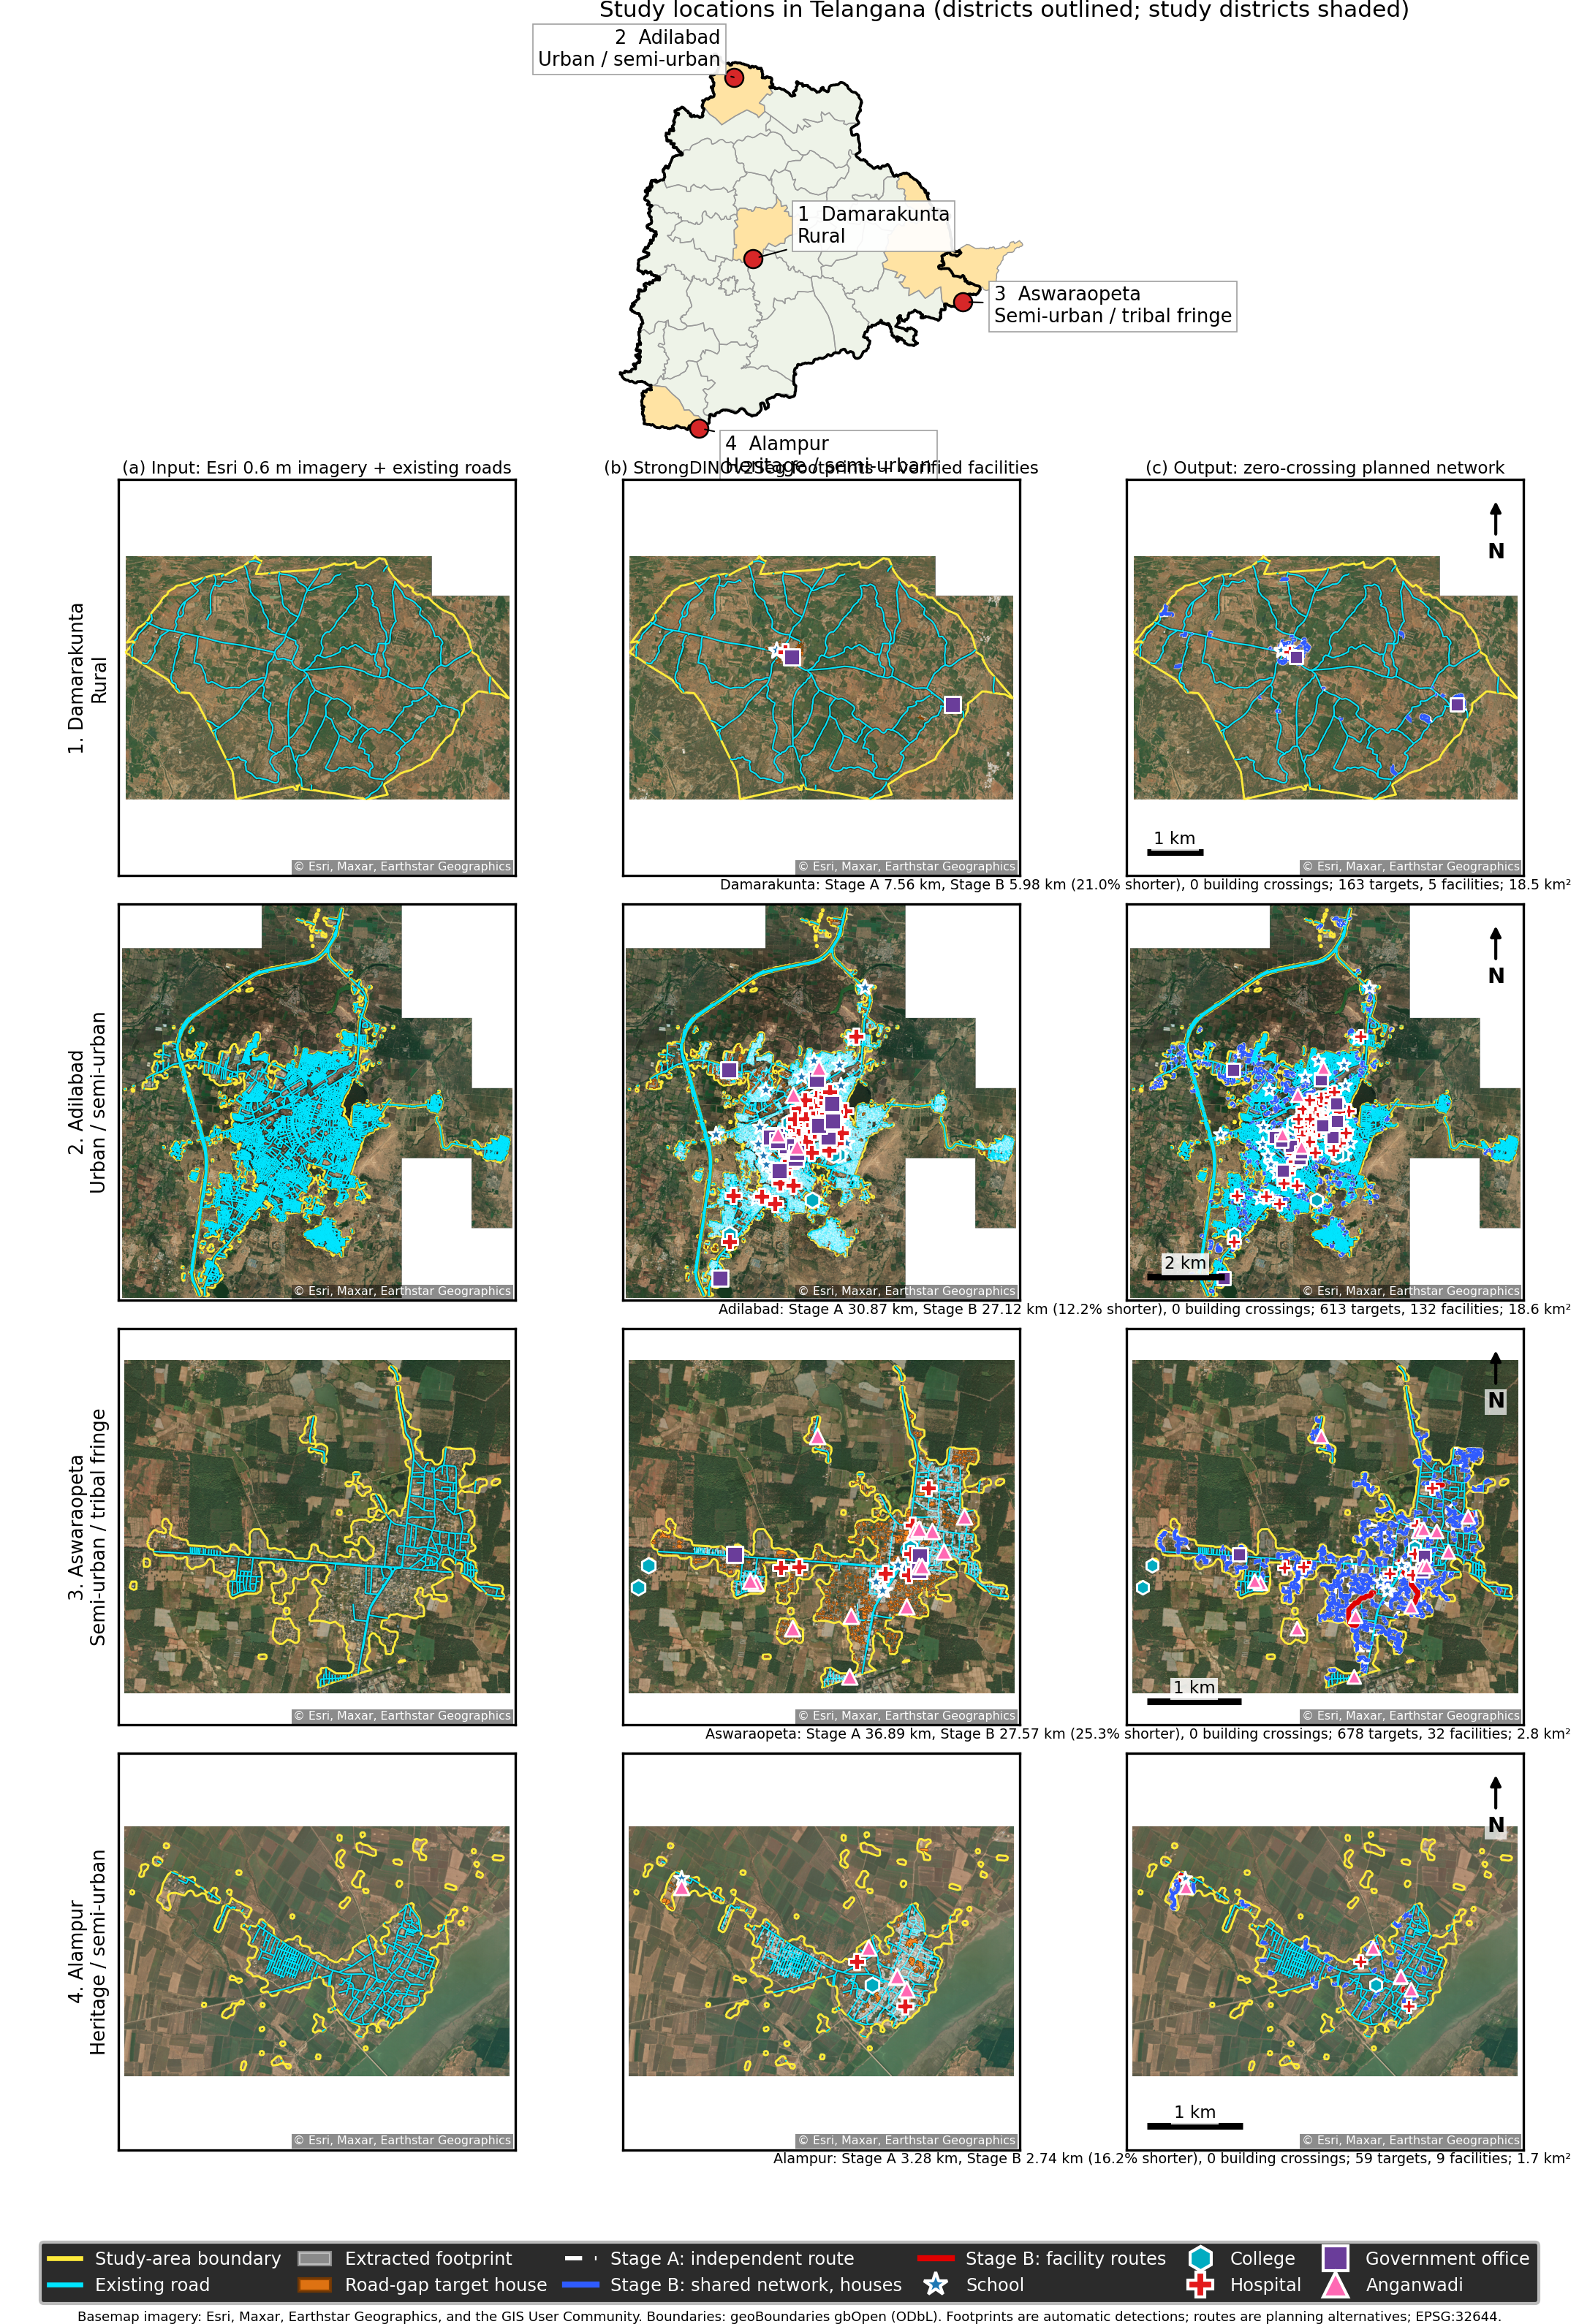
\includegraphics[width=0.93\textwidth]{figures/fig_flow_study_areas.png}}{\fbox{\parbox{0.8\textwidth}{\centering\pending{Figure not generated yet: run \texttt{python scripts/build\_paper\_flow\_figure.py --source segmentation} on the PC that holds the segmentation results.}}}}
\caption{Study areas and end-to-end flow. Top: Telangana with district outlines and the four study locations (1~Damarakunta, rural; 2~Adilabad, urban / semi-urban; 3~Aswaraopeta, semi-urban / tribal fringe; 4~Alampur, heritage / semi-urban). Rows 1--4: (a)~input, Esri World Imagery (0.6~m) with the existing road network; (b)~\dinoseg{} footprints (road-gap target houses in orange) with the verified facilities (School, College, Hospital, Government Office, Anganwadi); (c)~output, existing roads, Stage~A independent routes (white dashed) and Stage~B shared network (blue: houses; red: facilities) with the 5~m zero-crossing clearance, scale bar and north arrow. Basemap imagery: Esri, Maxar, Earthstar Geographics, and the GIS User Community. Footprints are automatic detections and routes are planning alternatives, not engineered roads.}
\label{fig:flow}
\end{figure*}

\begin{table*}[t]
\caption{Four study areas side by side. Segmentation rows: LoveDA validation of the single \dinoseg{} checkpoint (macro averages; F1-score equals the mean Dice). Routing rows: unique lengths on the 5~m zero-crossing grid (Stage~A independent, Stage~B shared network, shared edges once); building crossings are routes inside another building's footprint; the cost is the Stage~B length times Rs 75 lakh per km (range 60--90), an owner-supplied, unverified PMGSY-based rate, so it is illustrative and not an engineering estimate.}
\label{tab:four}
\centering
\scriptsize
\resizebox{\textwidth}{!}{% generated by scripts/run_village_pipeline.py --compare-all (do not edit by hand); \pending{...} marks a value not yet computed on the machine that generated this file
\begin{tabular}{@{}lrrrr@{}}
\toprule
Metric & Damarakunta & Adilabad & Aswaraopeta & Alampur \\
\midrule
\multicolumn{5}{@{}l}{\textit{Study area profile}}\\
District & Siddipet & Adilabad & Bhadradri Kothagudem & Jogulamba Gadwal \\
Typology & Rural & Urban / semi-urban & Semi-urban / tribal fringe & Heritage / semi-urban \\
Window area (km$^2$) & 18.47 & 18.59 & 2.82 & 1.65 \\
Existing road length (km) & 51.7 & 509.9 & 28.6 & 25.3 \\
\midrule
\multicolumn{5}{@{}l}{\textit{Segmentation and extraction (model metrics: LoveDA validation, one checkpoint for all areas)}}\\
Overall accuracy (\%) & \multicolumn{4}{c}{71.3} \\
Precision, macro (\%) & \multicolumn{4}{c}{72.4} \\
Recall, macro (\%) & \multicolumn{4}{c}{66.9} \\
F1-score = mean Dice (\%) & \multicolumn{4}{c}{68.9} \\
mIoU (\%) & \multicolumn{4}{c}{53.8} \\
Extracted building footprints & 165 & 5{,}653 & 1{,}297 & 430 \\
\midrule
\multicolumn{5}{@{}l}{\textit{Verified public infrastructure (audited, on building footprints)}}\\
School & 2 & 39 & 5 & 1 \\
College & 0 & 15 & 3 & 1 \\
Hospital & 1 & 59 & 7 & 2 \\
Government office & 2 & 15 & 3 & 0 \\
Anganwadi & 0 & 4 & 14 & 5 \\
Total verified facilities & 5 & 132 & 32 & 9 \\
\midrule
\multicolumn{5}{@{}l}{\textit{Stage A vs.\ Stage B routing (5\,m zero-crossing clearance) and PMGSY-benchmarked cost}}\\
Road-gap target buildings & 163 & 613 & 678 & 59 \\
Routed buildings & 162 & 607 & 632 & 58 \\
Stage A independent length (km) & 7.56 & 30.87 & 36.89 & 3.28 \\
Stage B shared-trunk length (km) & 5.98 & 27.12 & 27.57 & 2.74 \\
Corridor length saving (\%) & 21.0 & 12.2 & 25.3 & 16.2 \\
Building crossings (routes) & 0 & 0 & 0 & 0 \\
Mean terrain slope (\%) & 3.8 & 3.1 & 3.1 & 2.1 \\
PMGSY-benchmarked cost (INR lakh) & 448 & 2{,}034 & 2{,}067 & 206 \\
\bottomrule
\end{tabular}
% PMGSY-benchmarked cost = unique Stage B length (km) x Rs 75 lakh/km (sensitivity range 60-90)
}
\end{table*}

\section{Discussion}
\subsection{What transfers and what does not}
The planning stages transferred without modification: the same cost surface, solver parameters and metrics produced connected plans in a dense window, both from \dinoseg{} footprints on Esri imagery (345 targets) and from open footprints (874 targets). The qualitative findings were reproduced in all three settings: sharing saves unique length (24.9\%, 14.7\% and 26.0\%), the footprint penalty trades length for exposure, and omissions shorten the plan while stranding households. What did not transfer is the benefit of the simpler baselines: roads-only sharing recovered most of the gain in the dispersed village (22.6\%) but almost none in the dense window (2.3\% and 2.9\%), which suggests that the value of a marginal-cost planner grows with settlement density, a hypothesis supported by one dense window. The two Adilabad footprint sources differ in the size of the saving (14.7\% against 26.0\%); with 57\% of the segmented instances being merged blocks, the segmentation result may reflect coarse, widely spaced targets, and no reference mask exists to say which footprint set is closer to the truth.

\subsection{Why pixel metrics are not enough for infrastructure use}
Segmentation metrics are area-weighted over classes, while the planner counts instances. A detector that misses the smallest quarter of buildings can lose few building pixels yet removes a quarter of households from the plan (table~\ref{tab:omission}), and a detector that merges adjacent roofs can score a high pixel IoU yet strands 38\% of the Damarakunta houses in the merged-blob scenario. Network length falls in both cases, so total length is a poor quality indicator. Merged blobs correspond to dense multi-roof structures; whether they coincide with the core of a hamlet was not measured.

\subsection{Land take and planning use}
Shared corridors reduce the length of new road for the same households. As an illustration only, assuming a 5~m formation width (an assumption of this study; no road-width data were available), the 1{,}684~m saved in Damarakunta corresponds to about 0.84~ha less land take, the 3{,}152~m saved in Adilabad (segmentation targets) to about 1.6~ha and the 12{,}060~m saved against the open-footprint targets to about 6.0~ha. For PMGSY-style schemes \cite{pmgsy} three points follow. Building inventories are uncertain inputs and a network sized from them should carry a sensitivity band. Shared corridors save about a quarter of unique length and this survives omissions. Local overrides should be used sparingly and documented. The outputs are screening-level alternatives; we do not claim compliance with Indian Roads Congress design standards, nor any engineering design value.

\subsection{Limitations}
(i) Two settlements only; the semi-urban and second rural windows are planned but have not been run. (ii) Omission scenarios are synthetic, not measured detection errors. (iii) Neither Damarakunta nor Adilabad has a surveyed reference mask; the LoveDA metrics come from the epoch-4 checkpoint with metadata recovered from the training notebook, and the checkpoint hash (SHA-256 \texttt{2e7c4646dc77ceb2\allowbreak a357f44f11cb3f7f\allowbreak f84e636871d70ba4\allowbreak c31e194e5ec00cf3}) was logged only for the Adilabad run, not with the Damarakunta candidates, although both runs loaded the same file path. (iv) In Adilabad 57\% of the \dinoseg{} instances are \textsc{Unresolved\_Merge} blocks, so its 345 targets are built-up units, not houses; the open footprints are map data of unverified completeness, and Overture licences were not re-verified. Ten of the 68 verified facility points share an identical coordinate with another Overture record (generic geocodes), so the 20 m footprint check is weak evidence in the dense fabric. (v) Costs are ordinal, the planner is a heuristic without an optimality guarantee, and road-gap targeting changes the problem, as the threshold sweep shows. (vi) Pixel accuracy is reported as 71.3\%, the value recomputed from the confusion matrix. (vii) Merged-blob and addition scenarios were run only for Damarakunta.

\section{Conclusions}
A pipeline from satellite imagery and open layers to shared access roads connects the houses and facilities of a rural village (24.9\% less unique corridor than independent routing) and, without changes to the cost surface or solver, those of an urban and peri-urban mandal, end to end on Esri imagery (14.7\% less) and on open footprints (26.0\% less). Footprint penalties and simulated inventory errors behave consistently in all three settings: penalties trade length for fewer routes through dwellings, and omissions shorten the plan while stranding households. The dependence of the roads-only baseline on settlement density, and the effect of detection quality across settings, are the main open questions; a semi-urban and a second rural window are planned to address the first.

\ifanon\else
\section*{Acknowledgments}
The authors acknowledge the Telangana State Remote Sensing Application Centre (TGRAC) for the boundary, road and facility layers of Damarakunta, and the providers of the open datasets used (ESA WorldCover, Copernicus DEM, Overture Maps, geoBoundaries, Google Open Buildings, LoveDA).
\fi

\section*{Data sources and imagery attribution}
High-resolution RGB satellite basemap imagery for Damarakunta Village and the Adilabad Urban window was obtained via Esri World Imagery (sources: Esri, Maxar, Earthstar Geographics, and the GIS User Community) and used strictly for non-commercial academic research and visual overlay in accordance with Esri's academic use terms, while raw imagery tiles are not redistributed. All derived modeling and multi-settlement planning layers rely on open-licensed datasets: ESA WorldCover 10~m v200 (CC BY 4.0), Copernicus GLO-30 DEM (Copernicus Open Access Licence), geoBoundaries ADM3 (ODbL 1.0), and Overture Maps (ODbL 1.0 / CDLA-Permissive-2.0). Damarakunta's boundary, road and facility layers are TGRAC data and its $\sim$30~m DEM source was not recorded; the Copernicus GLO-30 and geoBoundaries layers apply to the Adilabad window.

\section*{Funding}
This research received no specific grant from any funding agency in the public, commercial, or not-for-profit sectors.

\section*{Data availability statement}
\ifanon
Code, derived tables and the open-data manifests (with SHA-256 hashes) will be made available in a public repository on acceptance and are available to reviewers on request. TGRAC layers for Damarakunta are subject to the provider's terms.
\else
Code, derived summary tables, and the open-data manifests with SHA-256 hashes are available at \url{https://github.com/Archana519/Telangana-Rural-Project} (folders \path{DELIVERABLES_DAMARAKUNTA_STAGE_B} and \path{DELIVERABLES_CONTRIBUTION_3_MULTI_VILLAGE}, the latter including the Adilabad segmentation results in \path{01_ADILABAD_SEGMENTATION}). TGRAC layers for Damarakunta are subject to the provider's terms. The \dinoseg{} checkpoint is not included in the repository; its SHA-256 is given in Section~\ref{sec:methods}. A Zenodo DOI will be added when the archive is minted.
\fi

\section*{Conflict of interest}
The authors declare no competing interests.

\bibliographystyle{unsrt}
\bibliography{references}

\end{document}
